%%
%% This is file `sample-sigconf-biblatex.tex',
%% generated with the docstrip utility.
%%
%% The original source files were:
%%
%% samples.dtx  (with options: `sigconf-biblatex')
%% 
%% IMPORTANT NOTICE:
%% 
%% For the copyright see the source file.
%% 
%% Any modified versions of this file must be renamed
%% with new filenames distinct from sample-sigconf-biblatex.tex.
%% 
%% For distribution of the original source see the terms
%% for copying and modification in the file samples.dtx.
%% 
%% This generated file may be distributed as long as the
%% original source files, as listed above, are part of the
%% same distribution. (The sources need not necessarily be
%% in the same archive or directory.)
%%
%%
%% Commands for TeXCount
%TC:macro \cite [option:text,text]
%TC:macro \citep [option:text,text]
%TC:macro \citet [option:text,text]
%TC:envir table 0 1
%TC:envir table* 0 1
%TC:envir tabular [ignore] word
%TC:envir displaymath 0 word
%TC:envir math 0 word
%TC:envir comment 0 0
%%
%%
%% The first command in your LaTeX source must be the \documentclass command.
\documentclass[sigconf, 10pt]{acmart}
% \documentclass[sigplan,10pt]{acmart}
\renewcommand\footnotetextcopyrightpermission[1]{}
\pagestyle{plain}

\settopmatter{printacmref=false, printccs=false, printfolios=true}
% Turn off footnotes under copyright
\renewcommand\footnotetextcopyrightpermission[1]{}

% Copyright
\setcopyright{none}% Turn off copyright

\acmConference[Conference'17]{}{xx}{xx}

%%
%% \BibTeX command to typeset BibTeX logo in the docs
% \AtBeginDocument{%
%   \providecommand\BibTeX{{%
%     Bib\TeX}}}

%% Rights management information.  This information is sent to you
%% when you complete the rights form.  These commands have SAMPLE
%% values in them; it is your responsibility as an author to replace
%% the commands and values with those provided to you when you
%% complete the rights form.
% \setcopyright{acmcopyright}
% \copyrightyear{2018}
% \acmYear{2018}
% \acmDOI{XXXXXXX.XXXXXXX}



%%
%% Submission ID.
%% Use this when submitting an article to a sponsored event. You'll
%% receive a unique submission ID from the organizers
%% of the event, and this ID should be used as the parameter to this command.
%%\acmSubmissionID{123-A56-BU3}

%%
%% For managing citations, it is recommended to use bibliography
%% files in BibTeX format.
%%
%% You can then either use BibTeX with the ACM-Reference-Format style,
%% or BibLaTeX with the acmnumeric or acmauthoryear sytles, that include
%% support for advanced citation of software artefact from the
%% biblatex-software package, also separately available on CTAN.
%%
%% Look at the sample-*-biblatex.tex files for templates showcasing
%% the biblatex styles.
%%


%%
%% The majority of ACM publications use numbered citations and
%% references, obtained by selecting the acmnumeric BibLaTeX style.
%% The acmauthoryear BibLaTeX style switches to the "author year" style.
%%
%% If you are preparing content for an event
%% sponsored by ACM SIGGRAPH, you must use the acmauthoryear style of
%% citations and references.
%%
% %% Bibliography style
% \RequirePackage[
%   datamodel=acmdatamodel,
%   style=acmnumeric,
%   ]{biblatex}

% %% Declare bibliography sources (one \addbibresource command per source)
% \addbibresource{references.bib}

% to be able to draw some self-contained figs
% \usepackage{tikz}
% \usepackage{amsmath}
% \usepackage{titling}

\usepackage{algorithm}
% \usepackage{amsthm}
% \usepackage{amssymb}
% \usepackage{multirow}
% \usepackage{tabls}
% \usepackage{bigstrut}
% \usepackage{comment}
\usepackage[noend]{algpseudocode}
% \usepackage{footmisc}
% \usepackage{ifthen}

%% Monospaced font
% \usepackage[T1]{fontenc}
% \usepackage{inconsolata}

% \usepackage{graphicx}
\usepackage{graphicx}
\usepackage{subfigure}
\usepackage{subcaption}
\usepackage{textcomp}
\usepackage{tabularx}
\usepackage{tabu}
\usepackage{longtable}
\usepackage{enumitem}
% \usepackage{cite}
\usepackage{makecell}
% \usepackage{flushend}
% \usepackage{listings}
% inlined bib file
% \usepackage{filecontents}
% \usepackage{xcolor}
\usepackage{multirow}
\usepackage{xspace}
\usepackage{url}
% \usepackage[binary-units]{siunitx}

\usepackage{booktabs}
\usepackage{graphicx}

\usepackage{balance}

% \pagenumbering{gobble}
\makeatletter
\def\do@url@hyp{\do\-\do\_}
\makeatother


\newcommand{\PHB}[1]{\noindent\textbf{#1}} % paragraph heading at the beginning of a section
\newcommand{\PHM}[1]{\noindent\textbf{#1}} % paragraph heading in the middle of a section


\newcommand{\SysName}{\texttt{$\lambda$Scale}\xspace}
\newcommand{\AlgoName}{\texttt{$\lambda$Pipe}\xspace}



\newcommand{\todo}[1]{\textcolor{blue}{TODO: #1}}
\newcommand{\revise}[1]{{#1}}


\newcommand{\circledNum}[1]{\raisebox{.5pt}{\textcircled{\raisebox{-.9pt} {#1}}}}


% rui
\usepackage[font=bf]{caption}

\graphicspath{{figures/}}


% \setlength{\droptitle}{-30pt}
% \posttitle{\par\end{center}}

%-------------------------------------------------------------------------------
\begin{document}
%-------------------------------------------------------------------------------


% make title bold and 14 pt font (Latex default is non-bold, 16 pt)
\title{\SysName: Enabling Fast Scaling for Serverless Large Language Model Inference}
% \title{Serverless Inference at Scale: Scaling to 100s of Large Model Instances from 0}

\author{
    \normalsize
    \textrm{Minchen Yu$^{\dag}$\textsuperscript{*}, Rui Yang$^{\ddag}$\textsuperscript{*}, Chaobo Jia$^{\dag}$, Zhaoyuan Su$^{\ddag}$, Sheng Yao$^{\S}$, Tingfeng Lan$^{\ddag}$, Yuchen Yang$^{\S}$, \\ Yue Cheng$^{\ddag}$,  Wei Wang$^{\S}$, Ao Wang$^{\diamond}$, and Ruichuan Chen$^{\triangle}$}\\
	$^{\dag}$The Chinese University of Hong Kong, Shenzhen \quad $^{\ddag}$University of Virginia  \\\quad $^{\S}$Hong Kong University of Science and Technology  \quad $^{\diamond}$Alibaba Group   \quad $^{\triangle}$Nokia Bell Labs 
}


\begin{abstract}  
Test time scaling is currently one of the most active research areas that shows promise after training time scaling has reached its limits.
Deep-thinking (DT) models are a class of recurrent models that can perform easy-to-hard generalization by assigning more compute to harder test samples.
However, due to their inability to determine the complexity of a test sample, DT models have to use a large amount of computation for both easy and hard test samples.
Excessive test time computation is wasteful and can cause the ``overthinking'' problem where more test time computation leads to worse results.
In this paper, we introduce a test time training method for determining the optimal amount of computation needed for each sample during test time.
We also propose Conv-LiGRU, a novel recurrent architecture for efficient and robust visual reasoning. 
Extensive experiments demonstrate that Conv-LiGRU is more stable than DT, effectively mitigates the ``overthinking'' phenomenon, and achieves superior accuracy.
\end{abstract}  
\maketitle
% \pagestyle{plain}
\renewcommand{\thefootnote}{*}
\footnotetext{Co-first authors.}
\renewcommand{\thefootnote}{\arabic{footnote}} 

\section{Introduction}
\label{sec:introduction}
The business processes of organizations are experiencing ever-increasing complexity due to the large amount of data, high number of users, and high-tech devices involved \cite{martin2021pmopportunitieschallenges, beerepoot2023biggestbpmproblems}. This complexity may cause business processes to deviate from normal control flow due to unforeseen and disruptive anomalies \cite{adams2023proceddsriftdetection}. These control-flow anomalies manifest as unknown, skipped, and wrongly-ordered activities in the traces of event logs monitored from the execution of business processes \cite{ko2023adsystematicreview}. For the sake of clarity, let us consider an illustrative example of such anomalies. Figure \ref{FP_ANOMALIES} shows a so-called event log footprint, which captures the control flow relations of four activities of a hypothetical event log. In particular, this footprint captures the control-flow relations between activities \texttt{a}, \texttt{b}, \texttt{c} and \texttt{d}. These are the causal ($\rightarrow$) relation, concurrent ($\parallel$) relation, and other ($\#$) relations such as exclusivity or non-local dependency \cite{aalst2022pmhandbook}. In addition, on the right are six traces, of which five exhibit skipped, wrongly-ordered and unknown control-flow anomalies. For example, $\langle$\texttt{a b d}$\rangle$ has a skipped activity, which is \texttt{c}. Because of this skipped activity, the control-flow relation \texttt{b}$\,\#\,$\texttt{d} is violated, since \texttt{d} directly follows \texttt{b} in the anomalous trace.
\begin{figure}[!t]
\centering
\includegraphics[width=0.9\columnwidth]{images/FP_ANOMALIES.png}
\caption{An example event log footprint with six traces, of which five exhibit control-flow anomalies.}
\label{FP_ANOMALIES}
\end{figure}

\subsection{Control-flow anomaly detection}
Control-flow anomaly detection techniques aim to characterize the normal control flow from event logs and verify whether these deviations occur in new event logs \cite{ko2023adsystematicreview}. To develop control-flow anomaly detection techniques, \revision{process mining} has seen widespread adoption owing to process discovery and \revision{conformance checking}. On the one hand, process discovery is a set of algorithms that encode control-flow relations as a set of model elements and constraints according to a given modeling formalism \cite{aalst2022pmhandbook}; hereafter, we refer to the Petri net, a widespread modeling formalism. On the other hand, \revision{conformance checking} is an explainable set of algorithms that allows linking any deviations with the reference Petri net and providing the fitness measure, namely a measure of how much the Petri net fits the new event log \cite{aalst2022pmhandbook}. Many control-flow anomaly detection techniques based on \revision{conformance checking} (hereafter, \revision{conformance checking}-based techniques) use the fitness measure to determine whether an event log is anomalous \cite{bezerra2009pmad, bezerra2013adlogspais, myers2018icsadpm, pecchia2020applicationfailuresanalysispm}. 

The scientific literature also includes many \revision{conformance checking}-independent techniques for control-flow anomaly detection that combine specific types of trace encodings with machine/deep learning \cite{ko2023adsystematicreview, tavares2023pmtraceencoding}. Whereas these techniques are very effective, their explainability is challenging due to both the type of trace encoding employed and the machine/deep learning model used \cite{rawal2022trustworthyaiadvances,li2023explainablead}. Hence, in the following, we focus on the shortcomings of \revision{conformance checking}-based techniques to investigate whether it is possible to support the development of competitive control-flow anomaly detection techniques while maintaining the explainable nature of \revision{conformance checking}.
\begin{figure}[!t]
\centering
\includegraphics[width=\columnwidth]{images/HIGH_LEVEL_VIEW.png}
\caption{A high-level view of the proposed framework for combining \revision{process mining}-based feature extraction with dimensionality reduction for control-flow anomaly detection.}
\label{HIGH_LEVEL_VIEW}
\end{figure}

\subsection{Shortcomings of \revision{conformance checking}-based techniques}
Unfortunately, the detection effectiveness of \revision{conformance checking}-based techniques is affected by noisy data and low-quality Petri nets, which may be due to human errors in the modeling process or representational bias of process discovery algorithms \cite{bezerra2013adlogspais, pecchia2020applicationfailuresanalysispm, aalst2016pm}. Specifically, on the one hand, noisy data may introduce infrequent and deceptive control-flow relations that may result in inconsistent fitness measures, whereas, on the other hand, checking event logs against a low-quality Petri net could lead to an unreliable distribution of fitness measures. Nonetheless, such Petri nets can still be used as references to obtain insightful information for \revision{process mining}-based feature extraction, supporting the development of competitive and explainable \revision{conformance checking}-based techniques for control-flow anomaly detection despite the problems above. For example, a few works outline that token-based \revision{conformance checking} can be used for \revision{process mining}-based feature extraction to build tabular data and develop effective \revision{conformance checking}-based techniques for control-flow anomaly detection \cite{singh2022lapmsh, debenedictis2023dtadiiot}. However, to the best of our knowledge, the scientific literature lacks a structured proposal for \revision{process mining}-based feature extraction using the state-of-the-art \revision{conformance checking} variant, namely alignment-based \revision{conformance checking}.

\subsection{Contributions}
We propose a novel \revision{process mining}-based feature extraction approach with alignment-based \revision{conformance checking}. This variant aligns the deviating control flow with a reference Petri net; the resulting alignment can be inspected to extract additional statistics such as the number of times a given activity caused mismatches \cite{aalst2022pmhandbook}. We integrate this approach into a flexible and explainable framework for developing techniques for control-flow anomaly detection. The framework combines \revision{process mining}-based feature extraction and dimensionality reduction to handle high-dimensional feature sets, achieve detection effectiveness, and support explainability. Notably, in addition to our proposed \revision{process mining}-based feature extraction approach, the framework allows employing other approaches, enabling a fair comparison of multiple \revision{conformance checking}-based and \revision{conformance checking}-independent techniques for control-flow anomaly detection. Figure \ref{HIGH_LEVEL_VIEW} shows a high-level view of the framework. Business processes are monitored, and event logs obtained from the database of information systems. Subsequently, \revision{process mining}-based feature extraction is applied to these event logs and tabular data input to dimensionality reduction to identify control-flow anomalies. We apply several \revision{conformance checking}-based and \revision{conformance checking}-independent framework techniques to publicly available datasets, simulated data of a case study from railways, and real-world data of a case study from healthcare. We show that the framework techniques implementing our approach outperform the baseline \revision{conformance checking}-based techniques while maintaining the explainable nature of \revision{conformance checking}.

In summary, the contributions of this paper are as follows.
\begin{itemize}
    \item{
        A novel \revision{process mining}-based feature extraction approach to support the development of competitive and explainable \revision{conformance checking}-based techniques for control-flow anomaly detection.
    }
    \item{
        A flexible and explainable framework for developing techniques for control-flow anomaly detection using \revision{process mining}-based feature extraction and dimensionality reduction.
    }
    \item{
        Application to synthetic and real-world datasets of several \revision{conformance checking}-based and \revision{conformance checking}-independent framework techniques, evaluating their detection effectiveness and explainability.
    }
\end{itemize}

The rest of the paper is organized as follows.
\begin{itemize}
    \item Section \ref{sec:related_work} reviews the existing techniques for control-flow anomaly detection, categorizing them into \revision{conformance checking}-based and \revision{conformance checking}-independent techniques.
    \item Section \ref{sec:abccfe} provides the preliminaries of \revision{process mining} to establish the notation used throughout the paper, and delves into the details of the proposed \revision{process mining}-based feature extraction approach with alignment-based \revision{conformance checking}.
    \item Section \ref{sec:framework} describes the framework for developing \revision{conformance checking}-based and \revision{conformance checking}-independent techniques for control-flow anomaly detection that combine \revision{process mining}-based feature extraction and dimensionality reduction.
    \item Section \ref{sec:evaluation} presents the experiments conducted with multiple framework and baseline techniques using data from publicly available datasets and case studies.
    \item Section \ref{sec:conclusions} draws the conclusions and presents future work.
\end{itemize}
\section{Background}\label{sec:backgrnd}

\subsection{Cold Start Latency and Mitigation Techniques}

Traditional FaaS platforms mitigate cold starts through snapshotting, lightweight virtualization, and warm-state management. Snapshot-based methods like \textbf{REAP} and \textbf{Catalyzer} reduce initialization time by preloading or restoring container states but require significant memory and I/O resources, limiting scalability~\cite{dong_catalyzer_2020, ustiugov_benchmarking_2021}. Lightweight virtualization solutions, such as \textbf{Firecracker} microVMs, achieve fast startup times with strong isolation but depend on robust infrastructure, making them less adaptable to fluctuating workloads~\cite{agache_firecracker_2020}. Warm-state management techniques like \textbf{Faa\$T}~\cite{romero_faa_2021} and \textbf{Kraken}~\cite{vivek_kraken_2021} keep frequently invoked containers ready, balancing readiness and cost efficiency under predictable workloads but incurring overhead when demand is erratic~\cite{romero_faa_2021, vivek_kraken_2021}. While these methods perform well in resource-rich cloud environments, their resource intensity challenges applicability in edge settings.

\subsubsection{Edge FaaS Perspective}

In edge environments, cold start mitigation emphasizes lightweight designs, resource sharing, and hybrid task distribution. Lightweight execution environments like unikernels~\cite{edward_sock_2018} and \textbf{Firecracker}~\cite{agache_firecracker_2020}, as used by \textbf{TinyFaaS}~\cite{pfandzelter_tinyfaas_2020}, minimize resource usage and initialization delays but require careful orchestration to avoid resource contention. Function co-location, demonstrated by \textbf{Photons}~\cite{v_dukic_photons_2020}, reduces redundant initializations by sharing runtime resources among related functions, though this complicates isolation in multi-tenant setups~\cite{v_dukic_photons_2020}. Hybrid offloading frameworks like \textbf{GeoFaaS}~\cite{malekabbasi_geofaas_2024} balance edge-cloud workloads by offloading latency-tolerant tasks to the cloud and reserving edge resources for real-time operations, requiring reliable connectivity and efficient task management. These edge-specific strategies address cold starts effectively but introduce challenges in scalability and orchestration.

\subsection{Predictive Scaling and Caching Techniques}

Efficient resource allocation is vital for maintaining low latency and high availability in serverless platforms. Predictive scaling and caching techniques dynamically provision resources and reduce cold start latency by leveraging workload prediction and state retention.
Traditional FaaS platforms use predictive scaling and caching to optimize resources, employing techniques (OFC, FaasCache) to reduce cold starts. However, these methods rely on centralized orchestration and workload predictability, limiting their effectiveness in dynamic, resource-constrained edge environments.



\subsubsection{Edge FaaS Perspective}

Edge FaaS platforms adapt predictive scaling and caching techniques to constrain resources and heterogeneous environments. \textbf{EDGE-Cache}~\cite{kim_delay-aware_2022} uses traffic profiling to selectively retain high-priority functions, reducing memory overhead while maintaining readiness for frequent requests. Hybrid frameworks like \textbf{GeoFaaS}~\cite{malekabbasi_geofaas_2024} implement distributed caching to balance resources between edge and cloud nodes, enabling low-latency processing for critical tasks while offloading less critical workloads. Machine learning methods, such as clustering-based workload predictors~\cite{gao_machine_2020} and GRU-based models~\cite{guo_applying_2018}, enhance resource provisioning in edge systems by efficiently forecasting workload spikes. These innovations effectively address cold start challenges in edge environments, though their dependency on accurate predictions and robust orchestration poses scalability challenges.

\subsection{Decentralized Orchestration, Function Placement, and Scheduling}

Efficient orchestration in serverless platforms involves workload distribution, resource optimization, and performance assurance. While traditional FaaS platforms rely on centralized control, edge environments require decentralized and adaptive strategies to address unique challenges such as resource constraints and heterogeneous hardware.



\subsubsection{Edge FaaS Perspective}

Edge FaaS platforms adopt decentralized and adaptive orchestration frameworks to meet the demands of resource-constrained environments. Systems like \textbf{Wukong} distribute scheduling across edge nodes, enhancing data locality and scalability while reducing network latency. Lightweight frameworks such as \textbf{OpenWhisk Lite}~\cite{kravchenko_kpavelopenwhisk-light_2024} optimize resource allocation by decentralizing scheduling policies, minimizing cold starts and latency in edge setups~\cite{benjamin_wukong_2020}. Hybrid solutions like \textbf{OpenFaaS}~\cite{noauthor_openfaasfaas_2024} and \textbf{EdgeMatrix}~\cite{shen_edgematrix_2023} combine edge-cloud orchestration to balance resource utilization, retaining latency-sensitive functions at the edge while offloading non-critical workloads to the cloud. While these approaches improve flexibility, they face challenges in maintaining coordination and ensuring consistent performance across distributed nodes.


\section{Overview}

\revision{In this section, we first explain the foundational concept of Hausdorff distance-based penetration depth algorithms, which are essential for understanding our method (Sec.~\ref{sec:preliminary}).
We then provide a brief overview of our proposed RT-based penetration depth algorithm (Sec.~\ref{subsec:algo_overview}).}



\section{Preliminaries }
\label{sec:Preliminaries}

% Before we introduce our method, we first overview the important basics of 3D dynamic human modeling with Gaussian splatting. Then, we discuss the diffusion-based 3d generation techniques, and how they can be applied to human modeling.
% \ZY{I stopp here. TBC.}
% \subsection{Dynamic human modeling with Gaussian splatting}
\subsection{3D Gaussian Splatting}
3D Gaussian splatting~\cite{kerbl3Dgaussians} is an explicit scene representation that allows high-quality real-time rendering. The given scene is represented by a set of static 3D Gaussians, which are parameterized as follows: Gaussian center $x\in {\mathbb{R}^3}$, color $c\in {\mathbb{R}^3}$, opacity $\alpha\in {\mathbb{R}}$, spatial rotation in the form of quaternion $q\in {\mathbb{R}^4}$, and scaling factor $s\in {\mathbb{R}^3}$. Given these properties, the rendering process is represented as:
\begin{equation}
  I = Splatting(x, c, s, \alpha, q, r),
  \label{eq:splattingGA}
\end{equation}
where $I$ is the rendered image, $r$ is a set of query rays crossing the scene, and $Splatting(\cdot)$ is a differentiable rendering process. We refer readers to Kerbl et al.'s paper~\cite{kerbl3Dgaussians} for the details of Gaussian splatting. 



% \ZY{I would suggest move this part to the method part.}
% GaissianAvatar is a dynamic human generation model based on Gaussian splitting. Given a sequence of RGB images, this method utilizes fitted SMPLs and sampled points on its surface to obtain a pose-dependent feature map by a pose encoder. The pose-dependent features and a geometry feature are fed in a Gaussian decoder, which is employed to establish a functional mapping from the underlying geometry of the human form to diverse attributes of 3D Gaussians on the canonical surfaces. The parameter prediction process is articulated as follows:
% \begin{equation}
%   (\Delta x,c,s)=G_{\theta}(S+P),
%   \label{eq:gaussiandecoder}
% \end{equation}
%  where $G_{\theta}$ represents the Gaussian decoder, and $(S+P)$ is the multiplication of geometry feature S and pose feature P. Instead of optimizing all attributes of Gaussian, this decoder predicts 3D positional offset $\Delta{x} \in {\mathbb{R}^3}$, color $c\in\mathbb{R}^3$, and 3D scaling factor $ s\in\mathbb{R}^3$. To enhance geometry reconstruction accuracy, the opacity $\alpha$ and 3D rotation $q$ are set to fixed values of $1$ and $(1,0,0,0)$ respectively.
 
%  To render the canonical avatar in observation space, we seamlessly combine the Linear Blend Skinning function with the Gaussian Splatting~\cite{kerbl3Dgaussians} rendering process: 
% \begin{equation}
%   I_{\theta}=Splatting(x_o,Q,d),
%   \label{eq:splatting}
% \end{equation}
% \begin{equation}
%   x_o = T_{lbs}(x_c,p,w),
%   \label{eq:LBS}
% \end{equation}
% where $I_{\theta}$ represents the final rendered image, and the canonical Gaussian position $x_c$ is the sum of the initial position $x$ and the predicted offset $\Delta x$. The LBS function $T_{lbs}$ applies the SMPL skeleton pose $p$ and blending weights $w$ to deform $x_c$ into observation space as $x_o$. $Q$ denotes the remaining attributes of the Gaussians. With the rendering process, they can now reposition these canonical 3D Gaussians into the observation space.



\subsection{Score Distillation Sampling}
Score Distillation Sampling (SDS)~\cite{poole2022dreamfusion} builds a bridge between diffusion models and 3D representations. In SDS, the noised input is denoised in one time-step, and the difference between added noise and predicted noise is considered SDS loss, expressed as:

% \begin{equation}
%   \mathcal{L}_{SDS}(I_{\Phi}) \triangleq E_{t,\epsilon}[w(t)(\epsilon_{\phi}(z_t,y,t)-\epsilon)\frac{\partial I_{\Phi}}{\partial\Phi}],
%   \label{eq:SDSObserv}
% \end{equation}
\begin{equation}
    \mathcal{L}_{\text{SDS}}(I_{\Phi}) \triangleq \mathbb{E}_{t,\epsilon} \left[ w(t) \left( \epsilon_{\phi}(z_t, y, t) - \epsilon \right) \frac{\partial I_{\Phi}}{\partial \Phi} \right],
  \label{eq:SDSObservGA}
\end{equation}
where the input $I_{\Phi}$ represents a rendered image from a 3D representation, such as 3D Gaussians, with optimizable parameters $\Phi$. $\epsilon_{\phi}$ corresponds to the predicted noise of diffusion networks, which is produced by incorporating the noise image $z_t$ as input and conditioning it with a text or image $y$ at timestep $t$. The noise image $z_t$ is derived by introducing noise $\epsilon$ into $I_{\Phi}$ at timestep $t$. The loss is weighted by the diffusion scheduler $w(t)$. 
% \vspace{-3mm}

\subsection{Overview of the RTPD Algorithm}\label{subsec:algo_overview}
Fig.~\ref{fig:Overview} presents an overview of our RTPD algorithm.
It is grounded in the Hausdorff distance-based penetration depth calculation method (Sec.~\ref{sec:preliminary}).
%, similar to that of Tang et al.~\shortcite{SIG09HIST}.
The process consists of two primary phases: penetration surface extraction and Hausdorff distance calculation.
We leverage the RTX platform's capabilities to accelerate both of these steps.

\begin{figure*}[t]
    \centering
    \includegraphics[width=0.8\textwidth]{Image/overview.pdf}
    \caption{The overview of RT-based penetration depth calculation algorithm overview}
    \label{fig:Overview}
\end{figure*}

The penetration surface extraction phase focuses on identifying the overlapped region between two objects.
\revision{The penetration surface is defined as a set of polygons from one object, where at least one of its vertices lies within the other object. 
Note that in our work, we focus on triangles rather than general polygons, as they are processed most efficiently on the RTX platform.}
To facilitate this extraction, we introduce a ray-tracing-based \revision{Point-in-Polyhedron} test (RT-PIP), significantly accelerated through the use of RT cores (Sec.~\ref{sec:RT-PIP}).
This test capitalizes on the ray-surface intersection capabilities of the RTX platform.
%
Initially, a Geometry Acceleration Structure (GAS) is generated for each object, as required by the RTX platform.
The RT-PIP module takes the GAS of one object (e.g., $GAS_{A}$) and the point set of the other object (e.g., $P_{B}$).
It outputs a set of points (e.g., $P_{\partial B}$) representing the penetration region, indicating their location inside the opposing object.
Subsequently, a penetration surface (e.g., $\partial B$) is constructed using this point set (e.g., $P_{\partial B}$) (Sec.~\ref{subsec:surfaceGen}).
%
The generated penetration surfaces (e.g., $\partial A$ and $\partial B$) are then forwarded to the next step. 

The Hausdorff distance calculation phase utilizes the ray-surface intersection test of the RTX platform (Sec.~\ref{sec:RT-Hausdorff}) to compute the Hausdorff distance between two objects.
We introduce a novel Ray-Tracing-based Hausdorff DISTance algorithm, RT-HDIST.
It begins by generating GAS for the two penetration surfaces, $P_{\partial A}$ and $P_{\partial B}$, derived from the preceding step.
RT-HDIST processes the GAS of a penetration surface (e.g., $GAS_{\partial A}$) alongside the point set of the other penetration surface (e.g., $P_{\partial B}$) to compute the penetration depth between them.
The algorithm operates bidirectionally, considering both directions ($\partial A \to \partial B$ and $\partial B \to \partial A$).
The final penetration depth between the two objects, A and B, is determined by selecting the larger value from these two directional computations.

%In the Hausdorff distance calculation step, we compute the Hausdorff distance between given two objects using a ray-surface-intersection test. (Sec.~\ref{sec:RT-Hausdorff}) Initially, we construct the GAS for both $\partial A$ and $\partial B$ to utilize the RT-core effectively. The RT-based Hausdorff distance algorithms then determine the Hausdorff distance by processing the GAS of one object (e.g. $GAS_{\partial A}$) and set of the vertices of the other (e.g. $P_{\partial B}$). Following the Hausdorff distance definition (Eq.~\ref{equation:hausdorff_definition}), we compute the Hausdorff distance to both directions ($\partial A \to \partial B$) and ($\partial B \to \partial A$). As a result, the bigger one is the final Hausdorff distance, and also it is the penetration depth between input object $A$ and $B$.


%the proposed RT-based penetration depth calculation pipeline.
%Our proposed methods adopt Tang's Hausdorff-based penetration depth methods~\cite{SIG09HIST}. The pipeline is divided into the penetration surface extraction step and the Hausdorff distance calculation between the penetration surface steps. However, since Tang's approach is not suitable for the RT platform in detail, we modified and applied it with appropriate methods.

%The penetration surface extraction step is extracting overlapped surfaces on other objects. To utilize the RT core, we use the ray-intersection-based PIP(Point-In-Polygon) algorithms instead of collision detection between two objects which Tang et al.~\cite{SIG09HIST} used. (Sec.~\ref{sec:RT-PIP})
%RT core-based PIP test uses a ray-surface intersection test. For purpose this, we generate the GAS(Geometry Acceleration Structure) for each object. RT core-based PIP test takes the GAS of one object (e.g. $GAS_{A}$) and a set of vertex of another one (e.g. $P_{B}$). Then this computes the penetrated vertex set of another one (e.g. $P_{\partial B}$). To calculate the Hausdorff distance, these vertex sets change to objects constructed by penetrated surface (e.g. $\partial B$). Finally, the two generated overlapped surface objects $\partial A$ and $\partial B$ are used in the Hausdorff distance calculation step.
\begin{algorithm}[ht!]
\caption{\textit{NovelSelect}}
\label{alg:novelselect}
\begin{algorithmic}[1]
\State \textbf{Input:} Data pool $\mathcal{X}^{all}$, data budget $n$
\State Initialize an empty dataset, $\mathcal{X} \gets \emptyset$
\While{$|\mathcal{X}| < n$}
    \State $x^{new} \gets \arg\max_{x \in \mathcal{X}^{all}} v(x)$
    \State $\mathcal{X} \gets \mathcal{X} \cup \{x^{new}\}$
    \State $\mathcal{X}^{all} \gets \mathcal{X}^{all} \setminus \{x^{new}\}$
\EndWhile
\State \textbf{return} $\mathcal{X}$
\end{algorithmic}
\end{algorithm}


%PlanGREEN

%GEN-Plan

%G- generate
%R-refine
%E- edit

%% GREEN-plan

%% PURPLE
\begin{figure*}
    \centering
    \Description{PLAID's system architecture diagram. Top part shows the database (a), and bottom part shows the interface (b). The system starts from bottom right as an instructor is interested in a programming domain, then the pipeline described in the text produces reference materials at different levels of granularity, and these are presented in the interface.}
    \includegraphics[width=\textwidth]{img/system-architecture-subgoals.png}
    \caption{PLAID's reference content is generated through an LLM pipeline
    %inspired by the practices of instructors who have successfully identified programming plans. 
    that produces output on three levels.
    First, a wide variety of use cases are generated to create example programs that focus on code's applications. Next, using LLM's explanatory comments that represent subgoals within the code, the examples are segmented into meaningful code snippets. The LLM is queried to generate other plan components for each code snippet. Finally, the code snippets are clustered to identify the most common patterns, representing plan candidates. The full programs are presented in `Programs' views of PLAID interface, whereas snippets are presented in clusters in the `Plan Creation' view.}
    \label{fig:system-pipeline}
\end{figure*}
\section{PLAID: A System for Supporting Plan Identification}
\label{sec:system-design}

Following the design goals devised from the design workshop, we refined our early prototype into PLAID: a
%LLM-powered
tool to assist instructors in their plan identification process.
PLAID synthesizes the capabilities of LLMs in code generation with interactions enabling plan identification practices observed in our studies with instructors.
As we noted in the findings of our design workshop, the LLM-generated candidate plans are not ready to be used as is in instruction, but instructors can readily adapt and correct them (\cref{sec:workshop-findings-condition2}).
PLAID enables collaboration between instructors and LLMs, enhancing the plan identification process by automating its time-intensive information-gathering tasks and facilitating instructors' ability to refine LLM-generated candidate plans based on their knowledge about pedagogy and the programming domain. 



\subsection{Practical Illustration}

To understand how instructors use can PLAID to more easily adopt plan-based pedagogies, we follow Jane, a computer science instructor using PLAID to design programming plans for her course (summarized in \cref{fig:jane-workflow}).

Jane is teaching a programming course for psychology majors and wants to introduce her students to data analysis using Pandas. As her students have limited prior programming experience and use programming for specific goals, she organizes her lecture material around programming plans to emphasize purpose over syntax. 
% that explain practical concepts to students and help them focus on the purpose behind the code they write.
% However, she realizes that all introductory computer science courses offered at her institution only teach basic programming constructs like data structures. After exploring Google Scholar for effective instructional methods to teach application-focused programming to non-computer science majors, she learned about plan-based pedagogies that help them focus on the purpose behind the code they write. In her literature review, she finds out about PLAID, a tool that can help her design domain-specific plans. She reviews the domains supported by the tool (Pandas, Pytorch, Beautifulsoup, and Django) and decides to use Pandas, a popular and powerful data analysis and manipulation library, to create her curriculum. 

She logs in to the PLAID web interface, % and takes time to explore the system's features. 
and asks PLAID to suggest a plan (\cref{fig:jane-workflow}, 1). The first plan recommended to her 
% she sees is a plan to help students learn about
is about reading CSV files. 
She thinks the topic is important and the solution code aligns with her experience; % the solution is promising and represents an important concept that students need to know about.
% She is satisfied with the given solution 
but she finds the generated name and goal to be too generic. She edits (\cref{fig:jane-workflow}, 2) these fields to provide more context that she feels is right for her students.
% She refines those fields and then 
To make this plan more abstract and appropriate for more use cases, %explain how this plan can be used for reading data from different file formats,
she marks the file path as a changeable area (\cref{fig:jane-workflow}, 3), generalizing the plan for reading data from different file formats.

Inspired by the first plan, she decides to create a plan for saving data to disk. She wants to teach the most conventional way of saving data, so she switches to the use case tab (\cref{fig:jane-workflow}, 4) and explores example programs that save data to get a sense of common practices.  %interact with the list of complete programs.
She finds a complete example where a DataFrame is created and and saved to a file. %performs cleaning tasks like deleting NaN values, and exports it.
% She realizes that something she hadn't thought of before: saving new data is almost always necessary after performing data manipulation operations!
She selects the part of the code that exports data to a file and creates a plan from that selection (\cref{fig:jane-workflow}, 5).


For the next plan, she reflects on her own experience with Pandas. She recalls that merging DataFrames was a key concept, but cannot remember the full syntax. 
% Jane reflects on her experience working with Pandas and recalls that merging DataFrames is a key operation when working with big data.
She switches to the full programs tab (\cref{fig:jane-workflow}, 6) that includes complete code examples and searches (\cref{fig:jane-workflow}, 7) for ``\texttt{.merge}'' to find different instances of merging operations. % and tries to use the search bar to find a relevant program that contains ``.merge''. 
After finding a comprehensive example, she selects the relevant section of the code and creates a plan from it.
% She again selects a part of the example, creates plan from the selection, and refines it. She engages with the system iteratively and designs twenty plans for her lecture. 

After designing a set of plans that capture the important topics, she organizes them into groups (\cref{fig:jane-workflow}, 8) 
% also grouped similar plans together
to emphasize sets of plans with similar goals but different implementations. For instance, she takes her plans about \texttt{.merge} and \texttt{.concat} and groups them together to form a category of plans that students can reference when they want to {combine data from different sources}.

% combining data using ``merge'' or ``concat''.

% the the she used plans isn't very good right now
% She exports these plans and starts preparing her lecture slides, using the plans as a way of presenting key concepts to students with minimal programming experience.
She exports these plans to support her students with minimal programming experience by preparing lecture slides that organize the sections around plan goals, using plan solutions as worked examples in class, and providing students with cheat sheets that include relevant plans for their laboratory sessions.
% using the plan goals as titles for different sections of her slides, and using the solutions as references for the examples she creates. Finally, she makes a PDF cheatsheet with all the plans for students to reference during the week's laboratory.
% The next day, she starts preparing her lecture slides and realizes that the names and goals she wrote for her plans represent key concepts in Pandas. She references the plans she created to design annotated examples that she includes on her lecture slides.

%% How does Jane actually use the plans? 
%% > Important to be careful to note that this isn't actually part of the system....
%% > She uses the generated plans to (a) as inspiration for worked examples in teh course, (b) as stems for questions that test how code should be completed
%% > She notices she now has a list of key concepts in the area


\begin{figure*}[h]
        \Description{An annotated screenshot of PLAID's `Programs' view. On the left, a list of use cases such as `Renaming columns in a Frame' and `Plotting a histogram of a column' is shown, with a scrollable list and a search bar. The latter one is selected, and on the right, we see the contents of the program in a monospaced font, with four buttons explained in the caption.}
        \includegraphics[width=\textwidth]{img/system-diagram-1-fixed.png}
        \caption{Plan Identification using PLAID: (a) list of example programs for instructors organized by natural language descriptions, (b) list of full programs of code, (c) search bar enabling easy navigation of given content to find code for specific ideas, (d) button to create a plan using the selected part of the code, (e) button to create a plan using the complete example program, (f) button to view an explanation for a selected code snippet, and (g) button for executing the selected code.}
        \label{fig:system-diagram-1}
\end{figure*}

\subsection{System Design}

At a high level, PLAID\footnote{The code for PLAID can be found at: https://github.com/yosheejain/plaid-interface.} operates on two subsystems: (1) a database of LLM-generated reference materials created through a pipeline that uses \edit{OpenAI's GPT-4o\footnote{https://openai.com/index/hello-gpt-4o/}~\cite{achiam2023gpt}}, inspired by instructors' best practices for identifying programming plans (see ~\cref{fig:system-pipeline})
%LLM for identifying plans in application-focused domains 
and (2) an interface that allows instructors to browse reference materials for relevant code snippets 
% and other plan components to achieve a goal that meets their needs. Then, they refine the candidates to mine plans 
and refine suggested content into programming plans
(see Figures~\ref{fig:system-diagram-1} and~\ref{fig:system-diagram-2}).
% In this section, we describe the implementation of the pipeline generating the reference materials and the key interface features of PLAID.



\subsubsection{Database of Reference Materials for Application-Focused Domains}

PLAID extracts information from reference materials at three levels of granularity to support each instructor's unique workflow: complete programs that address a particular use case, annotated program snippets that include goals and changeable areas, and plan candidates that cluster relevant program snippets together.

\textbf{Generating complete example programs.}
The content at the lowest level of granularity in the PLAID database are the complete programs. 
%These candidate plans were generated using a pipeline to generate \textit{plan-ful examples}, which we define as examples of programming plans in use, with all plan components identified (see Section~\ref{sec:components}). This implementation had three stages: (1) generating in-domain programs, (2) segmenting programs into plan-ful examples, and (3) clustering plan-ful examples into plans. 
\label{sec:llm-pipeline}
% \begin{figure}
% \centering
% % \includegraphics[width=0.5\textwidth]{img/pipeline-new.png}
% \includegraphics[width=\textwidth]{img/new-plan-pipeline.png}
% \caption{The three stage process for generating example programs, segmenting them with plan components, and clustering these plan-ful examples.
% %collecting and processing responses from ChatGPT into plan-ful examples}
% %\caption{The pipeline for LLM plan generation.}
% }
% \label{fig:llm-methods}
% \end{figure}
% \subsubsection{Generating In-Domain Programs}
% Informed by the insights identified in our interview study, we generated programming plans relevant to an application-focused domain: web scraping via BeautifulSoup. We utilized an LLM-based approach to generate these plans with the GPT-4 model from OpenAI using its publicly available API in an iterative workflow. 
% Our participants examined example programs and conducted literature reviews (Section \ref{sec:viewing-programs}) as key parts of their plan identification process. 
As these examples should capture a variance of use cases in the real world, we utilized an LLM trained on a large corpus of computer programs and natural language descriptions~\cite{liu2023isyourcode}.
% Inspired by this, we used Open AI's GPT-4, a state-of-the-art large language model for code generation that is trained on a large corpus of computer programs~\cite{liu2023isyourcode},
% to generate candidate programs along with its respective plan components in the programs.
We prompted\footnote{Full prompts can be found in \cref{sec:appendix-pipeline}.} the model to generate \texttt{specific use cases of <application-focused library>}, defining use case as \texttt{a task you can achieve 
with the given library} (see \cref{sec:use_case_prompt}). Subsequently, we prompted the model to \texttt{write code to do the following: <use case>}, producing a set of 100 example programs with associated tasks (see \cref{sec:code_prompt}). By generating the use cases first and generating the solution later, we avoided the problems with context windows of LLMs where the earlier input might get `forgotten', resulting in the model producing the same output repeatedly. For practical purposes, we generated 100 programs per domain. \edit{To test for potential ``hallucinations'' where the LLM generates plausible yet incorrect code~\cite{Ji_2023_hallucination}, we checked the syntactic validity of the generated programs before developing the rest of our pipeline. No more than one out of 100 generated programs included syntax errors in each of our domains, i.e., Pandas, Django, and PyTorch. Thus, we concluded that hallucinations are not a major threat to the code generation aspect of PLAID.}
%while hallucinations in LLMs are a pressing concern for systems that utilize these models,
% This collection of example programs (which we refer to as 
%dataset 
% $\mathcal{D}$) was used as our primary dataset for further analysis.

\textbf{Generating annotated program snippets.}
% \subsubsection{Segmenting Programs Into Plan-ful Examples}
% We then proceed to compile these examples with each of the plan components generated using ChatGPT. We construct a new dataset with these components, Dataset \((\mathcal{D}^{\textit{Comp}})\).
The second level of granularity in PLAID consists of small program snippets and a goal, with changeable areas annotated. 
We used the generated programs from
% \mathcal{D}$
the prior step as the input to the LLM to add subgoal labels, where we prompted the LLM to annotate subgoals (see \cref{sec:subgoals_prompt}) as comments that describe \texttt{small chunks of code that achieve a task that can be explained in natural language}. These subgoal labels were used to break the full program into shorter snippets. Each snippet was fed back to the model to generate changeable areas (see \cref{sec:ca_prompt}), defined in the prompt as \texttt{parts of the idiom that would change when it is used in different scenarios}. The subgoal label that explained a code snippet corresponded to its goal in the plan view and the list of elements assigned as changeable was used for annotations.
% (see Stage 2 in Figure~\ref{fig:llm-methods}),
%We fragmented these generated programs into smaller code pieces by generating \textit{subgoals} in the program. Then, each goal (Section \ref{sec:goal}) and the accompanying code solution (Section \ref{sec:solution}) were added as a single unit of data in our plan-ful example dataset of components, \(\mathcal{D}^{\textit{Plan-ful}}\). For each of these datapoints, we prompted the model to identify \textit{changeable areas} (Section \ref{sec:changeable}). %The name (Section \ref{sec:name}) was determined later in the pipeline (Stage 2 in Figure \ref{fig:llm-methods}).


% From the results of our qualitative study, we now know about the parts of a programming plan. In order to extract these plans automatically, we used ChatGPT. We accessed it using its publicly available API and we used the GPT-4 model. We selected 3 domains that are interesting for non-majors. This included . 

% For each of these domains, we first asked the LLM to generate 100 use cases. We then re-prompted it with the use cases it generated and asked it to generate code that would be written to accomplish that use case.
% potential for another table?
% add code metrics from stackoverflow github work for chatgpt
% With all these code pieces collected, we then asked ChatGPT to generate each of the plan parts one-by-one.

% \subsubsection*{Extracting Goals and Solutions}Generated programs 
% in \(\mathcal{D}\) 
% typically included a comment before each line, which described that line's functionality. However, these comments did not capture the high-level purpose of the code, as required by a plan goal. To generate more abstract goals for a piece of code, we defined subgoals as \texttt{short descriptions of small pieces of code that do something meaningful} in a prompt and asked the LLM to \texttt{highlight subgoals as comments in the code.} %In our query, we also added the way we define subgoals to provide the relevant context to the model. Specifically, we wrote that 
% The output from this prompt was a modified version of each program
% from \(\mathcal{D}\), 
% where blocks of code are preceded by a comment describing the goal of that block. % of code. % instead of restating functionality. 

% We split each complete program into multiple segments based on these new comments. Thus, the subgoal comments from each complete program I
% n the modified \(\mathcal{D}\) 
% became a plan goal, and the code following that comment became the associated solution. %, collected in \(\mathcal{D}^{\textit{Plan-ful}}\). % After it returned the annotated code piece, we extracted the comment and the following lines of code before the next comment. This pair acted as a subgoal-code piece. We collected all such pairs across all use cases from \(\mathcal{D}\) and added them to \(\mathcal{D}^{\textit{Plan-ful}}\).
% Each goal 
% %(Section \ref{sec:goal}) 
% and solution pair
% %(Section \ref{sec:solution}) 
% was added as a single unit of data in our plan-ful example dataset.
% , \(\mathcal{D}^{\textit{Plan-ful}}\).

% \subsubsection*{Extracting Changeable Areas}To annotate the changeable areas for a plan, we defined changeable areas as \texttt{parts of the plan that would change when it is used in a different context} in our prompt and asked the model to \texttt{return the exact part of the code from the line that would change} for all code pieces from the dataset with plan-ful examples.
% from \(\mathcal{D}^{\textit{Plan-ful}}\). 
% This data was added to \(\mathcal{D}^{\textit{Plan-ful}}\).

% to-do
% \subsubsection{Clustering Plan-ful Examples into Plans}
\textbf{Generating clustered plan candidates.}
\label{sec:clustering}
% We perform k-means clustering on the plans \(\mathcal{D}^{\textit{Plan-ful}}\) to identify clusters of similar code pieces and thus, programming plans.
The highest level of granularity provided in PLAID
%presents users with 
are
plan candidates, in the form of clusters of annotated program snippets. To compare the similarity of program snippets, we used CodeBERT embeddings following prior work~\cite{codebert} and applied Principal Component Analysis (PCA) \cite{PCAanalysis} to reduce the dimensionality of the embedding while preserving 90\% of the variance. The snippets were clustered using the K-means algorithm~\cite{kmeansclustering}, using the mean silhouette coefficient for determining optimal K~\cite{silhouettecoeff}. Each cluster is treated as a plan candidate, with the goal, code, and changeable areas from each program snippet in the cluster presented as a suggested value for the plan attributes.
% We used a clustering algorithm to group similar program snippets 
% plan-ful examples together as a programming plan. For clustering the code pieces, we used the CodeBERT model from Microsoft \cite{codebert} to obtain embeddings for each code piece in our dataset of plan-ful examples
% % in \(\mathcal{D}^{\textit{Plan-ful}}\) 
% and applied Principal Component Analysis (PCA) \cite{PCAanalysis} to reduce the dimensionality of the embedding vectors while preserving 90\% of the variance. These embeddings were clustered using the K-means algorithm~\cite{kmeansclustering}. The optimal number of clusters \(\mathcal{K}\) was determined by assessing all possible \(\mathcal{K}\) values 
% % (where \(\mathcal{K} \in [2, \texttt{length}(\mathcal{D}^{\textit{Plan-ful}})]\))
% using the mean silhouette coefficient \cite{silhouettecoeff}. We assigned each example 
% % in \(\mathcal{D}^{\textit{Plan-ful}}\) 
% to a cluster of similar code pieces. 
% \subsubsection*{Extracting Names}
For each plan candidate, a name (see \cref{sec:name_prompt}) that summarizes all snippets in the cluster was generated by prompting an LLM with the contents of the snippets and stating that it should generate \texttt{a name that reflects the code's purpose} and it should focus on \texttt{what the code is achieving and not the context}. 
% Then, all code snippets from each cluster of examples were provided as input to the LLM along with a prompt asking it to \texttt{devise a name for that cluster of plans}.

% \subsection{Interface for Refining Candidate Plans}

% %nd the back-end server relied on routes written in Flask. The domain-specific candidate plans suggested to the user are queried from the database of candidate plans generated using the LLM. Each participant was required to log in to the web page using their unique credentials, which allowed us to record their activity for analysis. While the complete details of our implementation of the web-based application are out of scope for this paper, we describe its main features in Section~\ref{sec:implementation_of_webinterface}.

% \subsubsection{\edit{Preliminary Technical Evaluation of Generated Content}}

% \edit{syntactic validity and standard code complexity metrics to determine
% their suitability for novices}


\begin{figure*}[h]
    \Description{An annotated screenshot of PLAID's Plan Creation view with three panes, with plans shown as boxes on the left. A plan is highlighted, and we see its components on the middle pane. On the rightmost pane, we see suggested values for the selected component.}
    \includegraphics[width=\textwidth]{img/system-diagram-2-new.png}        
    \caption{Plan Identification using PLAID: (h) button that suggests a domain-specific candidate plan from the system database, (i) pane enabling viewing of similar values for the selected plan component, (j) button to view the solution code as part of a complete program, (k) pane with a structured template for plan design with editable fields to refine plan components, (l) button to copy a selected plan, (m) button to mark snippets of code from the plan solution as changeable areas, and (n) a button to group plans together into a category and add a name.}
    \label{fig:system-diagram-2}
\end{figure*}

% \subsubsection{Key Characteristics}
% PLAID supports the process of plan identification in data processing with Pandas, machine learning with Pytorch, web development using Django, and web scraping using BeautifulSoup. 

\subsubsection{Interface for Designing Programming Plans}
Building on the 
%characteristics addressed in the artifact (Section~\ref{sec:design-artifact}) and 
design goals identified in the design workshop (\cref{sec:design-goals}), PLAID enables a set of key interactions to assist instructors in refining candidates to design plans for their instruction. 



\textbf{Interactions for Initial Plan Identification.}
% Initial Plan Identification with Quick Exploration of Many Authentic Programs
While instructors valued the availability of code examples in the design workshop (Section~\ref{sec:design-workshop-findings}), we observed many opportunities for scaffolding their interaction with the reference material. To this end, PLAID presents example programs in two different views \textbf{(DG1)}. 
% We saw instructors scanning examples, selecting desired code pieces, and copying them over into their plan templates in all conditions in the study. 
The ``Programs (Organized by Use Case)'' (\cref{fig:system-diagram-1}a) tab includes a list of use cases where instructors can click on an item to expand the program for that use case.
The ``Programs (Full Text)''  tab (\cref{fig:system-diagram-1}b) lists all the programs and enables instructors to scroll or search through (\cref{fig:system-diagram-1}c) all the code at once.
% presents the contents of all the programs expanded viewing a list of complete code examples, allowing instructors to look at materials they would typically search for when designing plans.
% equipping instructors with full-code programs organized in a list of short natural language descriptions of common use cases in their domain of expertise. 
Both views support directly creating a plan from the whole example (\cref{fig:system-diagram-1}e), or a selected part of it (\cref{fig:system-diagram-1}d), by copying the solution and the goal of the program into an empty plan template
% < Highlight code in full code and code pane in tab1 and make a plan (D1)
% < Add a button to add full program as a plan too (D1)
further supporting efficient use of the material \textbf{(DG3)}.
% This interaction copies over the selected code and its respective use case into the solution and name fields, respectively. 
% < Code explanation plugin for strange syntax (GPT) (D2)

To facilitate understanding unfamiliar code and syntax, we implemented a ``View Explanation'' button (\textbf{DG2}) that generates a short description of the selected line(s) of code by prompting an LLM (\cref{fig:system-diagram-1}f). 
% In this case, participants hesitated to use the suggested syntax in their plans because its functionality was unclear to them. PLAID supports a button named ``View Explanation'' where the user can select a method, function, or line of code that is unclear and click on it to understand its working \textbf{(D2)}. 
Participants also looked for code execution to validate and understand a program. However, since the code snippets instructors work with are often incomplete in this task, we implemented a ``Run Code'' feature (\textbf{DG2}) that predicts the output of a selected code snippet by prompting an LLM to walk through the code \texttt{step by step}, using Chain-of-Thought prompting~\cite{wei2022chain} (\cref{fig:system-diagram-1}g). Only the predicted output for the code is presented, ignoring other output from the LLM.

% to examine the code behavior and thus mitigate the challenge of being faced with unfamiliar syntax. Thus, using PLAID, instructors are able to run complete programs to view their output \textbf{(D2)}.
% < Search in the use cases (and full progs) (D3)
% Frequently, instructors relied on their expertise and experience to formulate ideas about goals for which they wanted to create plans. While interacting with condition C in the design workshop, interviewees suggested including a mechanism to search for specific keywords within code and  its natural language description. To facilitate the instructor-LLM collaboration, allowing users to find examples implementing their ideas, PLAID includes a search bar that helps users navigate the given use cases, complete programs, and effectively find specific examples they may be looking for \textbf{(D3)}.

\textbf{Interactions for Plan Refinement.}
% Support Plan Refinement with Comparisons of content
% Participants indicated difficulty mining plans from code examples (Section~\ref{sec:challenges_practice}). 
To provide suggestions for code patterns common enough to be potential programming plans,
%To alleviate challenges in identifying content common enough for designing plans, 
we utilize the clustered program snippets from our database. In the ``Plan Creation'' view of PLAID, instructors can ask for suggestions (\cref{fig:system-diagram-2}h) to see a candidate plan to refine (\textbf{DG3}).  \edit{This functionality allows instructors to draw on their experience to recognize common code snippets and decide if they are valuable to teach students.}
% If instructors want to demonstrate their plan as part of a complete code example, they can review these examples reducing the effort that they would need to put in to recall syntax and construct a complete example. 
\edit{This promotes recognition over recall \cite{recognition_over_recall}, thus helping reduce the cognitive effort that instructors may have to put in while designing programming plans traditionally.}
To allow instructors to better understand the context of a plan under refinement, PLAID 
also includes a button for searching for the current solution within the entire set of full programs
%, showing the code snippet in context 
%as part of a complete example
(\textbf{DG3}, \cref{fig:system-diagram-2}j).
% < Keyword search/embedding filter for potential values (D1)

As instructors edit the components of a plan, they are shown similar values from the corresponding component in that cluster (\cref{fig:system-diagram-2}i). By clicking on any suggested value, instructors can replace a plan component with a suggestion that better captures that aspect of the plan \textbf{(DG1)}. \edit{By allowing instructors to view the plan they are working on along with other related code pieces in a split screen view, we promote instructor efficiency by reducing the split-attention effect \cite{tarmizi1988guidance}. In the current plan creation process, even when using LLMs from their chat interface, instructors would have to switch between windows with code examples and their text editor which may increase the load on the instructors' working memory \cite{clark2023learning}. In PLAID, instructors can edit their plans and view similar code pieces at the same time.}

% \edit{By enabling these interactions and thus organizing ``knowledge in the world'' effectively, PLAID reduces the need for instructors to store and retrieve the ``knowledge in their head'' \cite{Norman_DOET}. Thus, PLAID optimizes the plan creation process by allowing efficient search within the ``knowledge in the world'' and reducing the cognitive load while storing and retrieving ``knowledge in the head'', minimizing the total effort required \cite{} by instructors.}
% after searching its code corpus for similar examples using a keyword search \textbf{(DG1)}.
% < Show use case button in solution (add highlighting) (D2)
% To help instructors easily consider the context of a plan as they refine it, PLAID 
% In the design workshop, few instructors emphasized the importance of presenting worked and contextualized examples to students. 

% ‘go to a use case’ button that redirects the user to the tab with full code programs and highlights the plan as part of a complete example \textbf{(D2)}.

\textbf{Interactions for Building Robust and Shareable Plan Descriptions.}
% Support robust/sharable plan descriptions
% From Section~\ref{sec:process_intro_plan_design}, instructors indicated drawing on their experience in the application-specific domain and instructional expertise to think about how to best solve a problem. 
PLAID encourages instructors to design plans in a structured template (\cref{fig:system-diagram-2}k). Moreover, PLAID reinforces the plan template by providing a dedicated method for annotating changeable areas by highlighting any part of the code (\textbf{DG3}, \cref{fig:system-diagram-2}m). Instructors can further explain the changeable areas by adding comments as text.
% \edit{The structured template view of the plan encourages instructors to articulate their mental models of how the plan would generalize to other problems, allowing the transfer of ``knowledge in the head'' to ``knowledge in the world''.}

Our design workshop showed that participants would create a plan and copy it to emphasize alternatives or modifications to the underlying idea. To support this workflow,
% In our design workshop, participants created copies of their plans to display alternative solutions to achieve the same goal, emphasizing that multiple possible solutions in code could accomplish the same goal.
% < Duplicating plans (D3)
% To accelerate this process of teaching a variety of possible solutions, 
PLAID allows users to ``duplicate'' plans on the canvas and further edit them to present alternative solutions for the same plan \textbf{(DG3}, \cref{fig:system-diagram-2}l).
% Highlight text from solution to change it to changeable areas (highlighting code itself) (D4)

% In conditions A and B, instructors highlighted the changeable areas in the code itself.
% To allow participants to emphasize the changeable areas in code in PLAID, we implemented the ``add to changeable areas'' button. After selecting the changeable piece of code, clicking on this button highlights the text in a different color and adds it to the box of changeable areas to complete the templated plan design (\textbf{D4}).
% Grouping plans into categories (D4)
% < Multiple selection of the boxes (D4)
% < Naming groups of boxes (D4)
To encourage instructors to think about organizing plans in ways that they would present them to students, PLAID provides an open canvas view for instructors that allows them to arrange plans as they prefer. In addition, PLAID supports a ``grouping'' feature (\cref{fig:system-diagram-2}n), which allows instructors to combine plans with similar goals together into one category (\textbf{DG4}).

% A handful of users postulated each plan as an example question that can be used on assessments. They intended to create multiple variants of the same question for students. They suggested that being able to visualize the different categories would be helpful. Using PLAID, users can select multiple patterns together, add them to a group, and name the group \textbf{(D4)}.  % :(

\subsubsection{System Architecture}
The pipeline to create reference materials is implemented in Python, using the state-of-the-art large language model GPT-4o (Model Version: 2024-05-13). The interface for PLAID is implemented as a web application in Python as a Flask webserver, with an SQLite database. The user-facing interface is implemented using HTML, CSS, and JavaScript, with the canvas interactions realized with the library `\textit{interact.js}'. 



\chapter{Implementation}{\label{ch:implementation}}
In this chapter, we present the implementation of the final product. We start by discussing how the four steps introduced in \hyperref[ch:high_level_approach]{chapter \ref*{ch:high_level_approach}} are integrated. We then outline the main system components of our score follower, presenting each as an independent, self-contained module. We then combine this into an overall system architecture and finally introduce the open-source score renderer used to display the score and evaluate the score follower.       

% \section{Aims and Requirements}
% The overall aim of the score follower was to 


\section{Score Follower Framework Details}
Our score follower conforms to the high-level framework presented in \hyperref[section:score_follower_framework]{section \ref*{section:score_follower_framework}}. In step 1, two score features are extracted from a MIDI file (see \hyperref[subsection:midi]{subsection \ref*{subsection:midi}}), namely MIDI note numbers\footnote{\href{https://inspiredacoustics.com/en/MIDI_note_numbers_and_center_frequencies}{https://inspiredacoustics.com/en/MIDI\_note\_numbers\_and\_center\_frequencies}} (corresponding to pitch) and note onsets (corresponding to duration). In step 2, the audio is streamed (whether from a file or into a microphone) and audioframes that exceed some predefined energy threshold are extracted. Here, audioframes are groups of contiguous audio samples, whose length can be specified by the argument \verb|frame_length|, usually between 800 and 2000 samples. The period between consecutive audioframes can also be defined by the argument \verb|hop_length|, typically between 2000 and 5000 audio samples. In step 3, score following is performed via a `Windowed' Viterbi algorithm (see  \hyperref[subsection:adjusting_viterbi]{subsection \ref*{subsection:adjusting_viterbi}}) which uses the Gaussian Process (GP) log marginal likelihoods (LMLs) for emission probabilities (see \hyperref[section:state_duration_model]{section \ref*{section:state_duration_model}}) and a state duration model for transition probabilities (see \hyperref[section:state_duration_model]{section \ref*{section:state_duration_model}}). Finally, in step 4 we render our results using an adapted version of the open source user interface, \textit{Flippy Qualitative Testbench}.

\section{Following Modes}
Two modes are available to the user: Pre-recorded Mode and Live Mode. The former requires a pre-recorded $\verb|.wav|$ file, whereas the latter takes an input stream of audio via the device's microphone. Note that both modes are still forms of score following, as opposed to score alignment, since in each mode we receive audioframes at the sampling rate, not all at once.\\

Live Mode offers a practical example of a score follower, displaying a score and position marker which a musician can read off while playing. However, this mode is not suitable for evaluation because the input and results cannot be easily replicated. Even ignoring repeatability, Live Mode is not suitable for one-off testing since a musician using this application may be influenced by the movement of the marker. For instance, the performer may speed up if the score follower `gets ahead' or slow down if the position marker lags or `gets lost'. To avoid this, we use Pre-recorded Mode when evaluating the performance of our score follower. Furthermore, Pre-recorded Mode offers the advantage of testing away from the music room, providing the opportunity to evaluate a variety of recordings available online. 

\section{System Architecture}
Our guiding principle for development was to build modular code in order to create a streamlined system where each component performs a specific task independently. This structure facilitates easy testing and debugging. \hyperref[fig:black_box]{Figure \ref*{fig:black_box}} presents a high-level architecture diagram, where each black box abstracts a key component of the score follower. When operating in Pre-recorded Mode, there is the option to stream the recording during run-time, which outputs to the device's speakers (as indicated by the dashed lines).

\begin{figure}[H]
    \centering
    \includegraphics[width=1\textwidth]{figs/Part_4_Implementation_And_Results/black_box.png}
    \caption{Abstracted system architecture diagram displaying inputs in grey, the 4 main components of the score follower in black and the outputs in green.}
    \label{fig:black_box}
\end{figure}

\subsection{Score Preprocessor}
The architecture for the Score Preprocesor is given in \hyperref[fig:score_preprocessor]{Figure \ref*{fig:score_preprocessor}}. First, MIDI note number and note onset times are extracted from each MIDI event. Simultaneous notes can be gathered into states and returned as a time-sorted list of lists called \verb|score|, where each element of the outer list is a list of simultaneous note onsets. Similarly, a list of note durations calculated as the time difference between consecutive states is returned as \verb|times_to_next|. Finally, all covariance matrices are precalculated and stored in a dictionary, where the key of the dictionary is determined by the notes present. This is because the distribution of notes and chords in a score is not random: notes tend to belong to a home \gls{key} and melodies tend to be repeated or related (similar to subject fields in speech processing). Therefore, states tend to be reused often, allowing us to achieve amortised time and space savings (by avoiding repeated calculation of the same covariance matrices). 

\begin{figure}[H]
    \centering
    \includegraphics[width=1\textwidth]{figs/Part_3_Implementation/Stage_2_Alignment/score_preprocessor.png}
    \caption{System architecture diagram representing the Score Preprocessor with inputs in grey, processes in blue and objects in yellow.}
    \label{fig:score_preprocessor}
\end{figure}


\subsection{Audio Preprocessor}
The architecture for the Audio Preprocessor is illustrated in \hyperref[fig:audio_preprocessor]{Figure \ref*{fig:audio_preprocessor}}. In Pre-recorded Mode, the Slicer receives a $\verb|.wav|$ file and returns audioframes separated by the \verb|hop_length|. These audioframes are periodically added to a multiprocessing queue, \verb|AudioFramesQueue|, to simulate real-time score following. In Live Mode, we use the python module \verb|sounddevice| to receive a stream of audio, using a periodic callback function to place audioframes on \verb|AudioFramesQueue|. 

\begin{figure}[H]
    \centering
    \includegraphics[width=1\textwidth]{figs/Part_4_Implementation_And_Results/audio_preprocessor.png}
    \caption{System architecture diagram representing the Audio Preprocessor with inputs in grey, processes in blue and objects in yellow.}
    \label{fig:audio_preprocessor}
\end{figure}

\subsection{Follower and Backend}
The joint Follower and Backend architecture diagram is shown in \hyperref[fig:follwer_and_backend]{Figure \ref*{fig:follwer_and_backend}}. The Viterbi Follower (detailed in \hyperref[subsection:adjusting_viterbi]{section \ref*{subsection:adjusting_viterbi}}) calculates the most probable state in the score, given audioframes continually taken from \verb|AudioFramesQueue|. These states are placed on another multiprocessing queue, the \verb|FollowerOutputQueue|, for the Backend to process and send. This prevents any bottle-necking occurring at the Follower stage. The Backend first sets up a UDP connection and then reads off values from \verb|FollowerOutputQueue|, sending them via UDP packets to the score renderer.

\begin{figure}[H]
    \centering
    \includegraphics[width=1\textwidth]{figs/Part_4_Implementation_And_Results/follower_and_backend.png}
    \caption{System architecture diagram representing the Follower and Backend processes with processes in blue, objects in yellow and outputs in green.}
    \label{fig:follwer_and_backend}
\end{figure}

\subsection{Player}
In Pre-recorded Mode, the Player sets up a new process and begins streaming the recording once the Follower process begins. This provides a baseline for testing purposes, as a trained musician can observe the score position marker and judge how well it matches the music. 

\subsection{Overall System Architecture}
The overall system architecture is presented in \hyperref[fig:overall_system_architecture]{Figure \ref*{fig:overall_system_architecture}}. Since the Follower runs a real-time, time sensitive process, parallelism is employed to reduce the total system latency. We use two \verb|multiprocessing| queues\footnote{\href{https://docs.python.org/3/library/multiprocessing.html}{https://docs.python.org/3/library/multiprocessing.html}} to avoid bottle-necking, which allows us to run 4 concurrent processes (Audio Preprocessor, Follower, Backend, and Audio Player). Hence, this architecture allows the components to run independently of one another to avoid blocking. Furthermore, this allows the system to take advantage of the multiple cores and high computational power offered by most modern machines.  

\begin{figure}[H]
    \centering
    \includegraphics[width=1\textwidth]{figs/Part_4_Implementation_And_Results/overall_score_follower_2.png}
    \caption{System architecture diagram representing the overall score follower running in Pre-recorded mode, with inputs in grey, processes in blue, objects in yellow and outputs in green.}
    \label{fig:overall_system_architecture}
\end{figure}


\section{Rendering Results}{\label{section:renderer}}
To visualise the results of our score follower, we adapted an open source tool for testing different score followers.\footnote{\href{https://github.com/flippy-fyp/flippy-qualitative-testbench/blob/main/README.md}{https://github.com/flippy-fyp/flippy-qualitative-testbench/blob/main/README.md}} \hyperref[fig:flippy_example]{Figure \ref*{fig:flippy_example}} shows the user interface of the score position renderer, where the green bar indicates score position. 

\begin{figure}[H]
    \centering
    \includegraphics{figs/Part_4_Implementation_And_Results/example_renderer.png}
    \caption{Screenshot of the score renderer user interface which displays a score (here we show a keyboard arrangement of \textit{O Haupt voll Blut und Wunden} by Bach). The green marker represents the score follower position.}
    \label{fig:flippy_example}
\end{figure}



\definecolor{darkgreen}{rgb}{0.0, 0.5, 0.0}
\definecolor{violet}{rgb}{0.56, 0.0, 1.0}
\section{Evaluation}
We apply our methodology to derive counterfactual policies for various MDPs, addressing three main research questions: (1) how does our policy's performance compare to the Gumbel-max SCM approach; (2) how do the counterfactual stability and monotonicity assumptions impact the probability bounds; and (3) how fast is our approach compared with the Gumbel-max SCM method?

\begin{figure*}
    \centering
    %
    \resizebox{0.6\textwidth}{!}{
        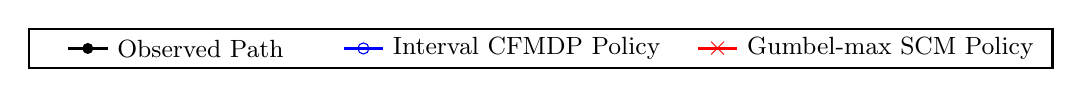
\begin{tikzpicture}[scale=1.0, every node/.style={scale=1.0}]
            \draw[thick, black] (-3, -0.25) rectangle (10, 0.25);
            %
            \draw[black, line width=1pt] (-2.5, 0.0) -- (-2,0.0);
            \fill[black] (-2.25,0.0) circle (2pt); %
            \node[right] at (-2,0.0) {\small Observed Path};
            
            %
            \draw[blue, line width=1pt] (1.0,0.0) -- (1.5,0.0);
            \node[draw=blue, circle, minimum size=4pt, inner sep=0pt] at (1.25,0.0) {}; %
            \node[right] at (1.5,0.0) {\small Interval CFMDP Policy};
            
            %
            \draw[red, line width=1pt] (5.5,0) -- (6,0);
            \node[red] at (5.75,0) {$\boldsymbol{\times}$}; %
            \node[right] at (6,0) {\small Gumbel-max SCM Policy};
        \end{tikzpicture}
    }\\
    %
    \subfigure[\footnotesize Lowest cumulative reward: Interval CFMDP ($312$), Gumbel-max SCM ($312$)]{%
        \resizebox{0.76\columnwidth}{!}{
             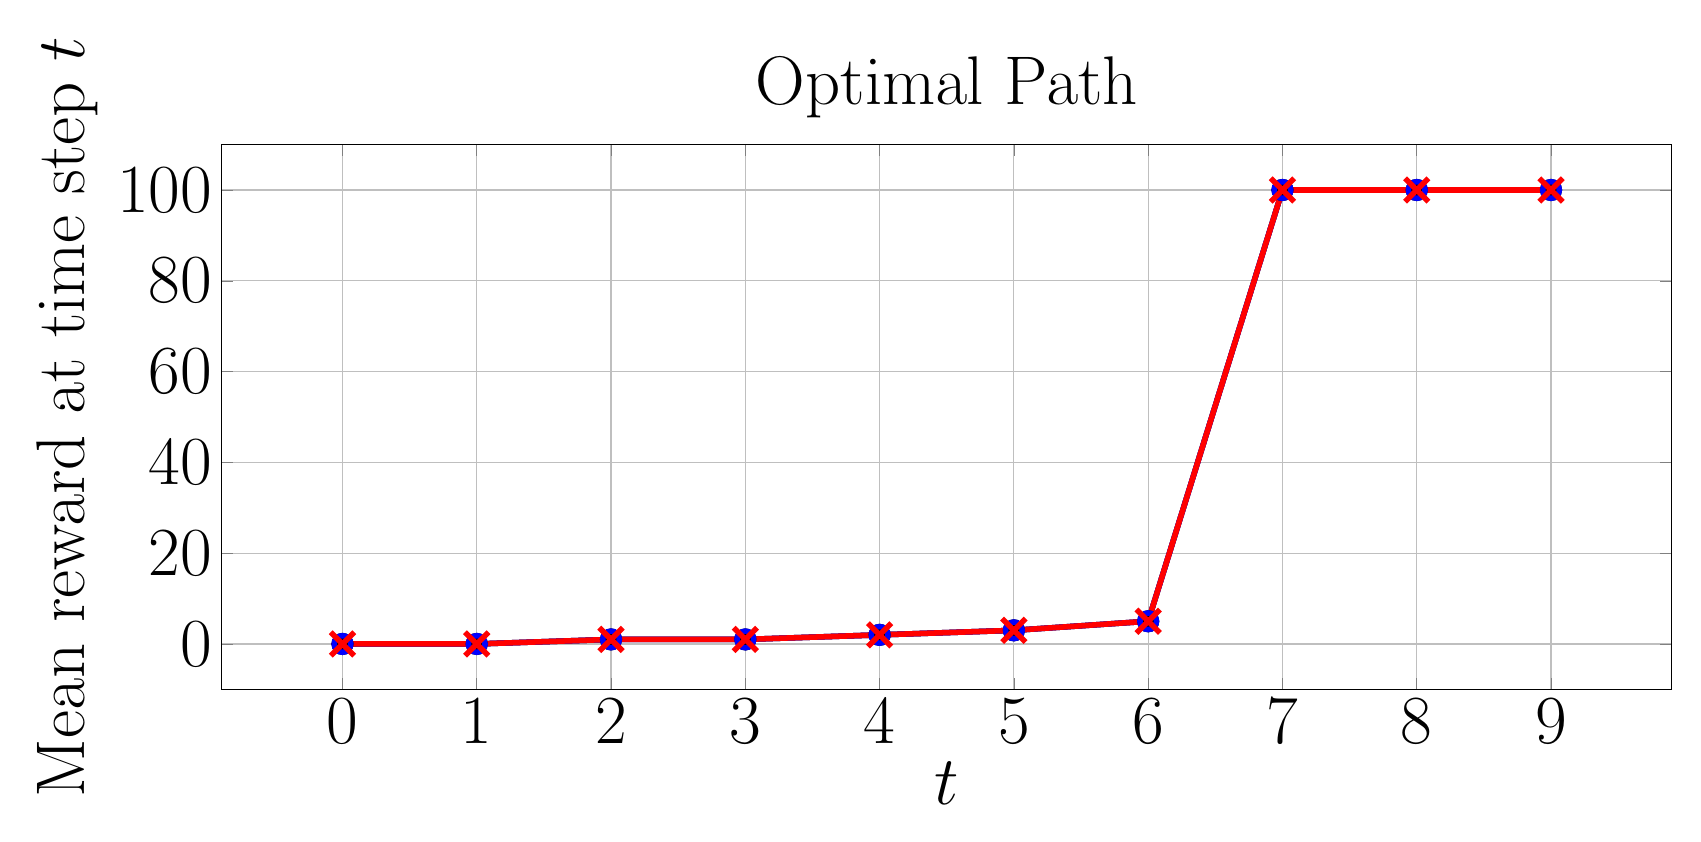
\begin{tikzpicture}
                \begin{axis}[
                    xlabel={$t$},
                    ylabel={Mean reward at time step $t$},
                    title={Optimal Path},
                    grid=both,
                    width=20cm, height=8.5cm,
                    every axis/.style={font=\Huge},
                    %
                ]
                \addplot[
                    color=black, %
                    mark=*, %
                    line width=2pt,
                    mark size=3pt,
                    error bars/.cd,
                    y dir=both, %
                    y explicit, %
                    error bar style={line width=1pt,solid},
                    error mark options={line width=1pt,mark size=4pt,rotate=90}
                ]
                coordinates {
                    (0, 0.0)  +- (0, 0.0)
                    (1, 0.0)  +- (0, 0.0) 
                    (2, 1.0)  +- (0, 0.0) 
                    (3, 1.0)  +- (0, 0.0)
                    (4, 2.0)  +- (0, 0.0)
                    (5, 3.0) +- (0, 0.0)
                    (6, 5.0) +- (0, 0.0)
                    (7, 100.0) +- (0, 0.0)
                    (8, 100.0) +- (0, 0.0)
                    (9, 100.0) +- (0, 0.0)
                };
                %
                \addplot[
                    color=blue, %
                    mark=o, %
                    line width=2pt,
                    mark size=3pt,
                    error bars/.cd,
                    y dir=both, %
                    y explicit, %
                    error bar style={line width=1pt,solid},
                    error mark options={line width=1pt,mark size=4pt,rotate=90}
                ]
                 coordinates {
                    (0, 0.0)  +- (0, 0.0)
                    (1, 0.0)  +- (0, 0.0) 
                    (2, 1.0)  +- (0, 0.0) 
                    (3, 1.0)  +- (0, 0.0)
                    (4, 2.0)  +- (0, 0.0)
                    (5, 3.0) +- (0, 0.0)
                    (6, 5.0) +- (0, 0.0)
                    (7, 100.0) +- (0, 0.0)
                    (8, 100.0) +- (0, 0.0)
                    (9, 100.0) +- (0, 0.0)
                };
                %
                \addplot[
                    color=red, %
                    mark=x, %
                    line width=2pt,
                    mark size=6pt,
                    error bars/.cd,
                    y dir=both, %
                    y explicit, %
                    error bar style={line width=1pt,solid},
                    error mark options={line width=1pt,mark size=4pt,rotate=90}
                ]
                coordinates {
                    (0, 0.0)  +- (0, 0.0)
                    (1, 0.0)  +- (0, 0.0) 
                    (2, 1.0)  +- (0, 0.0) 
                    (3, 1.0)  +- (0, 0.0)
                    (4, 2.0)  +- (0, 0.0)
                    (5, 3.0) +- (0, 0.0)
                    (6, 5.0) +- (0, 0.0)
                    (7, 100.0) +- (0, 0.0)
                    (8, 100.0) +- (0, 0.0)
                    (9, 100.0) +- (0, 0.0)
                };
                \end{axis}
            \end{tikzpicture}
         }
    }
    \hspace{1cm}
    \subfigure[\footnotesize Lowest cumulative reward: Interval CFMDP ($19$), Gumbel-max SCM ($-88$)]{%
         \resizebox{0.76\columnwidth}{!}{
            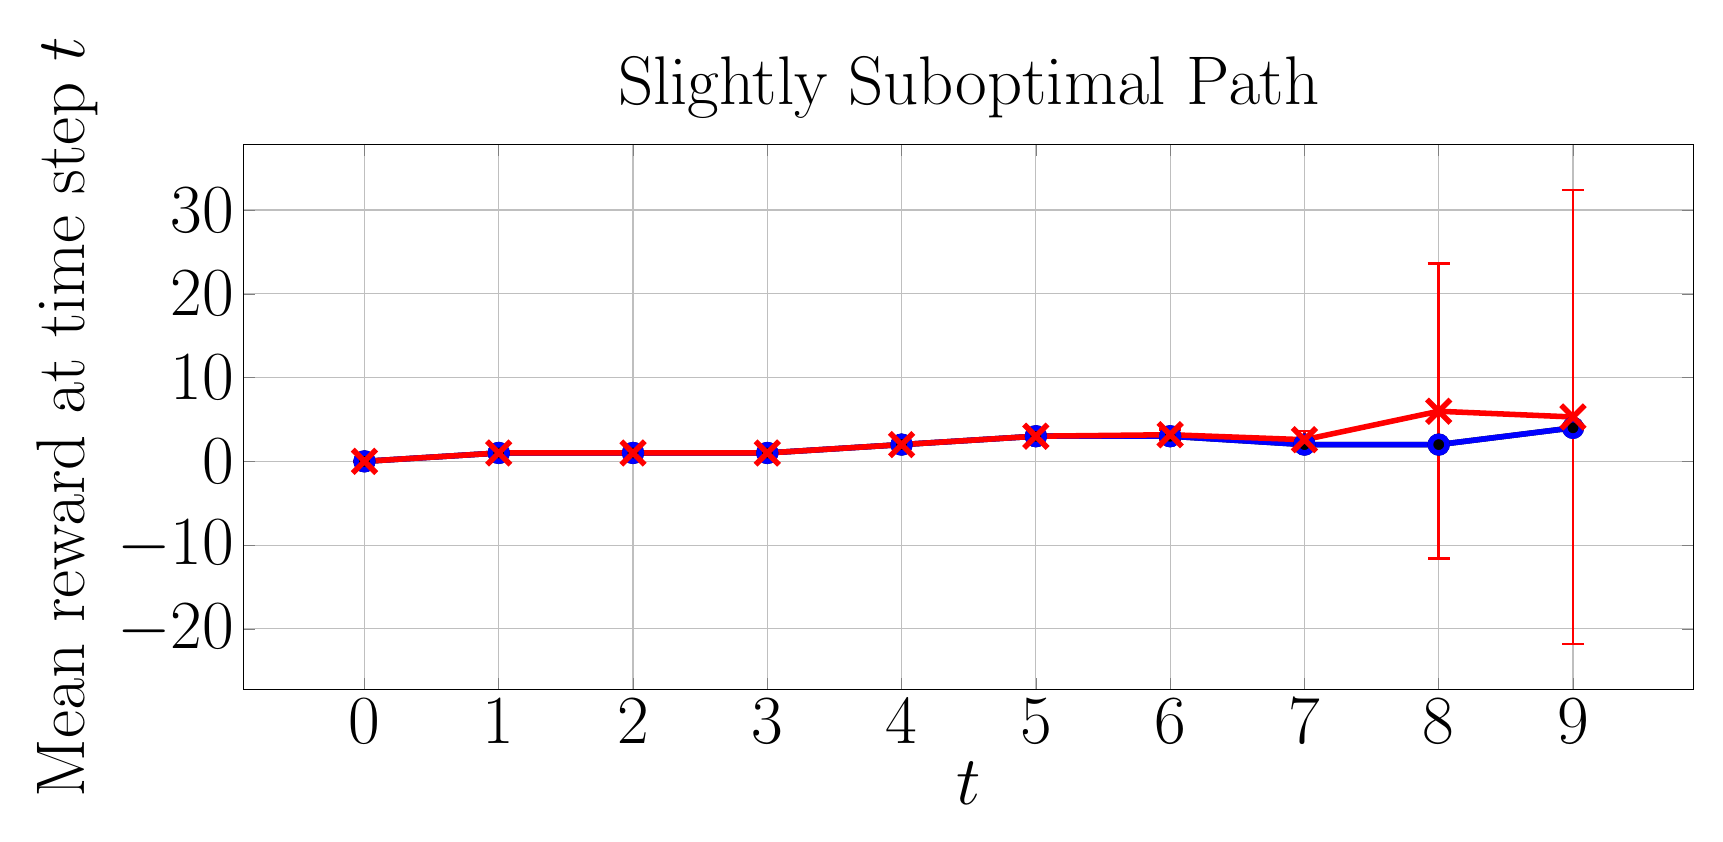
\begin{tikzpicture}
                \begin{axis}[
                    xlabel={$t$},
                    ylabel={Mean reward at time step $t$},
                    title={Slightly Suboptimal Path},
                    grid=both,
                    width=20cm, height=8.5cm,
                    every axis/.style={font=\Huge},
                    %
                ]
                \addplot[
                    color=black, %
                    mark=*, %
                    line width=2pt,
                    mark size=3pt,
                    error bars/.cd,
                    y dir=both, %
                    y explicit, %
                    error bar style={line width=1pt,solid},
                    error mark options={line width=1pt,mark size=4pt,rotate=90}
                ]
              coordinates {
                    (0, 0.0)  +- (0, 0.0)
                    (1, 1.0)  +- (0, 0.0) 
                    (2, 1.0)  +- (0, 0.0) 
                    (3, 1.0)  +- (0, 0.0)
                    (4, 2.0)  +- (0, 0.0)
                    (5, 3.0) +- (0, 0.0)
                    (6, 3.0) +- (0, 0.0)
                    (7, 2.0) +- (0, 0.0)
                    (8, 2.0) +- (0, 0.0)
                    (9, 4.0) +- (0, 0.0)
                };
                %
                \addplot[
                    color=blue, %
                    mark=o, %
                    line width=2pt,
                    mark size=3pt,
                    error bars/.cd,
                    y dir=both, %
                    y explicit, %
                    error bar style={line width=1pt,solid},
                    error mark options={line width=1pt,mark size=4pt,rotate=90}
                ]
              coordinates {
                    (0, 0.0)  +- (0, 0.0)
                    (1, 1.0)  +- (0, 0.0) 
                    (2, 1.0)  +- (0, 0.0) 
                    (3, 1.0)  +- (0, 0.0)
                    (4, 2.0)  +- (0, 0.0)
                    (5, 3.0) +- (0, 0.0)
                    (6, 3.0) +- (0, 0.0)
                    (7, 2.0) +- (0, 0.0)
                    (8, 2.0) +- (0, 0.0)
                    (9, 4.0) +- (0, 0.0)
                };
                %
                \addplot[
                    color=red, %
                    mark=x, %
                    line width=2pt,
                    mark size=6pt,
                    error bars/.cd,
                    y dir=both, %
                    y explicit, %
                    error bar style={line width=1pt,solid},
                    error mark options={line width=1pt,mark size=4pt,rotate=90}
                ]
                coordinates {
                    (0, 0.0)  +- (0, 0.0)
                    (1, 1.0)  +- (0, 0.0) 
                    (2, 1.0)  +- (0, 0.0) 
                    (3, 1.0)  +- (0, 0.0)
                    (4, 2.0)  += (0, 0.0)
                    (5, 3.0)  += (0, 0.0)
                    (6, 3.17847) += (0, 0.62606746) -= (0, 0.62606746)
                    (7, 2.5832885) += (0, 1.04598233) -= (0, 1.04598233)
                    (8, 5.978909) += (0, 17.60137623) -= (0, 17.60137623)
                    (9, 5.297059) += (0, 27.09227512) -= (0, 27.09227512)
                };
                \end{axis}
            \end{tikzpicture}
         }
    }\\[-1.5pt]
    \subfigure[\footnotesize Lowest cumulative reward: Interval CFMDP ($14$), Gumbel-max SCM ($-598$)]{%
         \resizebox{0.76\columnwidth}{!}{
             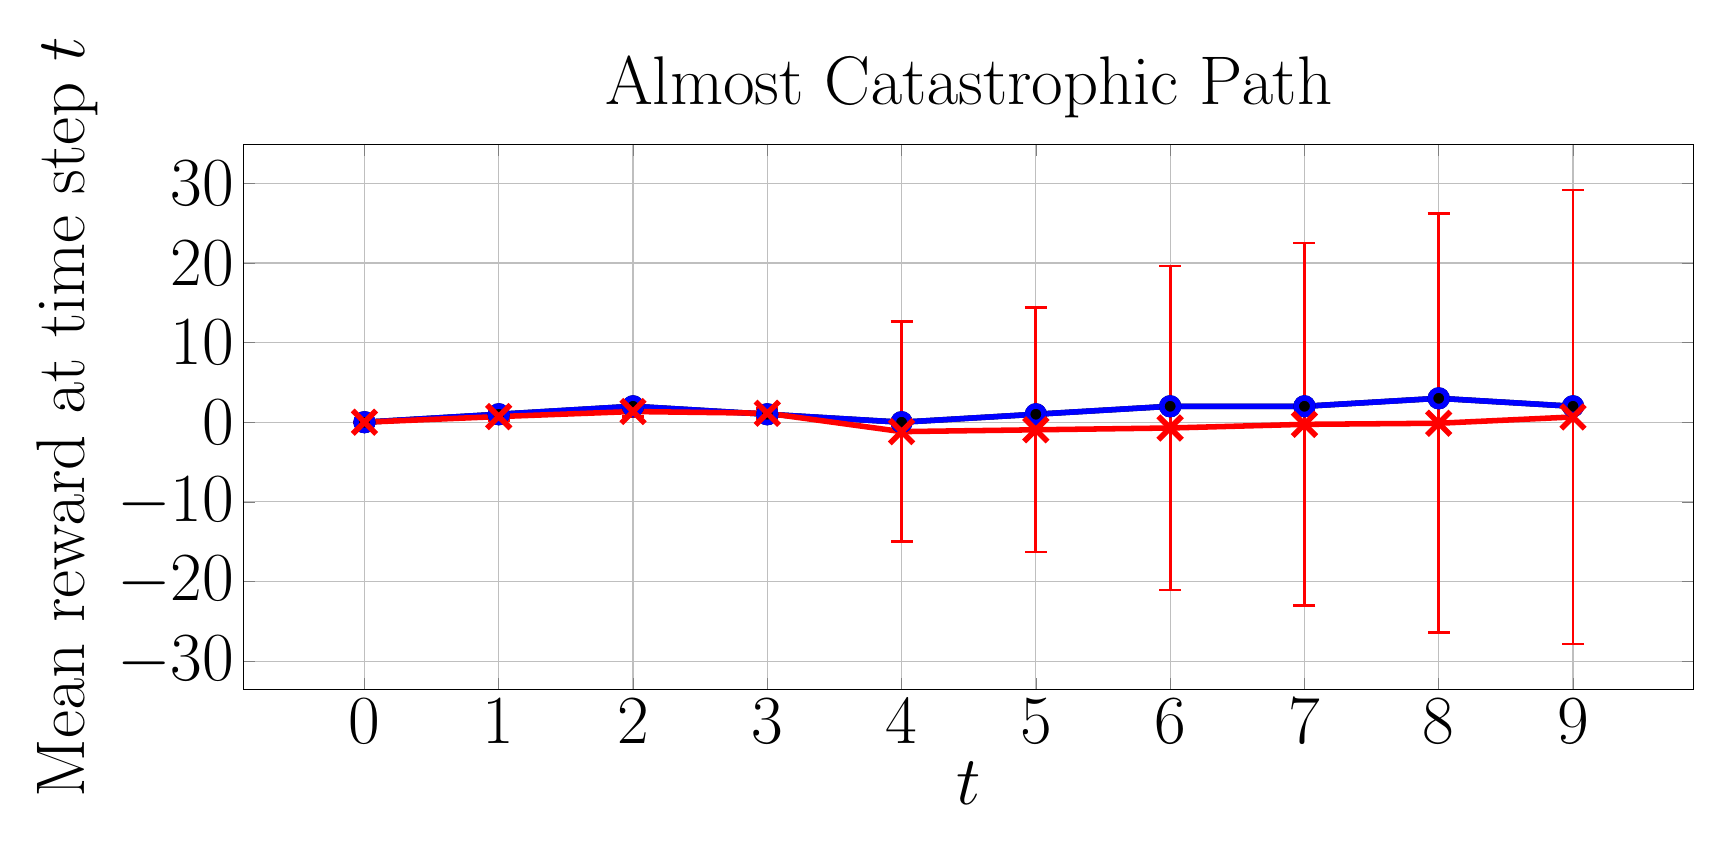
\begin{tikzpicture}
                \begin{axis}[
                    xlabel={$t$},
                    ylabel={Mean reward at time step $t$},
                    title={Almost Catastrophic Path},
                    grid=both,
                    width=20cm, height=8.5cm,
                    every axis/.style={font=\Huge},
                    %
                ]
                \addplot[
                    color=black, %
                    mark=*, %
                    line width=2pt,
                    mark size=3pt,
                    error bars/.cd,
                    y dir=both, %
                    y explicit, %
                    error bar style={line width=1pt,solid},
                    error mark options={line width=1pt,mark size=4pt,rotate=90}
                ]
                coordinates {
                    (0, 0.0)  +- (0, 0.0)
                    (1, 1.0)  +- (0, 0.0) 
                    (2, 2.0)  +- (0, 0.0) 
                    (3, 1.0)  +- (0, 0.0)
                    (4, 0.0)  +- (0, 0.0)
                    (5, 1.0) +- (0, 0.0)
                    (6, 2.0) +- (0, 0.0)
                    (7, 2.0) +- (0, 0.0)
                    (8, 3.0) +- (0, 0.0)
                    (9, 2.0) +- (0, 0.0)
                };
                %
                \addplot[
                    color=blue, %
                    mark=o, %
                    line width=2pt,
                    mark size=3pt,
                    error bars/.cd,
                    y dir=both, %
                    y explicit, %
                    error bar style={line width=1pt,solid},
                    error mark options={line width=1pt,mark size=4pt,rotate=90}
                ]
                coordinates {
                    (0, 0.0)  +- (0, 0.0)
                    (1, 1.0)  +- (0, 0.0) 
                    (2, 2.0)  +- (0, 0.0) 
                    (3, 1.0)  +- (0, 0.0)
                    (4, 0.0)  +- (0, 0.0)
                    (5, 1.0) +- (0, 0.0)
                    (6, 2.0) +- (0, 0.0)
                    (7, 2.0) +- (0, 0.0)
                    (8, 3.0) +- (0, 0.0)
                    (9, 2.0) +- (0, 0.0)
                };
                %
                \addplot[
                    color=red, %
                    mark=x, %
                    line width=2pt,
                    mark size=6pt,
                    error bars/.cd,
                    y dir=both, %
                    y explicit, %
                    error bar style={line width=1pt,solid},
                    error mark options={line width=1pt,mark size=4pt,rotate=90}
                ]
                coordinates {
                    (0, 0.0)  +- (0, 0.0)
                    (1, 0.7065655)  +- (0, 0.4553358) 
                    (2, 1.341673)  +- (0, 0.67091621) 
                    (3, 1.122926)  +- (0, 0.61281824)
                    (4, -1.1821935)  +- (0, 13.82444042)
                    (5, -0.952399)  +- (0, 15.35195457)
                    (6, -0.72672) +- (0, 20.33508414)
                    (7, -0.268983) +- (0, 22.77861454)
                    (8, -0.1310835) +- (0, 26.31013314)
                    (9, 0.65806) +- (0, 28.50670214)
                };
                %
            %
            %
            %
            %
            %
            %
            %
            %
            %
            %
            %
            %
            %
            %
            %
            %
            %
            %
                \end{axis}
            \end{tikzpicture}
         }
    }
    \hspace{1cm}
    \subfigure[\footnotesize Lowest cumulative reward: Interval CFMDP ($-698$), Gumbel-max SCM ($-698$)]{%
         \resizebox{0.76\columnwidth}{!}{
            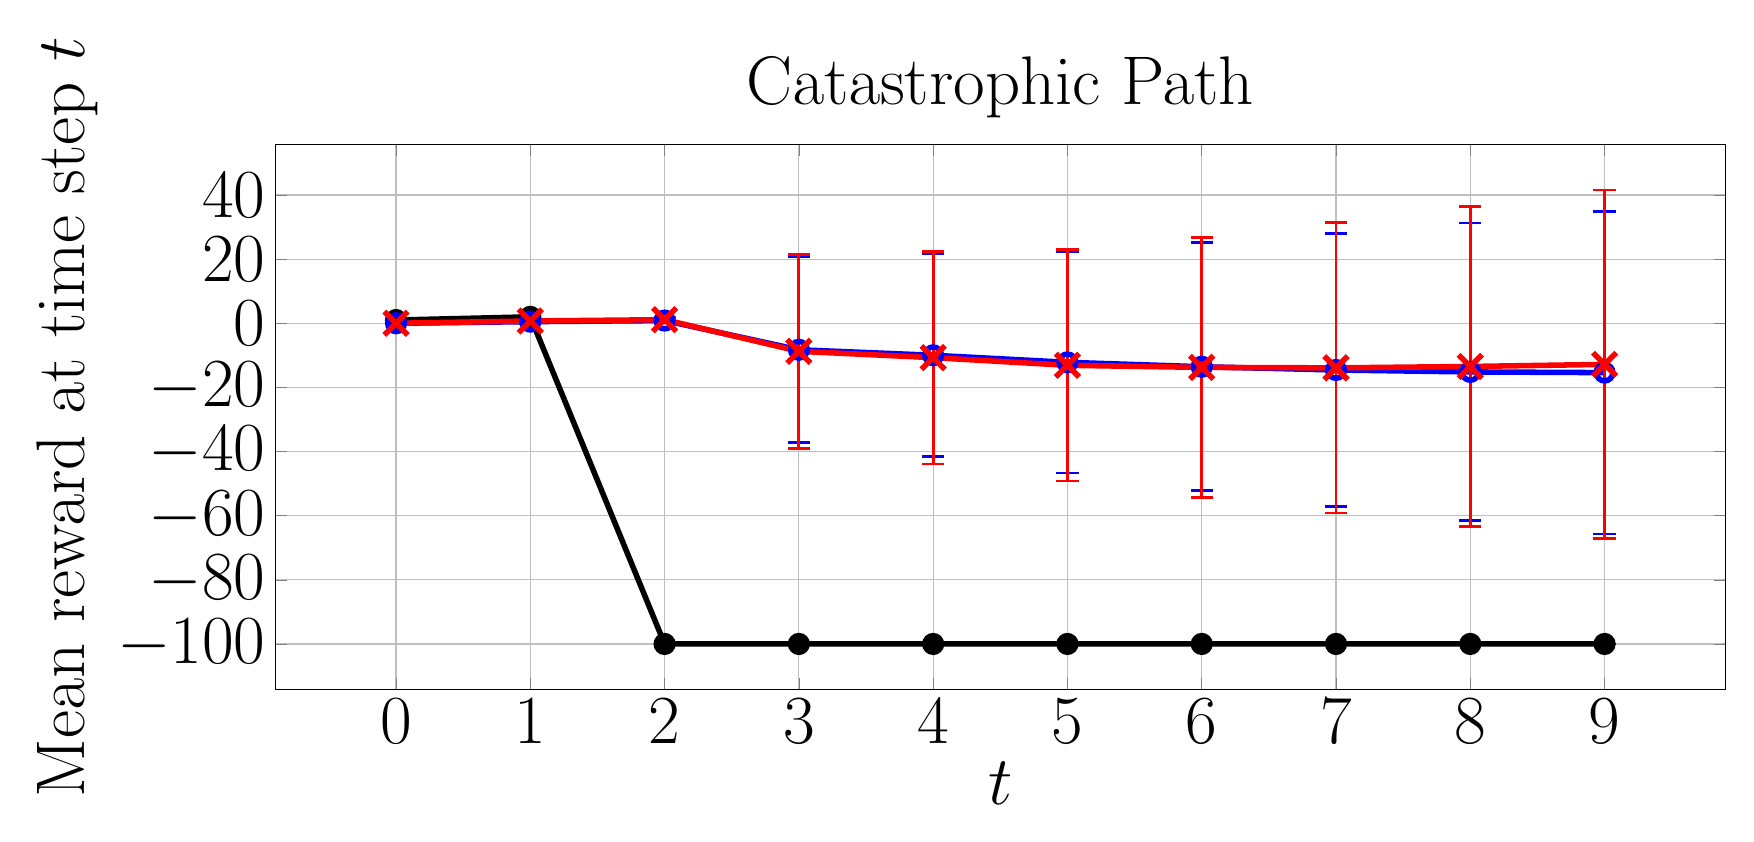
\begin{tikzpicture}
                \begin{axis}[
                    xlabel={$t$},
                    ylabel={Mean reward at time step $t$},
                    title={Catastrophic Path},
                    grid=both,
                    width=20cm, height=8.5cm,
                    every axis/.style={font=\Huge},
                    %
                ]
                \addplot[
                    color=black, %
                    mark=*, %
                    line width=2pt,
                    mark size=3pt,
                    error bars/.cd,
                    y dir=both, %
                    y explicit, %
                    error bar style={line width=1pt,solid},
                    error mark options={line width=1pt,mark size=4pt,rotate=90}
                ]
                coordinates {
                    (0, 1.0)  +- (0, 0.0)
                    (1, 2.0)  +- (0, 0.0) 
                    (2, -100.0)  +- (0, 0.0) 
                    (3, -100.0)  +- (0, 0.0)
                    (4, -100.0)  +- (0, 0.0)
                    (5, -100.0) +- (0, 0.0)
                    (6, -100.0) +- (0, 0.0)
                    (7, -100.0) +- (0, 0.0)
                    (8, -100.0) +- (0, 0.0)
                    (9, -100.0) +- (0, 0.0)
                };
                %
                \addplot[
                    color=blue, %
                    mark=o, %
                    line width=2pt,
                    mark size=3pt,
                    error bars/.cd,
                    y dir=both, %
                    y explicit, %
                    error bar style={line width=1pt,solid},
                    error mark options={line width=1pt,mark size=4pt,rotate=90}
                ]
                coordinates {
                    (0, 0.0)  +- (0, 0.0)
                    (1, 0.504814)  +- (0, 0.49997682) 
                    (2, 0.8439835)  +- (0, 0.76831917) 
                    (3, -8.2709165)  +- (0, 28.93656754)
                    (4, -9.981082)  +- (0, 31.66825363)
                    (5, -12.1776325) +- (0, 34.53463233)
                    (6, -13.556076) +- (0, 38.62845372)
                    (7, -14.574418) +- (0, 42.49603359)
                    (8, -15.1757075) +- (0, 46.41913968)
                    (9, -15.3900395) +- (0, 50.33563368)
                };
                %
                \addplot[
                    color=red, %
                    mark=x, %
                    line width=2pt,
                    mark size=6pt,
                    error bars/.cd,
                    y dir=both, %
                    y explicit, %
                    error bar style={line width=1pt,solid},
                    error mark options={line width=1pt,mark size=4pt,rotate=90}
                ]
                coordinates {
                    (0, 0.0)  +- (0, 0.0)
                    (1, 0.701873)  +- (0, 0.45743556) 
                    (2, 1.1227805)  +- (0, 0.73433129) 
                    (3, -8.7503255)  +- (0, 30.30257976)
                    (4, -10.722092)  +- (0, 33.17618589)
                    (5, -13.10721)  +- (0, 36.0648089)
                    (6, -13.7631645) +- (0, 40.56553451)
                    (7, -13.909043) +- (0, 45.23829402)
                    (8, -13.472517) +- (0, 49.96270296)
                    (9, -12.8278835) +- (0, 54.38618735)
                };
                %
            %
            %
            %
            %
            %
            %
            %
            %
            %
            %
            %
            %
            %
            %
            %
            %
            %
            %
                \end{axis}
            \end{tikzpicture}
         }
    }
    \caption{Average instant reward of CF paths induced by policies on GridWorld $p=0.4$.}
    \label{fig: reward p=0.4}
\end{figure*}

\subsection{Experimental Setup}
To compare policy performance, we measure the average rewards of counterfactual paths induced by our policy and the Gumbel-max policy by uniformly sampling $200$ counterfactual MDPs from the ICFMDP and generating $10,000$ counterfactual paths over each sampled CFMDP. \jl{Since the interval CFMDP depends on the observed path, we select $4$  paths of varying optimality to evaluate how the observed path impacts the performance of both policies: an optimal path, a slightly suboptimal path that could reach the optimal reward with a few changes, a catastrophic path that enters a catastrophic, terminal state with low reward, and an almost catastrophic path that was close to entering a catastrophic state.} When measuring the average probability bound widths and execution time needed to generate the ICFMDPs, we averaged over $20$ randomly generated observed paths
\footnote{Further training details are provided in Appendix \ref{app: training details}, and the code is provided at \href{https://github.com/ddv-lab/robust-cf-inference-in-MDPs}{https://github.com/ddv-lab/robust-cf-inference-in-MDPs}
%
%
.}.

\subsection{GridWorld}
\jl{The GridWorld MDP is a $4 \times 4$ grid where an agent must navigate from the top-left corner to the goal state in the bottom-right corner, avoiding a dangerous terminal state in the centre. At each time step, the agent can move up, down, left, or right, but there is a small probability (controlled by hyper-parameter $p$) of moving in an unintended direction. As the agent nears the goal, the reward for each state increases, culminating in a reward of $+100$ for reaching the goal. Entering the dangerous state results in a penalty of $-100$. We use two versions of GridWorld: a less stochastic version with $p=0.9$ (i.e., $90$\% chance of moving in the chosen direction) and a more stochastic version with $p=0.4$.}

\paragraph{GridWorld ($p=0.9$)}
When $p=0.9$, the counterfactual probability bounds are typically narrow (see Table \ref{tab:nonzero_probs} for average measurements). Consequently, as shown in Figure \ref{fig: reward p=0.9}, both policies are nearly identical and perform similarly well across the optimal, slightly suboptimal, and catastrophic paths.
%
However, for the almost catastrophic path, the interval CFMDP path is more conservative and follows the observed path more closely (as this is where the probability bounds are narrowest), which typically requires one additional step to reach the goal state than the Gumbel-max SCM policy.
%

\paragraph{GridWorld ($p=0.4$)}
\jl{When $p=0.4$, the GridWorld environment becomes more uncertain, increasing the risk of entering the dangerous state even if correct actions are chosen. Thus, as shown in Figure \ref{fig: reward p=0.4}, the interval CFMDP policy adopts a more conservative approach, avoiding deviation from the observed policy if it cannot guarantee higher counterfactual rewards (see the slightly suboptimal and almost catastrophic paths), whereas the Gumbel-max SCM is inconsistent: it can yield higher rewards, but also much lower rewards, reflected in the wide error bars.} For the catastrophic path, both policies must deviate from the observed path to achieve a higher reward and, in this case, perform similarly.
%
%
%
%
\subsection{Sepsis}
The Sepsis MDP \citep{oberst2019counterfactual} simulates trajectories of Sepsis patients. Each state consists of four vital signs (heart rate, blood pressure, oxygen concentration, and glucose levels), categorised as low, normal, or high.
and three treatments that can be toggled on/off at each time step (8 actions in total). Unlike \citet{oberst2019counterfactual}, we scale rewards based on the number of out-of-range vital signs, between $-1000$ (patient dies) and $1000$ (patient discharged). \jl{Like the GridWorld $p=0.4$ experiment, the Sepsis MDP is highly uncertain, as many states are equally likely to lead to optimal and poor outcomes. Thus, as shown in Figure \ref{fig: reward sepsis}, both policies follow the observed optimal and almost catastrophic paths to guarantee rewards are no worse than the observation.} However, improving the catastrophic path requires deviating from the observation. Here, the Gumbel-max SCM policy, on average, performs better than the interval CFMDP policy. But, since both policies have lower bounds clipped at $-1000$, neither policy reliably improves over the observation. In contrast, for the slightly suboptimal path, the interval CFMDP policy performs significantly better, shown by its higher lower bounds. 
Moreover, in these two cases, the worst-case counterfactual path generated by the interval CFMDP policy is better than that of the Gumbel-max SCM policy,
indicating its greater robustness.
%
\begin{figure*}
    \centering
     \resizebox{0.6\textwidth}{!}{
        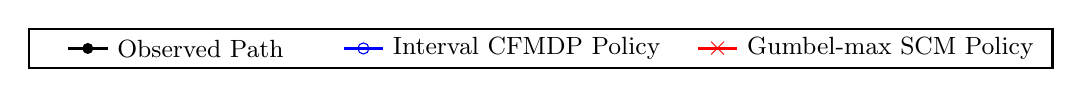
\begin{tikzpicture}[scale=1.0, every node/.style={scale=1.0}]
            \draw[thick, black] (-3, -0.25) rectangle (10, 0.25);
            %
            \draw[black, line width=1pt] (-2.5, 0.0) -- (-2,0.0);
            \fill[black] (-2.25,0.0) circle (2pt); %
            \node[right] at (-2,0.0) {\small Observed Path};
            
            %
            \draw[blue, line width=1pt] (1.0,0.0) -- (1.5,0.0);
            \node[draw=blue, circle, minimum size=4pt, inner sep=0pt] at (1.25,0.0) {}; %
            \node[right] at (1.5,0.0) {\small Interval CFMDP Policy};
            
            %
            \draw[red, line width=1pt] (5.5,0) -- (6,0);
            \node[red] at (5.75,0) {$\boldsymbol{\times}$}; %
            \node[right] at (6,0) {\small Gumbel-max SCM Policy};
        \end{tikzpicture}
    }\\
    \subfigure[\footnotesize Lowest cumulative reward: Interval CFMDP ($8000$), Gumbel-max SCM ($8000$)]{%
         \resizebox{0.76\columnwidth}{!}{
             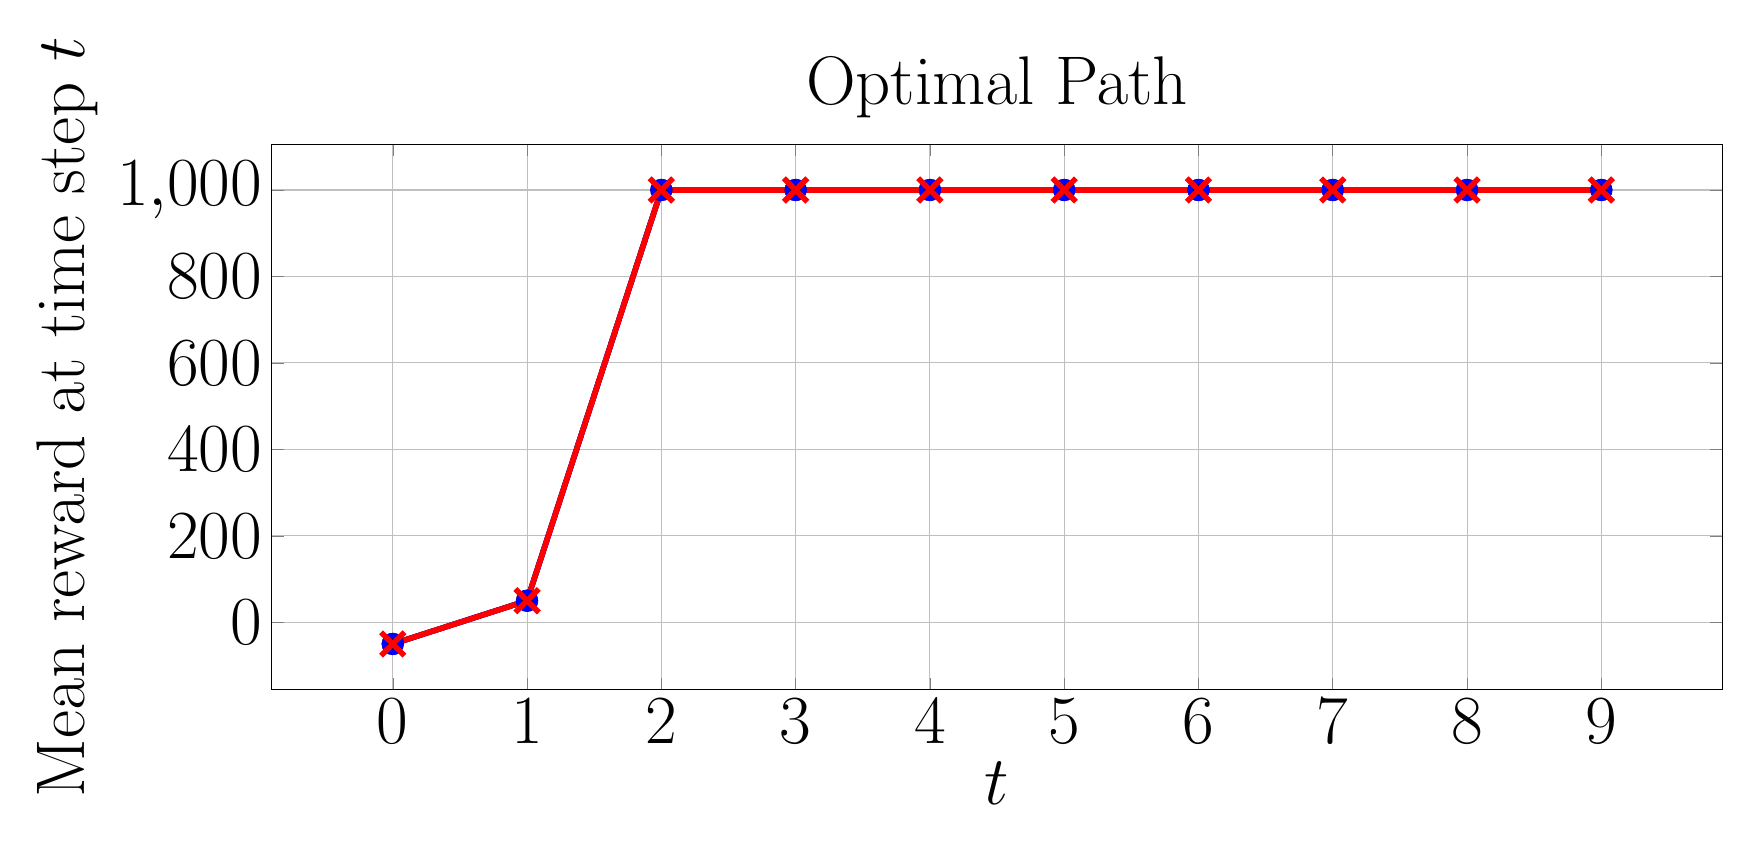
\begin{tikzpicture}
                \begin{axis}[
                    xlabel={$t$},
                    ylabel={Mean reward at time step $t$},
                    title={Optimal Path},
                    grid=both,
                    width=20cm, height=8.5cm,
                    every axis/.style={font=\Huge},
                    %
                ]
                \addplot[
                    color=black, %
                    mark=*, %
                    line width=2pt,
                    mark size=3pt,
                ]
                coordinates {
                    (0, -50.0)
                    (1, 50.0)
                    (2, 1000.0)
                    (3, 1000.0)
                    (4, 1000.0)
                    (5, 1000.0)
                    (6, 1000.0)
                    (7, 1000.0)
                    (8, 1000.0)
                    (9, 1000.0)
                };
                %
                \addplot[
                    color=blue, %
                    mark=o, %
                    line width=2pt,
                    mark size=3pt,
                    error bars/.cd,
                    y dir=both, %
                    y explicit, %
                    error bar style={line width=1pt,solid},
                    error mark options={line width=1pt,mark size=4pt,rotate=90}
                ]
                coordinates {
                    (0, -50.0)  +- (0, 0.0)
                    (1, 50.0)  +- (0, 0.0) 
                    (2, 1000.0)  +- (0, 0.0) 
                    (3, 1000.0)  +- (0, 0.0)
                    (4, 1000.0)  +- (0, 0.0)
                    (5, 1000.0) +- (0, 0.0)
                    (6, 1000.0) +- (0, 0.0)
                    (7, 1000.0) +- (0, 0.0)
                    (8, 1000.0) +- (0, 0.0)
                    (9, 1000.0) +- (0, 0.0)
                };
                %
                \addplot[
                    color=red, %
                    mark=x, %
                    line width=2pt,
                    mark size=6pt,
                    error bars/.cd,
                    y dir=both, %
                    y explicit, %
                    error bar style={line width=1pt,solid},
                    error mark options={line width=1pt,mark size=4pt,rotate=90}
                ]
                coordinates {
                    (0, -50.0)  +- (0, 0.0)
                    (1, 50.0)  +- (0, 0.0) 
                    (2, 1000.0)  +- (0, 0.0) 
                    (3, 1000.0)  +- (0, 0.0)
                    (4, 1000.0)  +- (0, 0.0)
                    (5, 1000.0) +- (0, 0.0)
                    (6, 1000.0) +- (0, 0.0)
                    (7, 1000.0) +- (0, 0.0)
                    (8, 1000.0) +- (0, 0.0)
                    (9, 1000.0) +- (0, 0.0)
                };
                %
                \end{axis}
            \end{tikzpicture}
         }
    }
    \hspace{1cm}
    \subfigure[\footnotesize Lowest cumulative reward: Interval CFMDP ($-5980$), Gumbel-max SCM ($-8000$)]{%
         \resizebox{0.76\columnwidth}{!}{
            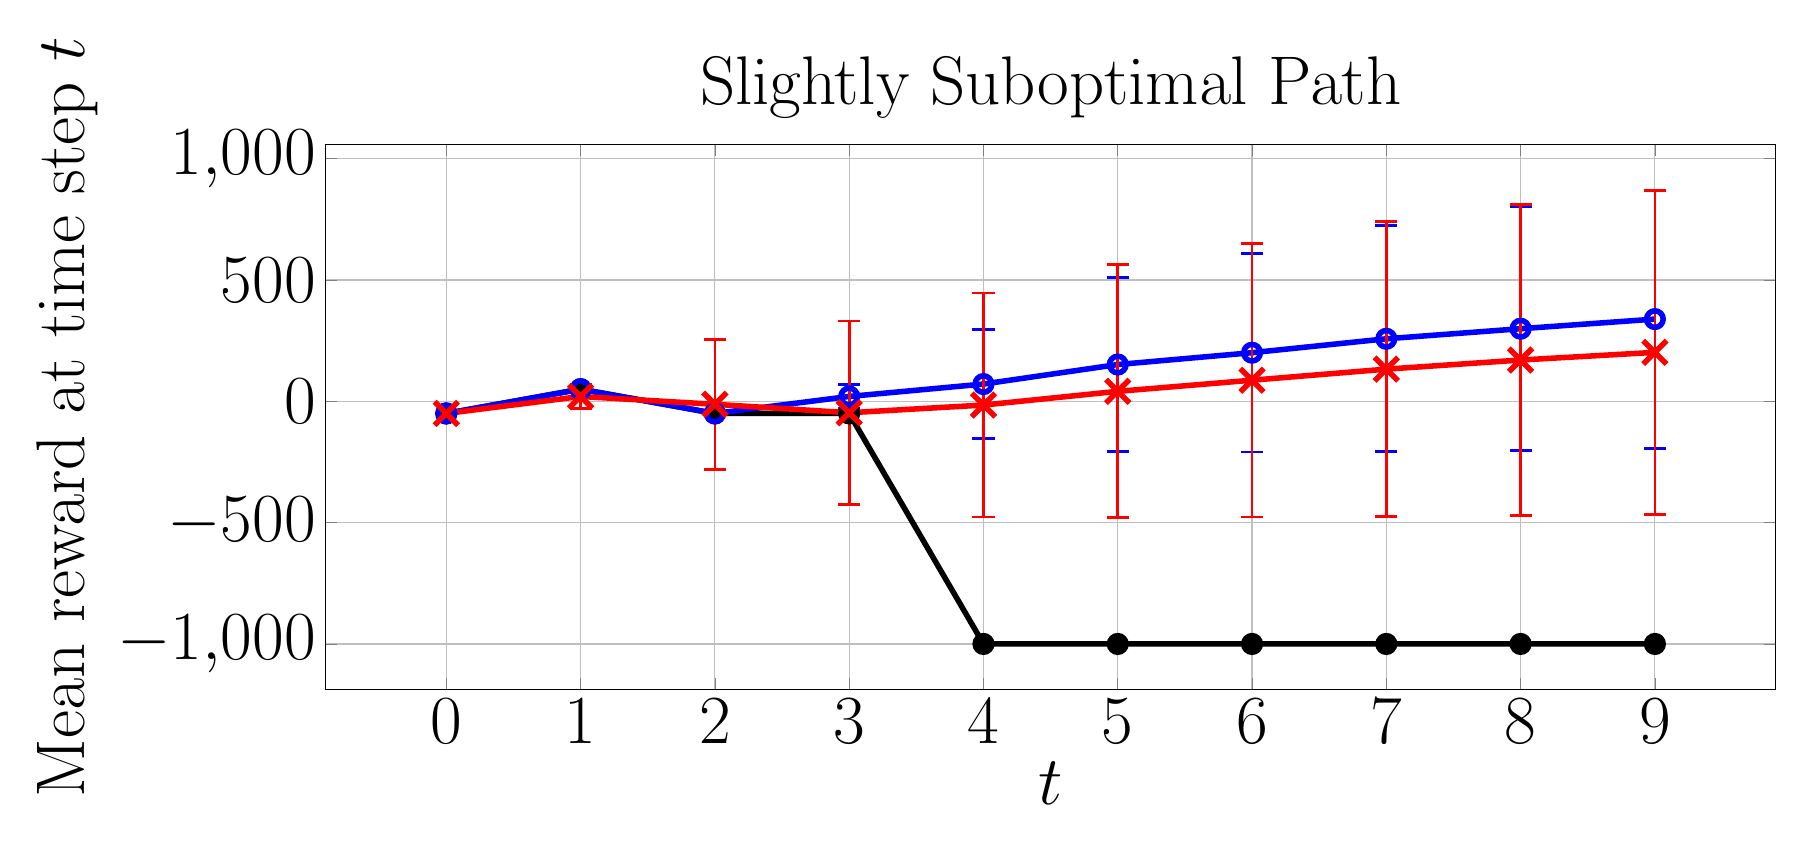
\begin{tikzpicture}
                \begin{axis}[
                    xlabel={$t$},
                    ylabel={Mean reward at time step $t$},
                    title={Slightly Suboptimal Path},
                    grid=both,
                    width=20cm, height=8.5cm,
                    every axis/.style={font=\Huge},
                    %
                ]
               \addplot[
                    color=black, %
                    mark=*, %
                    line width=2pt,
                    mark size=3pt,
                ]
                coordinates {
                    (0, -50.0)
                    (1, 50.0)
                    (2, -50.0)
                    (3, -50.0)
                    (4, -1000.0)
                    (5, -1000.0)
                    (6, -1000.0)
                    (7, -1000.0)
                    (8, -1000.0)
                    (9, -1000.0)
                };
                %
                \addplot[
                    color=blue, %
                    mark=o, %
                    line width=2pt,
                    mark size=3pt,
                    error bars/.cd,
                    y dir=both, %
                    y explicit, %
                    error bar style={line width=1pt,solid},
                    error mark options={line width=1pt,mark size=4pt,rotate=90}
                ]
                coordinates {
                    (0, -50.0)  +- (0, 0.0)
                    (1, 50.0)  +- (0, 0.0) 
                    (2, -50.0)  +- (0, 0.0) 
                    (3, 20.0631)  +- (0, 49.97539413)
                    (4, 71.206585)  +- (0, 226.02033693)
                    (5, 151.60797) +- (0, 359.23292559)
                    (6, 200.40593) +- (0, 408.86185176)
                    (7, 257.77948) +- (0, 466.10372804)
                    (8, 299.237465) +- (0, 501.82579506)
                    (9, 338.9129) +- (0, 532.06124996)
                };
                %
                \addplot[
                    color=red, %
                    mark=x, %
                    line width=2pt,
                    mark size=6pt,
                    error bars/.cd,
                    y dir=both, %
                    y explicit, %
                    error bar style={line width=1pt,solid},
                    error mark options={line width=1pt,mark size=4pt,rotate=90}
                ]
                coordinates {
                    (0, -50.0)  +- (0, 0.0)
                    (1, 20.00736)  +- (0, 49.99786741) 
                    (2, -12.282865)  +- (0, 267.598755) 
                    (3, -47.125995)  +- (0, 378.41755832)
                    (4, -15.381965)  +- (0, 461.77616558)
                    (5, 41.15459) +- (0, 521.53189262)
                    (6, 87.01595) +- (0, 564.22243126 )
                    (7, 132.62376) +- (0, 607.31338037)
                    (8, 170.168145) +- (0, 641.48013693)
                    (9, 201.813135) +- (0, 667.29441777)
                };
                %
                %
                %
                %
                %
                %
                %
                %
                %
                %
                %
                %
                %
                %
                %
                %
                %
                %
                %
                \end{axis}
            \end{tikzpicture}
         }
    }\\[-1.5pt]
    \subfigure[\footnotesize Lowest cumulative reward: Interval CFMDP ($100$), Gumbel-max SCM ($100$)]{%
         \resizebox{0.76\columnwidth}{!}{
             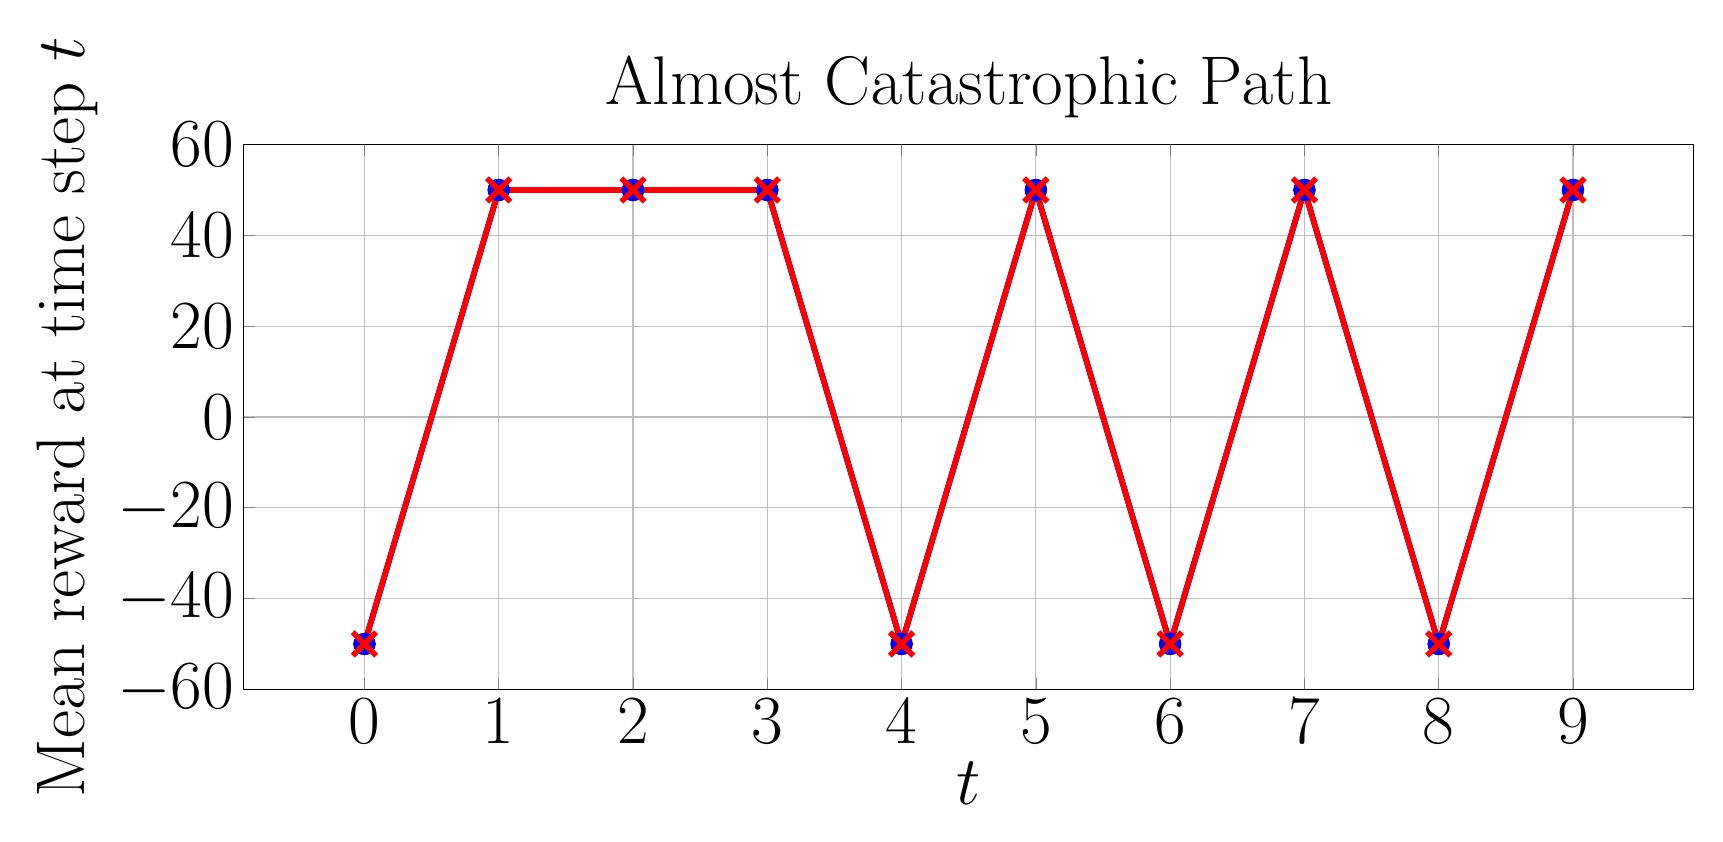
\begin{tikzpicture}
                \begin{axis}[
                    xlabel={$t$},
                    ylabel={Mean reward at time step $t$},
                    title={Almost Catastrophic Path},
                    grid=both,
                    every axis/.style={font=\Huge},
                    width=20cm, height=8.5cm,
                    %
                ]
               \addplot[
                    color=black, %
                    mark=*, %
                    line width=2pt,
                    mark size=3pt,
                ]
                coordinates {
                    (0, -50.0)
                    (1, 50.0)
                    (2, 50.0)
                    (3, 50.0)
                    (4, -50.0)
                    (5, 50.0)
                    (6, -50.0)
                    (7, 50.0)
                    (8, -50.0)
                    (9, 50.0)
                };
                %
                %
                \addplot[
                    color=blue, %
                    mark=o, %
                    line width=2pt,
                    mark size=3pt,
                    error bars/.cd,
                    y dir=both, %
                    y explicit, %
                    error bar style={line width=1pt,solid},
                    error mark options={line width=1pt,mark size=4pt,rotate=90}
                ]
                coordinates {
                    (0, -50.0)  +- (0, 0.0)
                    (1, 50.0)  +- (0, 0.0) 
                    (2, 50.0)  +- (0, 0.0) 
                    (3, 50.0)  +- (0, 0.0)
                    (4, -50.0)  +- (0, 0.0)
                    (5, 50.0) +- (0, 0.0)
                    (6, -50.0) +- (0, 0.0)
                    (7, 50.0) +- (0, 0.0)
                    (8, -50.0) +- (0, 0.0)
                    (9, 50.0) +- (0, 0.0)
                };
                %
                \addplot[
                    color=red, %
                    mark=x, %
                    line width=2pt,
                    mark size=6pt,
                    error bars/.cd,
                    y dir=both, %
                    y explicit, %
                    error bar style={line width=1pt,solid},
                    error mark options={line width=1pt,mark size=4pt,rotate=90}
                ]
                coordinates {
                    (0, -50.0)  +- (0, 0.0)
                    (1, 50.0)  +- (0, 0.0) 
                    (2, 50.0)  +- (0, 0.0) 
                    (3, 50.0)  +- (0, 0.0)
                    (4, -50.0)  +- (0, 0.0)
                    (5, 50.0) +- (0, 0.0)
                    (6, -50.0) +- (0, 0.0)
                    (7, 50.0) +- (0, 0.0)
                    (8, -50.0) +- (0, 0.0)
                    (9, 50.0) +- (0, 0.0)
                };
                %
                %
                %
                %
                %
                %
                %
                %
                %
                %
                %
                %
                %
                %
                %
                %
                %
                %
                %
                \end{axis}
            \end{tikzpicture}
         }
    }
    \hspace{1cm}
    \subfigure[\footnotesize Lowest cumulative reward: Interval CFMDP ($-7150$), Gumbel-max SCM ($-9050$)]{%
         \resizebox{0.76\columnwidth}{!}{
            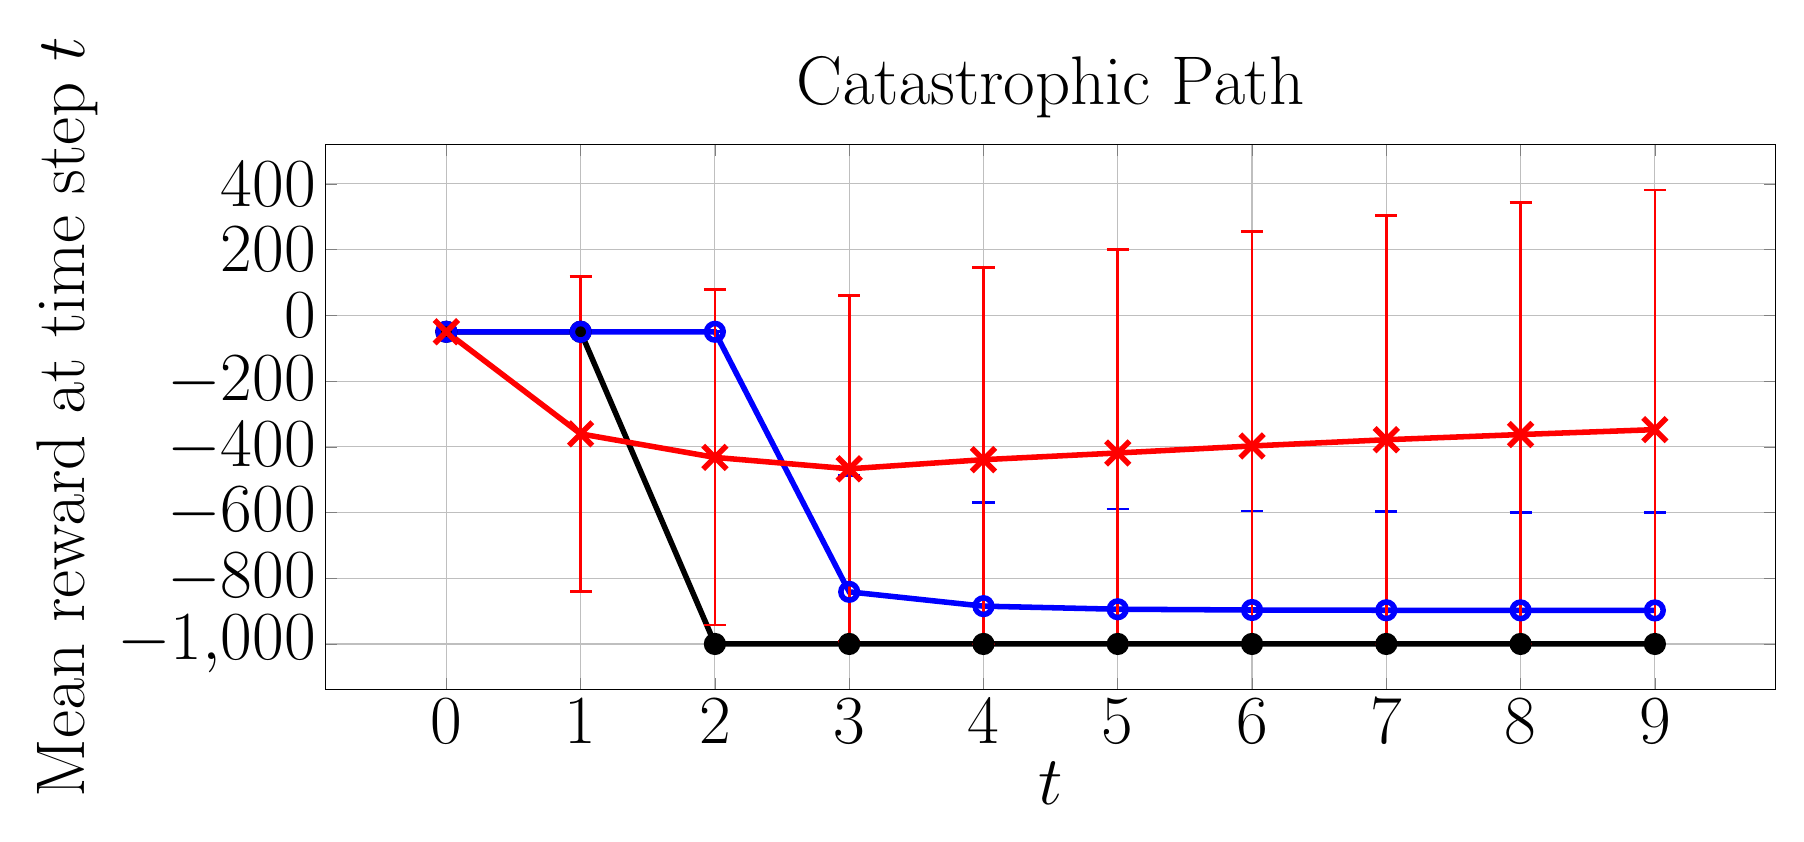
\begin{tikzpicture}
                \begin{axis}[
                    xlabel={$t$},
                    ylabel={Mean reward at time step $t$},
                    title={Catastrophic Path},
                    grid=both,
                    width=20cm, height=8.5cm,
                    every axis/.style={font=\Huge},
                    %
                ]
               \addplot[
                    color=black, %
                    mark=*, %
                    line width=2pt,
                    mark size=3pt,
                ]
                coordinates {
                    (0, -50.0)
                    (1, -50.0)
                    (2, -1000.0)
                    (3, -1000.0)
                    (4, -1000.0)
                    (5, -1000.0)
                    (6, -1000.0)
                    (7, -1000.0)
                    (8, -1000.0)
                    (9, -1000.0)
                };
                %
                %
                \addplot[
                    color=blue, %
                    mark=o, %
                    line width=2pt,
                    mark size=3pt,
                    error bars/.cd,
                    y dir=both, %
                    y explicit, %
                    error bar style={line width=1pt,solid},
                    error mark options={line width=1pt,mark size=4pt,rotate=90}
                ]
                coordinates {
                    (0, -50.0)  +- (0, 0.0)
                    (1, -50.0)  +- (0, 0.0) 
                    (2, -50.0)  +- (0, 0.0) 
                    (3, -841.440725)  += (0, 354.24605512) -= (0, 158.559275)
                    (4, -884.98225)  += (0, 315.37519669) -= (0, 115.01775)
                    (5, -894.330425) += (0, 304.88572805) -= (0, 105.669575)
                    (6, -896.696175) += (0, 301.19954514) -= (0, 103.303825)
                    (7, -897.4635) += (0, 299.61791279) -= (0, 102.5365)
                    (8, -897.77595) += (0, 298.80392585) -= (0, 102.22405)
                    (9, -897.942975) += (0, 298.32920557) -= (0, 102.057025)
                };
                %
                \addplot[
                    color=red, %
                    mark=x, %
                    line width=2pt,
                    mark size=6pt,
                    error bars/.cd,
                    y dir=both, %
                    y explicit, %
                    error bar style={line width=1pt,solid},
                    error mark options={line width=1pt,mark size=4pt,rotate=90}
                ]
            coordinates {
                    (0, -50.0)  +- (0, 0.0)
                    (1, -360.675265)  +- (0, 479.39812699) 
                    (2, -432.27629)  +- (0, 510.38620897) 
                    (3, -467.029545)  += (0, 526.36009628) -= (0, 526.36009628)
                    (4, -439.17429)  += (0, 583.96638919) -= (0, 560.82571)
                    (5, -418.82704) += (0, 618.43027478) -= (0, 581.17296)
                    (6, -397.464895) += (0, 652.67322574) -= (0, 602.535105)
                    (7, -378.49052) += (0, 682.85407033) -= (0, 621.50948)
                    (8, -362.654195) += (0, 707.01412023) -= (0, 637.345805)
                    (9, -347.737935) += (0, 729.29076479) -= (0, 652.262065)
                };
                %
                %
                %
                %
                %
                %
                %
                %
                %
                %
                %
                %
                %
                %
                %
                %
                %
                %
                %
                \end{axis}
            \end{tikzpicture}
         }
    }
    \caption{Average instant reward of CF paths induced by policies on Sepsis.}
    \label{fig: reward sepsis}
\end{figure*}

%
%
%
\subsection{Interval CFMDP Bounds}
%
%
Table \ref{tab:nonzero_probs} presents the mean counterfactual probability bound widths (excluding transitions where the upper bound is $0$) for each MDP, averaged over 20 observed paths. We compare the bounds under counterfactual stability (CS) and monotonicity (M) assumptions, CS alone, and no assumptions. This shows that the assumptions marginally reduce the bound widths, indicating the assumptions tighten the bounds without excluding too many causal models, as intended.
\renewcommand{\arraystretch}{1}

\begin{table}
\centering
\caption{Mean width of counterfactual probability bounds}
\resizebox{0.8\columnwidth}{!}{%
\begin{tabular}{|c|c|c|c|}
\hline
\multirow{2}{*}{\textbf{Environment}} & \multicolumn{3}{c|}{\textbf{Assumptions}} \\ \cline{2-4}
 & \textbf{CS + M} & \textbf{CS} & \textbf{None\tablefootnote{\jl{Equivalent to \citet{li2024probabilities}'s bounds (see Section \ref{sec: equivalence with Li}).}}} \\ \hline
\textbf{GridWorld} ($p=0.9$) & 0.0817 & 0.0977 & 0.100 \\ \hline
\textbf{GridWorld} ($p=0.4$) & 0.552  & 0.638  & 0.646 \\ \hline
\textbf{Sepsis} & 0.138 & 0.140 & 0.140 \\ \hline
\end{tabular}
}
\label{tab:nonzero_probs}
\end{table}


\subsection{Execution Times}
Table \ref{tab: times} compares the average time needed to generate the interval CFMDP vs.\ the Gumbel-max SCM CFMDP for 20 observations.
The GridWorld algorithms were run single-threaded, while the Sepsis experiments were run in parallel.
Generating the interval CFMDP is significantly faster as it uses exact analytical bounds, whereas the Gumbel-max CFMDP requires sampling from the Gumbel distribution to estimate counterfactual transition probabilities. \jl{Since constructing the counterfactual MDP models is the main bottleneck in both approaches, ours is more efficient overall and suitable for larger MDPs.}
\begin{table}
\centering
\caption{Mean execution time to generate CFMDPs}
\resizebox{0.99\columnwidth}{!}{%
\begin{tabular}{|c|c|c|}
\hline
\multirow{2}{*}{\textbf{Environment}} & \multicolumn{2}{c|}{\textbf{Mean Execution Time (s)}} \\ \cline{2-3} 
                                      & \textbf{Interval CFMDP} & \textbf{Gumbel-max CFMDP} \\ \hline
\textbf{GridWorld ($p=0.9$) }                  & 0.261                   & 56.1                      \\ \hline
\textbf{GridWorld ($p=0.4$)  }                 & 0.336                   & 54.5                      \\ \hline
\textbf{Sepsis}                                 & 688                     & 2940                      \\ \hline
\end{tabular}%
}
\label{tab: times}
\end{table}

% \putsec{related}{Related Work}

\noindent \textbf{Efficient Radiance Field Rendering.}
%
The introduction of Neural Radiance Fields (NeRF)~\cite{mil:sri20} has
generated significant interest in efficient 3D scene representation and
rendering for radiance fields.
%
Over the past years, there has been a large amount of research aimed at
accelerating NeRFs through algorithmic or software
optimizations~\cite{mul:eva22,fri:yu22,che:fun23,sun:sun22}, and the
development of hardware
accelerators~\cite{lee:cho23,li:li23,son:wen23,mub:kan23,fen:liu24}.
%
The state-of-the-art method, 3D Gaussian splatting~\cite{ker:kop23}, has
further fueled interest in accelerating radiance field
rendering~\cite{rad:ste24,lee:lee24,nie:stu24,lee:rho24,ham:mel24} as it
employs rasterization primitives that can be rendered much faster than NeRFs.
%
However, previous research focused on software graphics rendering on
programmable cores or building dedicated hardware accelerators. In contrast,
\name{} investigates the potential of efficient radiance field rendering while
utilizing fixed-function units in graphics hardware.
%
To our knowledge, this is the first work that assesses the performance
implications of rendering Gaussian-based radiance fields on the hardware
graphics pipeline with software and hardware optimizations.

%%%%%%%%%%%%%%%%%%%%%%%%%%%%%%%%%%%%%%%%%%%%%%%%%%%%%%%%%%%%%%%%%%%%%%%%%%
\myparagraph{Enhancing Graphics Rendering Hardware.}
%
The performance advantage of executing graphics rendering on either
programmable shader cores or fixed-function units varies depending on the
rendering methods and hardware designs.
%
Previous studies have explored the performance implication of graphics hardware
design by developing simulation infrastructures for graphics
workloads~\cite{bar:gon06,gub:aam19,tin:sax23,arn:par13}.
%
Additionally, several studies have aimed to improve the performance of
special-purpose hardware such as ray tracing units in graphics
hardware~\cite{cho:now23,liu:cha21} and proposed hardware accelerators for
graphics applications~\cite{lu:hua17,ram:gri09}.
%
In contrast to these works, which primarily evaluate traditional graphics
workloads, our work focuses on improving the performance of volume rendering
workloads, such as Gaussian splatting, which require blending a huge number of
fragments per pixel.

%%%%%%%%%%%%%%%%%%%%%%%%%%%%%%%%%%%%%%%%%%%%%%%%%%%%%%%%%%%%%%%%%%%%%%%%%%
%
In the context of multi-sample anti-aliasing, prior work proposed reducing the
amount of redundant shading by merging fragments from adjacent triangles in a
mesh at the quad granularity~\cite{fat:bou10}.
%
While both our work and quad-fragment merging (QFM)~\cite{fat:bou10} aim to
reduce operations by merging quads, our proposed technique differs from QFM in
many aspects.
%
Our method aims to blend \emph{overlapping primitives} along the depth
direction and applies to quads from any primitive. In contrast, QFM merges quad
fragments from small (e.g., pixel-sized) triangles that \emph{share} an edge
(i.e., \emph{connected}, \emph{non-overlapping} triangles).
%
As such, QFM is not applicable to the scenes consisting of a number of
unconnected transparent triangles, such as those in 3D Gaussian splatting.
%
In addition, our method computes the \emph{exact} color for each pixel by
offloading blending operations from ROPs to shader units, whereas QFM
\emph{approximates} pixel colors by using the color from one triangle when
multiple triangles are merged into a single quad.


\section{Discussion of Assumptions}\label{sec:discussion}
In this paper, we have made several assumptions for the sake of clarity and simplicity. In this section, we discuss the rationale behind these assumptions, the extent to which these assumptions hold in practice, and the consequences for our protocol when these assumptions hold.

\subsection{Assumptions on the Demand}

There are two simplifying assumptions we make about the demand. First, we assume the demand at any time is relatively small compared to the channel capacities. Second, we take the demand to be constant over time. We elaborate upon both these points below.

\paragraph{Small demands} The assumption that demands are small relative to channel capacities is made precise in \eqref{eq:large_capacity_assumption}. This assumption simplifies two major aspects of our protocol. First, it largely removes congestion from consideration. In \eqref{eq:primal_problem}, there is no constraint ensuring that total flow in both directions stays below capacity--this is always met. Consequently, there is no Lagrange multiplier for congestion and no congestion pricing; only imbalance penalties apply. In contrast, protocols in \cite{sivaraman2020high, varma2021throughput, wang2024fence} include congestion fees due to explicit congestion constraints. Second, the bound \eqref{eq:large_capacity_assumption} ensures that as long as channels remain balanced, the network can always meet demand, no matter how the demand is routed. Since channels can rebalance when necessary, they never drop transactions. This allows prices and flows to adjust as per the equations in \eqref{eq:algorithm}, which makes it easier to prove the protocol's convergence guarantees. This also preserves the key property that a channel's price remains proportional to net money flow through it.

In practice, payment channel networks are used most often for micro-payments, for which on-chain transactions are prohibitively expensive; large transactions typically take place directly on the blockchain. For example, according to \cite{river2023lightning}, the average channel capacity is roughly $0.1$ BTC ($5,000$ BTC distributed over $50,000$ channels), while the average transaction amount is less than $0.0004$ BTC ($44.7k$ satoshis). Thus, the small demand assumption is not too unrealistic. Additionally, the occasional large transaction can be treated as a sequence of smaller transactions by breaking it into packets and executing each packet serially (as done by \cite{sivaraman2020high}).
Lastly, a good path discovery process that favors large capacity channels over small capacity ones can help ensure that the bound in \eqref{eq:large_capacity_assumption} holds.

\paragraph{Constant demands} 
In this work, we assume that any transacting pair of nodes have a steady transaction demand between them (see Section \ref{sec:transaction_requests}). Making this assumption is necessary to obtain the kind of guarantees that we have presented in this paper. Unless the demand is steady, it is unreasonable to expect that the flows converge to a steady value. Weaker assumptions on the demand lead to weaker guarantees. For example, with the more general setting of stochastic, but i.i.d. demand between any two nodes, \cite{varma2021throughput} shows that the channel queue lengths are bounded in expectation. If the demand can be arbitrary, then it is very hard to get any meaningful performance guarantees; \cite{wang2024fence} shows that even for a single bidirectional channel, the competitive ratio is infinite. Indeed, because a PCN is a decentralized system and decisions must be made based on local information alone, it is difficult for the network to find the optimal detailed balance flow at every time step with a time-varying demand.  With a steady demand, the network can discover the optimal flows in a reasonably short time, as our work shows.

We view the constant demand assumption as an approximation for a more general demand process that could be piece-wise constant, stochastic, or both (see simulations in Figure \ref{fig:five_nodes_variable_demand}).
We believe it should be possible to merge ideas from our work and \cite{varma2021throughput} to provide guarantees in a setting with random demands with arbitrary means. We leave this for future work. In addition, our work suggests that a reasonable method of handling stochastic demands is to queue the transaction requests \textit{at the source node} itself. This queuing action should be viewed in conjunction with flow-control. Indeed, a temporarily high unidirectional demand would raise prices for the sender, incentivizing the sender to stop sending the transactions. If the sender queues the transactions, they can send them later when prices drop. This form of queuing does not require any overhaul of the basic PCN infrastructure and is therefore simpler to implement than per-channel queues as suggested by \cite{sivaraman2020high} and \cite{varma2021throughput}.

\subsection{The Incentive of Channels}
The actions of the channels as prescribed by the DEBT control protocol can be summarized as follows. Channels adjust their prices in proportion to the net flow through them. They rebalance themselves whenever necessary and execute any transaction request that has been made of them. We discuss both these aspects below.

\paragraph{On Prices}
In this work, the exclusive role of channel prices is to ensure that the flows through each channel remains balanced. In practice, it would be important to include other components in a channel's price/fee as well: a congestion price  and an incentive price. The congestion price, as suggested by \cite{varma2021throughput}, would depend on the total flow of transactions through the channel, and would incentivize nodes to balance the load over different paths. The incentive price, which is commonly used in practice \cite{river2023lightning}, is necessary to provide channels with an incentive to serve as an intermediary for different channels. In practice, we expect both these components to be smaller than the imbalance price. Consequently, we expect the behavior of our protocol to be similar to our theoretical results even with these additional prices.

A key aspect of our protocol is that channel fees are allowed to be negative. Although the original Lightning network whitepaper \cite{poon2016bitcoin} suggests that negative channel prices may be a good solution to promote rebalancing, the idea of negative prices in not very popular in the literature. To our knowledge, the only prior work with this feature is \cite{varma2021throughput}. Indeed, in papers such as \cite{van2021merchant} and \cite{wang2024fence}, the price function is explicitly modified such that the channel price is never negative. The results of our paper show the benefits of negative prices. For one, in steady state, equal flows in both directions ensure that a channel doesn't loose any money (the other price components mentioned above ensure that the channel will only gain money). More importantly, negative prices are important to ensure that the protocol selectively stifles acyclic flows while allowing circulations to flow. Indeed, in the example of Section \ref{sec:flow_control_example}, the flows between nodes $A$ and $C$ are left on only because the large positive price over one channel is canceled by the corresponding negative price over the other channel, leading to a net zero price.

Lastly, observe that in the DEBT control protocol, the price charged by a channel does not depend on its capacity. This is a natural consequence of the price being the Lagrange multiplier for the net-zero flow constraint, which also does not depend on the channel capacity. In contrast, in many other works, the imbalance price is normalized by the channel capacity \cite{ren2018optimal, lin2020funds, wang2024fence}; this is shown to work well in practice. The rationale for such a price structure is explained well in \cite{wang2024fence}, where this fee is derived with the aim of always maintaining some balance (liquidity) at each end of every channel. This is a reasonable aim if a channel is to never rebalance itself; the experiments of the aforementioned papers are conducted in such a regime. In this work, however, we allow the channels to rebalance themselves a few times in order to settle on a detailed balance flow. This is because our focus is on the long-term steady state performance of the protocol. This difference in perspective also shows up in how the price depends on the channel imbalance. \cite{lin2020funds} and \cite{wang2024fence} advocate for strictly convex prices whereas this work and \cite{varma2021throughput} propose linear prices.

\paragraph{On Rebalancing} 
Recall that the DEBT control protocol ensures that the flows in the network converge to a detailed balance flow, which can be sustained perpetually without any rebalancing. However, during the transient phase (before convergence), channels may have to perform on-chain rebalancing a few times. Since rebalancing is an expensive operation, it is worthwhile discussing methods by which channels can reduce the extent of rebalancing. One option for the channels to reduce the extent of rebalancing is to increase their capacity; however, this comes at the cost of locking in more capital. Each channel can decide for itself the optimum amount of capital to lock in. Another option, which we discuss in Section \ref{sec:five_node}, is for channels to increase the rate $\gamma$ at which they adjust prices. 

Ultimately, whether or not it is beneficial for a channel to rebalance depends on the time-horizon under consideration. Our protocol is based on the assumption that the demand remains steady for a long period of time. If this is indeed the case, it would be worthwhile for a channel to rebalance itself as it can make up this cost through the incentive fees gained from the flow of transactions through it in steady state. If a channel chooses not to rebalance itself, however, there is a risk of being trapped in a deadlock, which is suboptimal for not only the nodes but also the channel.

\section{Conclusion}
This work presents DEBT control: a protocol for payment channel networks that uses source routing and flow control based on channel prices. The protocol is derived by posing a network utility maximization problem and analyzing its dual minimization. It is shown that under steady demands, the protocol guides the network to an optimal, sustainable point. Simulations show its robustness to demand variations. The work demonstrates that simple protocols with strong theoretical guarantees are possible for PCNs and we hope it inspires further theoretical research in this direction.
\section{Conclusion}
In this work, we propose a simple yet effective approach, called SMILE, for graph few-shot learning with fewer tasks. Specifically, we introduce a novel dual-level mixup strategy, including within-task and across-task mixup, for enriching the diversity of nodes within each task and the diversity of tasks. Also, we incorporate the degree-based prior information to learn expressive node embeddings. Theoretically, we prove that SMILE effectively enhances the model's generalization performance. Empirically, we conduct extensive experiments on multiple benchmarks and the results suggest that SMILE significantly outperforms other baselines, including both in-domain and cross-domain few-shot settings.

\newpage

% \printbibliography
%-------------------------------------------------------------------------------

% % \clearpage
%\balance
\bibliographystyle{plain}
% \bibliographystyle{ACM-Reference-Format}
\bibliography{references}
% \newpage
% \section{Additional theoretical results}

\subsection{KL divergence estimator}
\label{appendix:KL_estimator}

In this section, we present a general result for the unbiased estimation of KL divergence between any two distributions $\pi_1(x), \pi_2(x) \in \mathcal{P}(\mathbb{R}^d)$ through the difference of drifts of the SDE formulation \eqref{eq:reciprocal_non_markovian_sde} of the reciprocal process induced by these distributions, i.e.:

\begin{gather}
    Q_{\pi_1} = \int W^\epsilon_{|x_0, x_1}d\pi_1(x_1)dp(x_0), \label{eq:appx_recip_pi_1}
    \\
    Q_{\pi_2} = \int W^\epsilon_{|x_0, x_1}d\pi_2(x_1)dp(x_0).  \label{eq:appx_recip_pi_2}
\end{gather}

\begin{theorem}[KL divergence decomposition] \label{th:general_kl}
    Consider distributions $\pi_1(x), \pi_2(x), p(x) \in \mathcal{P}(\mathbb{R}^d)$ and reciprocal processes $Q_{\pi_1}$, $Q_{\pi_2}$ induced by distributions $\pi_1(x), \pi_2(x)$ \eqref{eq:appx_recip_pi_1} \eqref{eq:appx_recip_pi_2}. Then the KL divergence between distributions $\pi_1(x)$ and $\pi_2(x)$ can be represented in the following way:
    
    \vspace{-5mm}
    \begin{gather}
        \KL{\pi_1(x_1)}{\pi_2(x_1)} 
        = \frac{1}{2\epsilon} \int_{0}^{1} \mathbb{E}_{x_t \sim q_{\pi_1}(x_t, x_0) }\big[ \Vert v^{\pi_1}(x_t, t, x_0) - v^{\pi_2}(x_t, t, x_0) \Vert_2^2 \big] dt, \label{eq:kl_general_appx} 
    \end{gather}
    \vspace{-3mm}

    where
    \vspace{-5mm}
    \begin{gather}
        v^{\pi_1}(x_t, t, x_0) = \mathbb{E}_{x_1 \sim q_{\pi_1}(x_1|x_t, x_0)}\left[\frac{x_1 - x_t}{1 - t}\right], \\
        v^{\pi_2}(x_t, t, x_0) = \mathbb{E}_{x_1 \sim q_{\pi_2}(x_1|x_t, x_0)}\left[\frac{x_1 - x_t}{1 - t}\right]
    \end{gather}

    are the drifts of reciprocal processes  $Q_{\pi_1}$ and $Q_{\pi_2}$ respectively. $p(x)$ can be any distribution of choice.
    
\end{theorem}

Our theorem allows us to estimate $\KL{\pi_1(x)}{\pi_2(x)}$ knowing only the drifts $v^{\pi_1}(x_t, t, x_0)$ and $v^{\pi_2}(x_t, t, x_0)$, which can be recovered using conditional bridge matching \wasyparagraph\ref{sec:cond_bm}. Note that the expression \eqref{eq:kl_general_appx} is very similar to the expression \eqref{eq:mut_info_est} in \ref{th:mut_info_drifts}. However, there is a difference because \eqref{eq:mut_info_est} estimates the KL divergence between joint plans $\pi(x_0, x_1)$ and $\pi(x_0)\pi(x_1)$, where $x_0, x_1$ are random variables in the same dimension $\mathbb{R}^d$, but \eqref{eq:kl_general_appx} estimates the KL divergence between general distributions that should not be represented as a joint plan between two random variables of the same dimension. Note that theorem~\ref{th:general_kl} holds for any distribution $p(x_0)$, which can be considered as part of the design space and optimised for each particular problem.

The KL divergence is a fundamental quantity, and its estimator can have many applications, such as mutual information estimation or entropy estimation using results described in \cref{appendix:entropy_estimator}.

\begin{proof}
    Consider 
    \begin{gather}
        \KL{\pi_1(x_1)p(x_0)}{\pi_2(x_1)p(x_0)} = \underbrace{\KL{p(x_0)}{p(x_0)}}_{=0} + \mathbb{E}_{x_0}\left[ \KL{\pi_1(x_1|x_0)}{\pi_2(x_1|x_0)} \right] =\nonumber\\ =\mathbb{E}_{x_0}\left[ \KL{\pi_1(x_1)}{\pi_2(x_1)} \right] = \KL{\pi_1(x_1)}{\pi_2(x_1)}, \nonumber
    \end{gather}
    
    Next to get 

    \begin{gather}
        \KL{\pi_1(x_1)p(x_0)}{\pi_2(x_1)p(x_0)} = \frac{1}{2\epsilon} \int_{0}^{1} \mathbb{E}_{x_t \sim q_{\pi_1}(x_t, x_0) }\big[ \Vert v^{\pi_1}(x_t, t, x_0) - v^{\pi_2}(x_t, t, x_0) \Vert_2^2 dt \big]\nonumber, 
    \end{gather}
    
    one can repeat all the steps that were taken to show:
    
    \begin{gather}
        \KL{\pi(x_0, x_1)}{\pi(x_0)\pi(x_1)} =  \frac{1}{2\epsilon}  \int_{0}^{1} \mathbb{E}_{q_\pi(x_t, x_0) }\big[ \Vert v_{\text{joint}}(x_t, t, x_0) - v_{\text{ind}}(x_t, t, x_0) \Vert_2^2 \big] dt\nonumber,
    \end{gather}
    
    in the proof of Theorem~\ref{th:mut_info_drifts}.
    

\end{proof}

\subsection{Differential entropy estimator}
\label{appendix:entropy_estimator}

A general result on the information projections and maximum-entropy distributions suggests a way of calculating differential entropy through the KL divergence estimation. 
Consider the following theorem:

\begin{theorem}[Theorem 6.7 in~\cite{kappen2024lectures}]\label{th:entropy_kl_exponential}
    Let $ \phi \colon \reals^n \to \reals^k $ be any measurable function, an absolutely continous probability distribution $p(x)\in \mathcal{P}(\mathbb{R}^d)$ and define $ \alpha \defeq \expect_{p} \phi(x) $.
    Now, for any $ \theta \in \reals^k $ consider an absolutely continuous probability distribution $ q_\theta \in \mathcal{P}(\mathbb{R}^d)$ with such probability density:
    \[
        q_\theta(x) = \exp(\dotprod{\theta}{\phi(x)} - A(\theta)), \quad A(\theta) = \log \expect_{q_{\theta}} e^{\dotprod{\theta}{\phi(x)}}.
    \]
    If there exists $ \theta^* $ such that $p$ is absolutely continous w.r.t. $q_{\theta^*}$ and $ \expect_{q_{\theta^*}} \phi(x) = \alpha $, then
    \[
        H(p) = H(q_{\theta^*}) - \KL{p}{q_{\theta^*}},
    \]
\end{theorem}



\begin{corollary}
    \label{corollary:Gaussian_maximizes_entropy}
    Let $ X $ be a $ d $-dimensional absolutely continuous random vector with probability density function $ \PDF $, mean $ m $ and covariance matrix $ \Sigma $.
    Then
    \begin{equation*}
        \label{eq:Gaussian_maximizes_entropy}
        H(\PDF) = H\left( \normal(m, \Sigma) \right) - \KL{\PDF}{\normal(m, \Sigma)}, \qquad H\left( \normal(m, \Sigma) \right) = \frac{1}{2} \log \left( (2 \pi e)^d \det \Sigma \right),
    \end{equation*}
    where $ \normal(m, \Sigma) $ is a Gaussian distribution of mean $ m $ and covariance matrix $ \Sigma $.
\end{corollary}

\begin{corollary}
    \label{corollary:uniform_maximizes_entropy}
    Let $ X $ be an absolutely continuous random vector with probability density function $ \PDF $
    %and support $ S $ of Lebesgue measure $ 0 < \mu(S) < +\infty $.
    and $ \supp X \subseteq S $, where $ S $ has finite and non-zero Lebesgue measure $ \mu(S) $.
    Then
    \begin{equation*}
        \label{eq:uniform_maximizes_entropy}
        H(p) = H\left( \uniform(S) \right) - \KL{\PDF}{\uniform(S)}, \qquad H\left( \uniform(S) \right) = 
        \log \mu(S),
    \end{equation*}
    where $ \uniform(S) $ is a uniform distribution on $ S $.
\end{corollary}


Similar results can also be obtained for other members of the exponential family.
The first result (\cref{corollary:Gaussian_maximizes_entropy}) can be considered as a general recipe,
while the second one (\cref{corollary:uniform_maximizes_entropy}) can be useful when we have prior knowledge about the support of $X$ being restricted. Approach described in \cref{th:entropy_kl_exponential} is very flexible and can be considered as a generalization of the method used in~\cite{franzese2024minde}. 

In practice, to estimate the entropy of some probability distribution, it is sufficient to follow the one of the described in \cref{corollary:uniform_maximizes_entropy,corollary:Gaussian_maximizes_entropy} results. For example, if one uses Corollary~\ref{corollary:Gaussian_maximizes_entropy}:
1) estimate mean $m$ and covariance matrix $\Sigma$ using a set of data samples,
2) calculate entropy $H(\mathcal{N}(m, \Sigma))$ via the provided closed form expression,
3) calculate the KL divergence $\KL{\PDF}{\normal(m, \Sigma)}$ via learning two conditional diffusion bridges models and utilizing our estimator (\eqref{eq:kl_general_appx} from \cref{th:general_kl}).


\subsection{Pointwise mutual information estimation} \label{appx:PMI}

Mutual information can also be defined as an expectation of the \emph{pointwise mutual information (PMI)}:
\begin{equation}
    \label{eq:pointwise_mutual_information}
    \PMI_{X_0,X_1}(x_0,x_1) = \log \left[ \frac{\pi(x_0, x_1)}{\pi(x_0)\pi(x_1)} \right] = \log \left[ \frac{\pi(x_0 \mid x_1)}{\pi(x_0)} \right], \quad I(X_0;X_1) = \expect_{x_0,x_1 \sim \pi(x_0, x_1)} \PMI_{X_0,X_1}(x_0, x_1)
\end{equation}
PMI quantifies local statistical interactions and is widely used in generative models alignment~\cite{nandwani2023PMI_NLP,wang2024IT_alignment},
reinforcement learning~\cite{baram2021action_redundancy,yang2024diverse_policies_recovering_PMI}, and non-linear principal component analysis~\citep{cunningham2022principal_component_flows,butakov2024normflows}.

Next we present a way to estimate PMI using our framework of reciprocal processes and diffusions. Consider two distributions $\pi_1(x), \pi_2(x) \in \mathcal{P}(\mathbb{R}^d)$ and corresponding reciprocal processes $Q_{\pi_1}$, $Q_{\pi_2}$ induced by distributions $\pi_1(x), \pi_2(x)$, respectively, i.e., \eqref{eq:appx_recip_pi_1} \eqref{eq:appx_recip_pi_2}. Then the Radom-Nikodym derivative of these processes $Q_{\pi_1}$ and $Q_{\pi_2}$ can be decomposed by applying the disintegration theorem \cite{leonard2014some}:

\begin{gather}
    \frac{dQ_{\pi}}{dQ^\text{ind}_{\pi}}(\{x_t\}_{t\in[0, 1]}) = \frac{\pi(x_0, x_1)}{\pi(x_0)\pi(x_1)} \frac{dQ_{\pi|x_0, x_1}}{dQ^\text{ind}_{\pi|x_0, x_1}}(\{x_t\}_{t\in(0, 1)}). \nonumber
\end{gather}

Next one can notice that $Q_{\pi}$ and $Q^\text{ind}_{\pi}$ are reciprocal processes. Therefore, their insides are identical Brownian Bridges, i.e.,  $Q_{\pi|x_0, x_1} = Q^\text{ind}_{\pi|x_0, x_1} = W^\epsilon_{|x_0,x_1}$, and their Radon-Nikodym derivative is equal to 1, i.e,  $\frac{dQ_{\pi|x_0, x_1}}{dQ^\text{ind}_{\pi|x_0, x_1}}(\{x_t\}_{t\neq0, 1})=1$. Then one can take the additional expectation on the Brownian Bridge trajectories, i.e., $\{x_t\}_{t\neq0, 1}$, which are conditioned to start and end at points $x_0$ and $x_1$, respectively:

\begin{gather}
    \mathbb{E}_{\{x_t\}_{t\neq0, 1}}\left[\frac{dQ_{\pi}}{dQ^\text{ind}_{\pi}}(\{x_t\}) \right]= \mathbb{E}_{\{x_t\}_{t\neq0, 1}}\left[\frac{\pi(x_0, x_1)}{\pi(x_0)\pi(x_1)} \right] = \frac{\pi(x_0, x_1)}{\pi(x_0)\pi(x_1)}. \nonumber
\end{gather}

Finally by applying the Girsanov theorem \cite{oksendal2003stochastic} to the left side one can get:

\begin{gather}
    \PMI_{X_0, X_1}(x_0, x_1) = \frac{1}{2\epsilon} \int_{0}^{1} \mathbb{E}_{q_{\pi}(x_t|x_0, x_1)} \Vert v_{\text{joint}}(x_t, t, x_0) - v_{\text{ind}}(x_t, t, x_0) \Vert^2 dt,
\end{gather}

where $v_{\text{joint}}$ and $v_{\text{ind}}$ follow the same expression as in Theorem~\ref{th:mut_info_drifts}, i.e., \eqref{eq:th_drift_plan} \eqref{eq:th_drift_ind}.

One can notice that this formula is very similar to the \eqref{eq:mut_info_est} but without conditioning on $x_0, x_1$. Therefore, once having proper approximations of $v_{\text{joint}}$ and $v_{\text{ind}}$, it is trivial to apply this result for the PMI estimation in practice by considering a slightly altered version of Algorithm~\ref{alg:mi_est}.


\subsection{Interaction information} \label{appx:interacion_info}

Here we propose the generalization of \ourestname{} for the \textit{interaction information} estimation, which is the generalization of mutual information for more than two random variables. Interaction information for random variables $X_0, X_1, X_2$ is defined by:

\begin{gather}
    I(X_0;X_1; X_2) \defeq I(X_0;X_1) - I(X_0;X_1|X_2) = \nonumber\\ = \KL{\Pi(X_0, X_1)}{\Pi(X_0)\otimes \Pi(X_1)} - \KL{\Pi(X_0, X_1|X_2)}{\Pi(X_0|X_2)\otimes \Pi(X_1|X_2)}.
\end{gather}

This definition can be generalized for more random variables in a similar way. Both MI information terms can be estimated using Theorem~\ref{th:mut_info_drifts} and practical algorithm \ourestname{}. Applications of interaction information include neuroscience \cite{bounoua2024somegai_franceze_O_info}, climate models \cite{runge2019inferring}, econometrics \cite{dosi2019more}.


\section{Experimental supplementary}
\label{appendix:experimental_details}

In this section, additional experimental results and experimental details are described.

\subsection{Low-dimensional benchmark}

\paragraph{Additional results.} 

In the Table~\ref{tab:mean_100k_prec_2} we present the results of low-dimensional benchmark \cite{czyz2023beyond_normal} with precision of 0.01 nats.


\paragraph{Experimental details.}

The benchmark implementation was taken from the official github repository: 

\begin{center}
    \url{https://github.com/cbg-ethz/bmi}
\end{center}

Neural networks were taken of almost the same architecture as in \cite{franzese2024minde}, which is MLP with residual connections and time embedding. Additional input $s$ described in \wasyparagraph~\ref{sec:vector_field_param} was processed the same way as time input. Number of parameters was taken depending on a dimensionality of the problem, see Table~\ref{tab:low_dim_nn_params}. Exponential Moving Average as a widely recognized training stabilization method was used with decay parameter of $0.999$. For all the problems neural networks were trained during 100k iterations with $\epsilon=1$, batch size $512$, lr $0.0003$. Mutual Information was estimated by Algorithm~\ref{alg:mi_est} with $N$ pairs of samples $\{x_t^i, x_0^i, t^i\}_{i=1}^N$, where $N$ is equal to the number of test samples times $10$, i.e., $100$k.

\begin{table}[]
    \centering
    \small
        \begin{tabular}{ cccc } 
            \toprule
            Dim & Filters & Time Embed & Parameters \\
            \midrule
            $\leq$5  & 64 & 64 & 43K \\
            25  & 128 & 128 &  176K \\
            50  & 256 & 256 &  699K \\
            \bottomrule
        \end{tabular}
    \caption{Neural networks hyperparametes for low-dimensional \cite{czyz2023beyond_normal} benchmark. ``Dim'' - dimensionality of a MI estimation problem, ``Filters'' -- number of filters in MLP, ``Time Embed'' -- number filters in time embedding module, ``Parameters'' -- number of overall neural networks parameters. }
    \label{tab:low_dim_nn_params}
\end{table}

\subsection{Image data benchmark} \label{appendix:image_bench}

\paragraph{Experimental details for \ourestname{}.}

The implementation of \cite{butakov2024normflows} image data benchmark was taken from the official github repository:

\begin{center}
    \url{https://github.com/VanessB/mutinfo}
\end{center}

Following authors of the benchmark, \textit{gaussian} images were generated with all the default settings, \textit{rectangle} images were generated with all the default settings, but minimum size of rectangle is $0.2$ to avoid singularities.
All the covariance matrices for the distributions defining the mutual information in the benchmark were generated without randomization of component-wise mutual information, but with randomization of the off-diagonal blocks of the covariance matrix. 

To approximate the drift coefficient of diffusion U-Net \cite{ronneberger2015u} with time, condition neural networks were used, special input $s$ was processed as time input. For all the tests, neural networks were the same and had $2$ residual layers per U-net block with $256$ base channels, positional timestep encoding, upscale and downscale blocks consisting of two resnet blocks, one with attention and one without attention. The number of parameters is $\sim$27M. During the training, 100k gradient steps were made with batch size of 64 and learning rate $0.0001$. Exponential moving average was used with decay rate $0.999$. Mutual Information was estimated by Algorithm~\ref{alg:mi_est} with $N$ pairs of samples $\{x_t^i, x_0^i, t^i\}_{i=1}^N$, where $N$ is equal to the number of test samples, i.e., $10$k. Nvidia A100 was used for the \ourestname{} training. Each run (one seed) took around $6$ and $18$ GPU-hours for the $16\times16$ and  $32\times32$ image resolution setups, respectively.

\paragraph{Experimental details for other methods.}

In this part, we provide additional experimental details regarding other methods featured in~\cref{figure:compare_methods_images}.
We report the NN architectures used for neural estimators in~\cref{table:synthetic_architecture}.

\begin{table}[ht!]
    \center
    \caption{The NN architectures used to conduct the tests with synthetic images   in~\cref{sec:exps}.}
    \label{table:synthetic_architecture}
    \begin{tabular}{cc}
    \toprule
    NN & Architecture \\
    \midrule
    \makecell{GLOW, \\ $ 16 \times 16 $ ($ 32 \times 32 $) \\ images} &
    \small
        \begin{tabular}{rl}
            $ \times 1 $: & \makecell[l]{$ 4 $ ($ 5 $) splits, $ 2 $ GLOW blocks between splits, \\ $ 16 $ hidden channels in each block, leaky constant $ = 0.01 $}$^{ \times 2 \; \text{in parallel}} $ \\
            $ \times 1 $: & Orthogonal projection linear layer$^{ \times 2 \; \text{in parallel}} $ 
        \end{tabular} \\
    \\
    \makecell{Autoencoder,\\ $ 16 \times 16 $ ($ 32 \times 32 $) \\ images} &
        \small
        \begin{tabular}{rl}
            $ \times 1 $: & Conv2d(1, 4, ks=3), BatchNorm2d, LeakyReLU(0.2), MaxPool2d(2) \\
            $ \times 1 $: & Conv2d(4, 8, ks=3), BatchNorm2d, LeakyReLU(0.2), MaxPool2d(2) \\
            $ \times 2(3) $: & Conv2d(8, 8, ks=3), BatchNorm2d, LeakyReLU(0.2), MaxPool2d(2) \\
            $ \times 1 $: & Dense(8, dim), Tanh, Dense(dim, 8), LeakyReLU(0.2) \\
            $ \times 3(4) $: & Upsample(2), Conv2d(8, 8, ks=3), BatchNorm2d, LeakyReLU(0.2) \\
            $ \times 1 $: & Upsample(2), Conv2d(8, 4, ks=3), BatchNorm2d, LeakyReLU(0.2) \\
            $ \times 1 $: & Conv2d(4, 1, ks=3), BatchNorm2d, LeakyReLU(0.2) \\
        \end{tabular} \\
        \\
    \makecell{Critic NN, \\ $ 16 \times 16 $ ($ 32 \times 32 $) \\ images} &
        \small
        \begin{tabular}{rl}
            $ \times 1 $: & [Conv2d(1, 16, ks=3), MaxPool2d(2), LeakyReLU(0.01)]$^{ \times 2 \; \text{in parallel}} $ \\
            $ \times 1(2) $: & [Conv2d(16, 16, ks=3), MaxPool2d(2), LeakyReLU(0.01)]$^{ \times 2 \; \text{in parallel}} $ \\
            $ \times 1 $: & Dense(256, 128), LeakyReLU(0.01) \\
            $ \times 1 $: & Dense(128, 128), LeakyReLU(0.01) \\
            $ \times 1 $: & Dense(128, 1) \\
        \end{tabular} \\
    \bottomrule
    \end{tabular}
\end{table}


\textbf{MIENF.}
This method is based on bi-gaussianization of the input data via a Cartesian product of learnable diffeomorphisms~\cite{butakov2024normflows}.
Such approach allows for a closed-form expression to be employed to estimate the MI.

With only minor stability-increasing changes introduced, we adopt the Glow~\cite{kingma2018glow} flow network architecture from~\cite{butakov2024normflows}, which is also reported in~\cref{table:synthetic_architecture} (``GLOW'').
We used the \texttt{normflows} package~\citep{stimper2023normflows} to implement the model.
Adam~\citep{kingma2017adam} optimizer was used to train the network
on $ 10^5 $ images with a batch size $ 512 $, and the learning rate decreasing from $ 5 \cdot 10^{-4} $ to $ 10^{-5} $ geometrically.
For averaging, we used $ 3 $ different seeds.
Nvidia A100 was used to train the flow models.
Each run (one seed) took no longer than four GPU-hours to be completed.

\textbf{KSG.} Kraskov-St\"{o}gbauer-Grassberger~\cite{kraskov2004KSG} mutual information estimator is a well-known $k$-NN non-parametric method, which is very similar to unweighted Kozachenko-Leonenko estimator~\cite{kozachenko1987entropy_of_random_vector}.
This method employs distances to $k$-th nearest neighbors to approximate the pointwise mutual information, which is then averaged.

We used $ k = 1 $ (one nearest neighbour) for all the tests.
The number of samples was $ 10^5 $ for Gaussian images and $ 10^4 $ for images of rectangles (we had to lower the sampling size due to degenerated performance of the metric tree-based $k$-NN search in this particular setup).
A single core of AMD EPYC 7543 CPU was used for nearest neighbors search and MI calculation.
Each run (one seed) took no longer than one CPU-hour to be completed.

\textbf{AE+WKL 5-NN.} The idea of leveraging lossy compression to tackle the curse of dimensionality and provide better MI estimates is well-explored in the literature~\cite{goldfeld2021sliced_MI, goldfeld2022k_sliced_MI, tsur2023max_sliced_MI, fayad2023optimal_sliced_MI, kristjan2023smoothed_entropy_PCA, butakov2024lossy_compression}.
In our work, we adopt the non-linear compression setup from~\cite{butakov2024lossy_compression}, which employs autoencoders for data compression and weighted Kozachenko-Leonenko method~\cite{berrett2019efficient_knn_entropy_estimation} for MI estimation in the latent space.

The autoencoders were trained using Adam optimizer
on $ 10^5 $ images with a batch size $ 512 $, a learning rate $ 10^{-3} $ and MAE loss for $ 10^4 $ steps.
For averaging, we used $ 5 $ different seeds.
Nvidia A100 was used to train the autoencoder model.
Each run (one seed) took no longer than one GPU-hour to be completed.

\textbf{MINE, NWJ, InfoNCE.} 
These discriminative approaches are fundamentally alike: each method estimates mutual information by maximizing the associated KL-divergence bound:

\begin{equation}
    \label{eq:discriminative_methods_lower_boud}
    I(X;Y) = \KL{\Pi_{X,Y}}{\Pi_X \otimes \Pi_Y} \geqslant \sup_{T \colon \mathcal{X} \times \mathcal{Y} \to \reals} \mathrm{F}[T(x,y)],
\end{equation}
where $ T $ is measurable, and $ \mathrm{F} $ is some method-specific functional.
In practice, $ T $ is approximated via a neural network, with the right-hand-side in~\eqref{eq:discriminative_methods_lower_boud} being used as the loss function.

Motivated by this similarity, we use a nearly identical experimental framework to assess each approach within this category.
To approximate $ T $ in experiments with synthetic images, we adopt the critic NN architecture from~\cite{butakov2024normflows}, which we also report in~\cref{table:synthetic_architecture} (``Critic NN'').

The networks were trained via Adam optimizer
on $ 10^5 $ images with a learning rate $ 10^{-3} $, a batch size $ 512 $ (with InfoNCE being the only exception, for which we used batch size $ 256 $ for training and $ 512 $ for evaluation due to memory constraints), and MAE loss for $ 10^5 $ steps.
For averaging, we used $ 5 $ different seeds.
Nvidia A100 was used to train the models.
In any setup, each run (one seed) took no longer than two GPU-hours to be completed.

\subsection{Additional experiments with AE+WKL estimator using higher bottleneck dimensionality}
\label{appendix:WKL_bad}

Prior works suggest that non-parametric MI estimators are highly prone to the curse of dimensionality compared to NN-based approaches~\cite{goldfeld2020convergence_of_SEM_entropy_estimation,czyz2023beyond_normal,butakov2024normflows}.
In particular, Figures 2 and 3 in~\cite{goldfeld2020convergence_of_SEM_entropy_estimation} and Table 1 in~\cite{butakov2024normflows} indicate that weighted Kozachenko-Leonenko estimator fails to yield reasonable estimates at all if the dimensionality reaches certain treshold.
That is why autoencoders are used in our setup to acquire MI estimates for high-dimensional synthetic images.

However, this approach introduces a substential inductive bias.
Not only we assume the data to be distributed on a manifold, but also select the bottleneck dimensionality of the autoencoders to be equal to the ground-truth intrinsic dimensionality, which is usually not available in practical scenarious.
Such prior knowledge allows for remarkable results, as it can be seen in~\cref{figure:compare_methods_images}.
However, we argue that even slight changes to this experimental protocol can lead to severe problems.
In the Gaussian images setup, increasing the bottleneck dimensionality from $ 2 $ (which is the intrinsic dimensionality of the dataset in question) to $ 4 $ completely destabilizes the estimator.
We report our results in \cref{figure:compare_methods_images_WKL_bad}; all the other details of the experimental setup are identical to the settings used for~\cref{figure:compare_methods_images}.

\begin{figure*}[ht!]
    \centering
    \small
    \begin{subfigure}[t]{0.5\textwidth}
        \centering
        \begin{gnuplot}[terminal=tikz, terminaloptions={color size 8.0cm,4.5cm fontscale 0.8}]
            load "./gnuplot/common.gp"
    
            KL_file_path = "./data/WKL_bad/KL16g_100k_bad.csv"
            
            confidence = 0.99
            #max_y = 10.0
    
            load "./gnuplot/estmi_mi_WKL.gp"
        \end{gnuplot}
        \caption{$16\times 16$ images (Gaussians)}
    \end{subfigure}%
    \begin{subfigure}[t]{0.5\textwidth}
        \centering
        \begin{gnuplot}[terminal=tikz, terminaloptions={color size 8.0cm,4.5cm fontscale 0.8}]
            load "./gnuplot/common.gp"
    
            KL_file_path = "./data/WKL_bad/KL32g_100k_bad.csv"
            
            confidence = 0.99
            #max_y = 10.0
    
            load "./gnuplot/estmi_mi_WKL.gp"
        \end{gnuplot}
        \caption{$32\times 32$ images (Gaussians)}
    \end{subfigure}
    \caption{Results for AE+WKL $5$-NN with increased bottleneck dimensionality. Along $ x $ axes is $ I(X_0;X_1) $, along $ y $ axes is MI estimate $ \hat I(X_0;X_1) $. We plot 99\% asymptotic CIs acquired from different seed runs ($ 5 $ seeds in total).}
    \label{figure:compare_methods_images_WKL_bad}
    %\vskip 0.2in
\end{figure*}

%\vspace*{-1cm}

\begin{sidewaystable}[t]
\scriptsize
\centering
\renewcommand{\tabcolsep}{0.0pt}
\begin{tabular}{lrrrrrrrrrrrrrrrrrrrrrrrrrrrrrrrrrrrrrrrr}
\toprule

\textbf{GT} & 0.22 & 0.43 & 0.29 & 0.45 & 0.41 & 0.41 & 0.41 & 1.02 & 1.02 & 1.02 & 1.02 & 0.29 & 1.02 & 1.29 & 1.02 & 0.41 & 1.02 & 0.59 & 1.62 & 0.41 & 1.02 & 1.02 & 1.02 & 1.02 & 1.02 & 1.02 & 1.02 & 1.02 & 1.02 & 0.22 & 0.43 & 0.19 & 0.29 & 0.18 & 0.45 & 0.30 & 0.41 & 1.71 & 0.33 & 0.41 \\
\midrule

\textbf{\ourestname} \ & {\cellcolor[HTML]{DAE1EB}} 0.26 & {\cellcolor[HTML]{DAE1EB}} 0.48 & {\cellcolor[HTML]{F2F2F2}} 0.31 & {\cellcolor[HTML]{F2F2F2}} 0.45 & {\cellcolor[HTML]{F2F2F2}} 0.44 & {\cellcolor[HTML]{F2F2F2}} 0.40 & {\cellcolor[HTML]{F2F2F2}} 0.38 & {\cellcolor[HTML]{F1E6E9}} 0.95 & {\cellcolor[HTML]{F1E6E9}} 0.95 & {\cellcolor[HTML]{F1E6E9}} 0.96 & {\cellcolor[HTML]{F2F2F2}} 0.98 & {\cellcolor[HTML]{F2F2F2}} 0.29 & {\cellcolor[HTML]{F2F2F2}} 1.01 & {\cellcolor[HTML]{F2F2F2}} 1.28 & {\cellcolor[HTML]{F2F2F2}} 0.99 & {\cellcolor[HTML]{F2F2F2}} 0.41 & {\cellcolor[HTML]{F2F2F2}} 0.99 & {\cellcolor[HTML]{F2F2F2}} 0.58 & {\cellcolor[HTML]{D4DDE9}} 1.68 & {\cellcolor[HTML]{F2F2F2}} 0.44 & {\cellcolor[HTML]{F2F2F2}} 0.98 & {\cellcolor[HTML]{F2F2F2}} 1.0 & {\cellcolor[HTML]{F2F2F2}} 0.97 & {\cellcolor[HTML]{F1E6E9}} 0.96 & {\cellcolor[HTML]{F1E6E9}} 0.92 & {\cellcolor[HTML]{F1E6E9}} 0.91 & {\cellcolor[HTML]{F1E6E9}} 0.96 & {\cellcolor[HTML]{F2F2F2}} 0.97 & {\cellcolor[HTML]{F1E6E9}} 0.96 & {\cellcolor[HTML]{D53D69}} 0.00 & {\cellcolor[HTML]{D53D69}} 0.00 & {\cellcolor[HTML]{F2F2F2}} 0.21 & {\cellcolor[HTML]{F2F2F2}} 0.31 & {\cellcolor[HTML]{F2F2F2}} 0.2 & {\cellcolor[HTML]{D4DDE9}} 0.55 & {\cellcolor[HTML]{F2F2F2}} 0.34 & {\cellcolor[HTML]{DFE5ED}} 0.49 & {\cellcolor[HTML]{E9BAC8}} 1.33 & {\cellcolor[HTML]{DAE1EB}} 0.40 & {\cellcolor[HTML]{F2F2F2}} 0.38 \\
\midrule

\textbf{ MINDE--j ($\sigma=1$)} & {\cellcolor[HTML]{F2F2F2}} 0.21 & {\cellcolor[HTML]{F2EFEF}} 0.40 & {\cellcolor[HTML]{F2EFEF}} 0.26 & {\cellcolor[HTML]{F1E9EB}} 0.40 & {\cellcolor[HTML]{F2F2F2}} 0.41 & {\cellcolor[HTML]{F2F2F2}} 0.41 & {\cellcolor[HTML]{F2F2F2}} 0.41 & {\cellcolor[HTML]{DFE5ED}} 1.10 & {\cellcolor[HTML]{F2F2F2}} 1.01 & {\cellcolor[HTML]{F2F2F2}} 1.00 & {\cellcolor[HTML]{F2F2F2}} 1.01 & {\cellcolor[HTML]{F2F2F2}} 0.29 & {\cellcolor[HTML]{EED6DD}} 0.91 & {\cellcolor[HTML]{EED6DD}} 1.18 & {\cellcolor[HTML]{F2F2F2}} 1.00 & {\cellcolor[HTML]{F2F2F2}} 0.42 & {\cellcolor[HTML]{F2F2F2}} 1.00 & {\cellcolor[HTML]{F2F2F2}} 0.59 & {\cellcolor[HTML]{DAE1EB}} 1.72 & {\cellcolor[HTML]{F2F2F2}} 0.40 & {\cellcolor[HTML]{F1E6E9}} 0.96 & {\cellcolor[HTML]{F1E6E9}} 0.96 & {\cellcolor[HTML]{F2EFEF}} 0.99 & {\cellcolor[HTML]{ECCAD4}} 0.87 & {\cellcolor[HTML]{EED3DB}} 0.90 & {\cellcolor[HTML]{EED3DB}} 0.90 & {\cellcolor[HTML]{F0E3E7}} 0.95 & {\cellcolor[HTML]{F0E3E7}} 0.95 & {\cellcolor[HTML]{F2ECED}} 0.98 & {\cellcolor[HTML]{F1E9EB}} 0.17 & {\cellcolor[HTML]{EFDFE3}} 0.35 & {\cellcolor[HTML]{F2F2F2}} 0.18 & {\cellcolor[HTML]{F2ECED}} 0.25 & {\cellcolor[HTML]{F2F2F2}} 0.17 & {\cellcolor[HTML]{F2F2F2}} 0.47 & {\cellcolor[HTML]{F2F2F2}} 0.29 & {\cellcolor[HTML]{DFE5ED}} 0.49 & {\cellcolor[HTML]{F1E6E9}} 1.65 & {\cellcolor[HTML]{F2F2F2}} 0.31 & {\cellcolor[HTML]{F2F2F2}} 0.41 \\

\textbf{ MINDE--j}  & {\cellcolor[HTML]{F2F2F2}} 0.22 & {\cellcolor[HTML]{F2F2F2}} 0.42 & {\cellcolor[HTML]{F2F2F2}} 0.28 & {\cellcolor[HTML]{F2EFEF}} 0.42 & {\cellcolor[HTML]{F2F2F2}} 0.41 & {\cellcolor[HTML]{F2F2F2}} 0.42 & {\cellcolor[HTML]{F2F2F2}} 0.42 & {\cellcolor[HTML]{C4D2E4}} 1.19 & {\cellcolor[HTML]{F2F2F2}} 1.02 & {\cellcolor[HTML]{F2F2F2}} 1.02 & {\cellcolor[HTML]{F2F2F2}} 1.02 & {\cellcolor[HTML]{F2F2F2}} 0.29 & {\cellcolor[HTML]{F2EFEF}} 0.99 & {\cellcolor[HTML]{F2F2F2}} 1.31 & {\cellcolor[HTML]{F2F2F2}} 1.02 & {\cellcolor[HTML]{F2F2F2}} 0.41 & {\cellcolor[HTML]{F2F2F2}} 1.01 & {\cellcolor[HTML]{F2F2F2}} 0.59 & {\cellcolor[HTML]{D7DFEA}} 1.73 & {\cellcolor[HTML]{F2F2F2}} 0.41 & {\cellcolor[HTML]{E9ECF0}} 1.07 & {\cellcolor[HTML]{F2EFEF}} 0.99 & {\cellcolor[HTML]{F2EFEF}} 0.99 & {\cellcolor[HTML]{F0E3E7}} 0.95 & {\cellcolor[HTML]{EED9DF}} 0.92 & {\cellcolor[HTML]{EFDCE1}} 0.93 & {\cellcolor[HTML]{E9ECF0}} 1.07 & {\cellcolor[HTML]{F2EFEF}} 0.99 & {\cellcolor[HTML]{F2ECED}} 0.98 & {\cellcolor[HTML]{EFDCE1}} 0.13 & {\cellcolor[HTML]{EABDCA}} 0.24 & {\cellcolor[HTML]{F2F2F2}} 0.20 & {\cellcolor[HTML]{F2F2F2}} 0.30 & {\cellcolor[HTML]{F2F2F2}} 0.18 & {\cellcolor[HTML]{EFF0F2}} 0.48 & {\cellcolor[HTML]{F2F2F2}} 0.31 & {\cellcolor[HTML]{F2F2F2}} 0.40 & {\cellcolor[HTML]{F2ECED}} 1.67 & {\cellcolor[HTML]{F2F2F2}} 0.31 & {\cellcolor[HTML]{F2F2F2}} 0.42 \\

\textbf{ MINDE--c ($\sigma=1$)}& {\cellcolor[HTML]{F2F2F2}} 0.21 & {\cellcolor[HTML]{F2F2F2}} 0.42 & {\cellcolor[HTML]{F2F2F2}} 0.27 & {\cellcolor[HTML]{F2EFEF}} 0.42 & {\cellcolor[HTML]{F2F2F2}} 0.41 & {\cellcolor[HTML]{F2F2F2}} 0.41 & {\cellcolor[HTML]{F2F2F2}} 0.41 & {\cellcolor[HTML]{F1E6E9}} 0.96 & {\cellcolor[HTML]{F2F2F2}} 1.00 & {\cellcolor[HTML]{F2EFEF}} 0.99 & {\cellcolor[HTML]{F2F2F2}} 1.01 & {\cellcolor[HTML]{F2F2F2}} 0.29 & {\cellcolor[HTML]{F2F2F2}} 1.00 & {\cellcolor[HTML]{F2EFEF}} 1.26 & {\cellcolor[HTML]{F2F2F2}} 1.01 & {\cellcolor[HTML]{F2F2F2}} 0.41 & {\cellcolor[HTML]{F2F2F2}} 1.01 & {\cellcolor[HTML]{F2F2F2}} 0.59 & {\cellcolor[HTML]{F2F2F2}} 1.62 & {\cellcolor[HTML]{F2F2F2}} 0.40 & {\cellcolor[HTML]{EFDFE3}} 0.94 & {\cellcolor[HTML]{F1E9EB}} 0.97 & {\cellcolor[HTML]{F0E3E7}} 0.95 & {\cellcolor[HTML]{EED9DF}} 0.92 & {\cellcolor[HTML]{EFDFE3}} 0.94 & {\cellcolor[HTML]{EFDCE1}} 0.93 & {\cellcolor[HTML]{EFDCE1}} 0.93 & {\cellcolor[HTML]{F1E6E9}} 0.96 & {\cellcolor[HTML]{EFDFE3}} 0.94 & {\cellcolor[HTML]{EFDCE1}} 0.13 & {\cellcolor[HTML]{ECCAD4}} 0.28 & {\cellcolor[HTML]{F2F2F2}} 0.18 & {\cellcolor[HTML]{F2F2F2}} 0.29 & {\cellcolor[HTML]{F2F2F2}} 0.18 & {\cellcolor[HTML]{F2EFEF}} 0.42 & {\cellcolor[HTML]{F2F2F2}} 0.30 & {\cellcolor[HTML]{EFDCE1}} 0.32 & {\cellcolor[HTML]{F2ECED}} 1.67 & {\cellcolor[HTML]{F2F2F2}} 0.31 & {\cellcolor[HTML]{F2F2F2}} 0.41 \\

\textbf{ MINDE--c}& {\cellcolor[HTML]{F2F2F2}} 0.21 & {\cellcolor[HTML]{F2F2F2}} 0.42 & {\cellcolor[HTML]{F2F2F2}} 0.28 & {\cellcolor[HTML]{F2EFEF}} 0.42 & {\cellcolor[HTML]{F2F2F2}} 0.41 & {\cellcolor[HTML]{F2F2F2}} 0.41 & {\cellcolor[HTML]{F2F2F2}} 0.41 & {\cellcolor[HTML]{F2F2F2}} 1.00 & {\cellcolor[HTML]{F2F2F2}} 1.01 & {\cellcolor[HTML]{F2F2F2}} 1.01 & {\cellcolor[HTML]{F2F2F2}} 1.01 & {\cellcolor[HTML]{F2F2F2}} 0.29 & {\cellcolor[HTML]{F2F2F2}} 1.00 & {\cellcolor[HTML]{F2F2F2}} 1.27 & {\cellcolor[HTML]{F2F2F2}} 1.01 & {\cellcolor[HTML]{F2F2F2}} 0.41 & {\cellcolor[HTML]{F2F2F2}} 1.01 & {\cellcolor[HTML]{F2F2F2}} 0.59 & {\cellcolor[HTML]{F2F2F2}} 1.60 & {\cellcolor[HTML]{F2F2F2}} 0.40 & {\cellcolor[HTML]{F2ECED}} 0.98 & {\cellcolor[HTML]{F2EFEF}} 0.99 & {\cellcolor[HTML]{F2ECED}} 0.98 & {\cellcolor[HTML]{EED9DF}} 0.92 & {\cellcolor[HTML]{EFDFE3}} 0.94 & {\cellcolor[HTML]{EFDFE3}} 0.94 & {\cellcolor[HTML]{F2ECED}} 0.98 & {\cellcolor[HTML]{F2ECED}} 0.98 & {\cellcolor[HTML]{F2ECED}} 0.98 & {\cellcolor[HTML]{EFDFE3}} 0.14 & {\cellcolor[HTML]{EBC2CE}} 0.26 & {\cellcolor[HTML]{F2F2F2}} 0.19 & {\cellcolor[HTML]{F2F2F2}} 0.28 & {\cellcolor[HTML]{F2F2F2}} 0.17 & {\cellcolor[HTML]{F2F2F2}} 0.44 & {\cellcolor[HTML]{F2F2F2}} 0.29 & {\cellcolor[HTML]{F2F2F2}} 0.40 & {\cellcolor[HTML]{F1E9EB}} 1.66 & {\cellcolor[HTML]{F2F2F2}} 0.31 & {\cellcolor[HTML]{F2F2F2}} 0.41 \\
\midrule
MINE & {\cellcolor[HTML]{F2F2F2}} 0.23 & {\cellcolor[HTML]{F1E9EB}} 0.38 & {\cellcolor[HTML]{F1E9EB}} 0.24 & {\cellcolor[HTML]{EFDCE1}} 0.36 & {\cellcolor[HTML]{F2F2F2}} 0.40 & {\cellcolor[HTML]{F2F2F2}} 0.41 & {\cellcolor[HTML]{F2F2F2}} 0.41 & {\cellcolor[HTML]{F1E6E9}} 0.96 & {\cellcolor[HTML]{F2EFEF}} 0.99 & {\cellcolor[HTML]{F2ECED}} 0.98 & {\cellcolor[HTML]{F2F2F2}} 1.01 & {\cellcolor[HTML]{F2F2F2}} 0.30 & {\cellcolor[HTML]{F2EFEF}} 0.99 & {\cellcolor[HTML]{F2F2F2}} 1.28 & {\cellcolor[HTML]{F2F2F2}} 1.01 & {\cellcolor[HTML]{F2F2F2}} 0.41 & {\cellcolor[HTML]{F2F2F2}} 1.00 & {\cellcolor[HTML]{F2F2F2}} 0.59 & {\cellcolor[HTML]{F2F2F2}} 1.60 & {\cellcolor[HTML]{F2F2F2}} 0.39 & {\cellcolor[HTML]{ECCDD6}} 0.88 & {\cellcolor[HTML]{EED3DB}} 0.90 & {\cellcolor[HTML]{EED3DB}} 0.90 & {\cellcolor[HTML]{E9B7C6}} 0.81 & {\cellcolor[HTML]{E393AB}} 0.70 & {\cellcolor[HTML]{E1849F}} 0.65 & {\cellcolor[HTML]{ECCDD6}} 0.88 & {\cellcolor[HTML]{EDD0D8}} 0.89 & {\cellcolor[HTML]{ECCAD4}} 0.87 & {\cellcolor[HTML]{E9BAC8}} 0.02 & {\cellcolor[HTML]{DE7493}} 0.01 & {\cellcolor[HTML]{F0E3E7}} 0.12 & {\cellcolor[HTML]{EBC2CE}} 0.12 & {\cellcolor[HTML]{F1E9EB}} 0.13 & {\cellcolor[HTML]{E59EB2}} 0.16 & {\cellcolor[HTML]{EFDFE3}} 0.22 & {\cellcolor[HTML]{F2F2F2}} 0.39 & {\cellcolor[HTML]{F1E9EB}} 1.66 & {\cellcolor[HTML]{F2F2F2}} 0.32 & {\cellcolor[HTML]{F2F2F2}} 0.41 \\
InfoNCE & {\cellcolor[HTML]{F2F2F2}} 0.22 & {\cellcolor[HTML]{F2F2F2}} 0.41 & {\cellcolor[HTML]{F2F2F2}} 0.27 & {\cellcolor[HTML]{F1E9EB}} 0.40 & {\cellcolor[HTML]{F2F2F2}} 0.41 & {\cellcolor[HTML]{F2F2F2}} 0.41 & {\cellcolor[HTML]{F2F2F2}} 0.41 & {\cellcolor[HTML]{F2ECED}} 0.98 & {\cellcolor[HTML]{F2F2F2}} 1.01 & {\cellcolor[HTML]{F2F2F2}} 1.01 & {\cellcolor[HTML]{F2F2F2}} 1.02 & {\cellcolor[HTML]{F2F2F2}} 0.29 & {\cellcolor[HTML]{F2EFEF}} 0.99 & {\cellcolor[HTML]{F2F2F2}} 1.28 & {\cellcolor[HTML]{F2F2F2}} 1.01 & {\cellcolor[HTML]{F2F2F2}} 0.41 & {\cellcolor[HTML]{F2F2F2}} 1.02 & {\cellcolor[HTML]{F2F2F2}} 0.59 & {\cellcolor[HTML]{F2F2F2}} 1.61 & {\cellcolor[HTML]{F2F2F2}} 0.40 & {\cellcolor[HTML]{EED9DF}} 0.92 & {\cellcolor[HTML]{F2ECED}} 0.98 & {\cellcolor[HTML]{F2EFEF}} 0.99 & {\cellcolor[HTML]{EABDCA}} 0.83 & {\cellcolor[HTML]{EAC0CC}} 0.84 & {\cellcolor[HTML]{E9BAC8}} 0.82 & {\cellcolor[HTML]{EED9DF}} 0.92 & {\cellcolor[HTML]{F1E6E9}} 0.96 & {\cellcolor[HTML]{F1E6E9}} 0.96 & {\cellcolor[HTML]{F0E3E7}} 0.15 & {\cellcolor[HTML]{EDD0D8}} 0.30 & {\cellcolor[HTML]{F2F2F2}} 0.18 & {\cellcolor[HTML]{F2F2F2}} 0.27 & {\cellcolor[HTML]{F2F2F2}} 0.17 & {\cellcolor[HTML]{F2ECED}} 0.41 & {\cellcolor[HTML]{F2F2F2}} 0.28 & {\cellcolor[HTML]{F2F2F2}} 0.40 & {\cellcolor[HTML]{F2F2F2}} 1.69 & {\cellcolor[HTML]{F2F2F2}} 0.32 & {\cellcolor[HTML]{F2F2F2}} 0.41 \\
D-V & {\cellcolor[HTML]{F2F2F2}} 0.22 & {\cellcolor[HTML]{F2F2F2}} 0.41 & {\cellcolor[HTML]{F2F2F2}} 0.27 & {\cellcolor[HTML]{F1E9EB}} 0.40 & {\cellcolor[HTML]{F2F2F2}} 0.41 & {\cellcolor[HTML]{F2F2F2}} 0.41 & {\cellcolor[HTML]{F2F2F2}} 0.41 & {\cellcolor[HTML]{F2ECED}} 0.98 & {\cellcolor[HTML]{F2F2F2}} 1.01 & {\cellcolor[HTML]{F2F2F2}} 1.01 & {\cellcolor[HTML]{F2F2F2}} 1.02 & {\cellcolor[HTML]{F2F2F2}} 0.29 & {\cellcolor[HTML]{F2EFEF}} 0.99 & {\cellcolor[HTML]{F2F2F2}} 1.28 & {\cellcolor[HTML]{F2F2F2}} 1.01 & {\cellcolor[HTML]{F2F2F2}} 0.41 & {\cellcolor[HTML]{F2F2F2}} 1.02 & {\cellcolor[HTML]{F2F2F2}} 0.59 & {\cellcolor[HTML]{F2F2F2}} 1.61 & {\cellcolor[HTML]{F2F2F2}} 0.40 & {\cellcolor[HTML]{EFDCE1}} 0.93 & {\cellcolor[HTML]{F2ECED}} 0.98 & {\cellcolor[HTML]{F2EFEF}} 0.99 & {\cellcolor[HTML]{E9BAC8}} 0.82 & {\cellcolor[HTML]{E9BAC8}} 0.82 & {\cellcolor[HTML]{E9B7C6}} 0.81 & {\cellcolor[HTML]{EED9DF}} 0.92 & {\cellcolor[HTML]{F1E6E9}} 0.96 & {\cellcolor[HTML]{F1E6E9}} 0.96 & {\cellcolor[HTML]{E9B7C6}} 0.01 & {\cellcolor[HTML]{E0809C}} 0.05 & {\cellcolor[HTML]{EFDFE3}} 0.11 & {\cellcolor[HTML]{EBC6D1}} 0.13 & {\cellcolor[HTML]{F2EFEF}} 0.15 & {\cellcolor[HTML]{E8AFC0}} 0.22 & {\cellcolor[HTML]{EFDCE1}} 0.21 & {\cellcolor[HTML]{F2F2F2}} 0.40 & {\cellcolor[HTML]{F2F2F2}} 1.69 & {\cellcolor[HTML]{F2F2F2}} 0.32 & {\cellcolor[HTML]{F2F2F2}} 0.41 \\
NWJ & {\cellcolor[HTML]{F2F2F2}} 0.22 & {\cellcolor[HTML]{F2F2F2}} 0.41 & {\cellcolor[HTML]{F2F2F2}} 0.27 & {\cellcolor[HTML]{F1E9EB}} 0.40 & {\cellcolor[HTML]{F2F2F2}} 0.41 & {\cellcolor[HTML]{F2F2F2}} 0.41 & {\cellcolor[HTML]{F2F2F2}} 0.41 & {\cellcolor[HTML]{F2ECED}} 0.98 & {\cellcolor[HTML]{F2F2F2}} 1.01 & {\cellcolor[HTML]{F2F2F2}} 1.01 & {\cellcolor[HTML]{F2F2F2}} 1.02 & {\cellcolor[HTML]{F2F2F2}} 0.29 & {\cellcolor[HTML]{F2EFEF}} 0.99 & {\cellcolor[HTML]{F2F2F2}} 1.28 & {\cellcolor[HTML]{F2F2F2}} 1.01 & {\cellcolor[HTML]{F2F2F2}} 0.41 & {\cellcolor[HTML]{F2F2F2}} 1.02 & {\cellcolor[HTML]{F2F2F2}} 0.59 & {\cellcolor[HTML]{F2F2F2}} 1.60 & {\cellcolor[HTML]{F2F2F2}} 0.40 & {\cellcolor[HTML]{EFDCE1}} 0.93 & {\cellcolor[HTML]{F2ECED}} 0.98 & {\cellcolor[HTML]{F2ECED}} 0.98 & {\cellcolor[HTML]{E9BAC8}} 0.82 & {\cellcolor[HTML]{E9BAC8}} 0.82 & {\cellcolor[HTML]{E8B4C3}} 0.80 & {\cellcolor[HTML]{EED9DF}} 0.92 & {\cellcolor[HTML]{F0E3E7}} 0.95 & {\cellcolor[HTML]{F1E6E9}} 0.96 & {\cellcolor[HTML]{EABDCA}} 0.03 & {\cellcolor[HTML]{DE7795}} 0.02 & {\cellcolor[HTML]{ECCAD4}} 0.04 & {\cellcolor[HTML]{D53D69}} -0.65 & {\cellcolor[HTML]{F1E6E9}} 0.12 & {\cellcolor[HTML]{E290A8}} 0.12 & {\cellcolor[HTML]{EFDCE1}} 0.21 & {\cellcolor[HTML]{F2F2F2}} 0.40 & {\cellcolor[HTML]{F2F2F2}} 1.69 & {\cellcolor[HTML]{F2F2F2}} 0.32 & {\cellcolor[HTML]{F2F2F2}} 0.41 \\
KSG & {\cellcolor[HTML]{F2F2F2}} 0.22 & {\cellcolor[HTML]{F1E9EB}} 0.38 & {\cellcolor[HTML]{EED9DF}} 0.19 & {\cellcolor[HTML]{E9B7C6}} 0.24 & {\cellcolor[HTML]{F2F2F2}} 0.42 & {\cellcolor[HTML]{F2F2F2}} 0.42 & {\cellcolor[HTML]{F2F2F2}} 0.42 & {\cellcolor[HTML]{D53D69}} 0.17 & {\cellcolor[HTML]{ECCAD4}} 0.87 & {\cellcolor[HTML]{E188A2}} 0.66 & {\cellcolor[HTML]{F2F2F2}} 1.03 & {\cellcolor[HTML]{F2F2F2}} 0.29 & {\cellcolor[HTML]{D53D69}} 0.20 & {\cellcolor[HTML]{E8B4C3}} 1.07 & {\cellcolor[HTML]{F0E3E7}} 0.95 & {\cellcolor[HTML]{F2F2F2}} 0.41 & {\cellcolor[HTML]{E5A1B5}} 0.74 & {\cellcolor[HTML]{F2F2F2}} 0.57 & {\cellcolor[HTML]{E28EA6}} 1.28 & {\cellcolor[HTML]{F2F2F2}} 0.42 & {\cellcolor[HTML]{D53D69}} 0.20 & {\cellcolor[HTML]{EED9DF}} 0.92 & {\cellcolor[HTML]{E49AAF}} 0.72 & {\cellcolor[HTML]{D53D69}} 0.18 & {\cellcolor[HTML]{E497AD}} 0.71 & {\cellcolor[HTML]{DB6487}} 0.55 & {\cellcolor[HTML]{D53D69}} 0.20 & {\cellcolor[HTML]{EED3DB}} 0.90 & {\cellcolor[HTML]{E290A8}} 0.69 & {\cellcolor[HTML]{F1E6E9}} 0.16 & {\cellcolor[HTML]{E9B7C6}} 0.22 & {\cellcolor[HTML]{EED9DF}} 0.09 & {\cellcolor[HTML]{EBC2CE}} 0.12 & {\cellcolor[HTML]{EED6DD}} 0.07 & {\cellcolor[HTML]{E7AABB}} 0.20 & {\cellcolor[HTML]{ECCAD4}} 0.15 & {\cellcolor[HTML]{F2F2F2}} 0.42 & {\cellcolor[HTML]{F2EFEF}} 1.68 & {\cellcolor[HTML]{F2F2F2}} 0.32 & {\cellcolor[HTML]{F2F2F2}} 0.42 \\
LNN & {\cellcolor[HTML]{EFF0F2}} 0.25 & {\cellcolor[HTML]{6C95C8}} 0.89 & {\cellcolor[HTML]{4479BB}} 2.71 & {\cellcolor[HTML]{4479BB}} 6.65 & {\cellcolor[HTML]{F2F2F2}} 0.41 & {\cellcolor[HTML]{F2F2F2}} 0.42 & {\cellcolor[HTML]{F2F2F2}} 0.42 & & {\cellcolor[HTML]{4479BB}} 2.68 & {\cellcolor[HTML]{4479BB}} 6.45 & {\cellcolor[HTML]{ACC2DC}} 1.27 & {\cellcolor[HTML]{8CABD2}} 0.65 &  &  & {\cellcolor[HTML]{4479BB}} 3.10 & {\cellcolor[HTML]{4479BB}} 2.49 & {\cellcolor[HTML]{4479BB}} 7.31 & {\cellcolor[HTML]{4479BB}} 6.76 &  & {\cellcolor[HTML]{F2F2F2}} 0.39 &  & {\cellcolor[HTML]{4479BB}} 2.49 & {\cellcolor[HTML]{4479BB}} 7.27 &  & {\cellcolor[HTML]{4479BB}} 3.10 & {\cellcolor[HTML]{4479BB}} 7.31 &  & {\cellcolor[HTML]{4479BB}} 2.38 & {\cellcolor[HTML]{4479BB}} 7.24 & 
&  & {\cellcolor[HTML]{91AFD4}} 0.53 & {\cellcolor[HTML]{4479BB}} 1.20 & {\cellcolor[HTML]{4479BB}} 2.12 & {\cellcolor[HTML]{4479BB}} 2.74 & {\cellcolor[HTML]{4479BB}} 5.48 & {\cellcolor[HTML]{F0E3E7}} 0.34 & {\cellcolor[HTML]{E8AFC0}} 1.48 & {\cellcolor[HTML]{F2ECED}} 0.29 & {\cellcolor[HTML]{F2F2F2}} 0.42 \\
CCA & {\cellcolor[HTML]{E8B4C3}} 0.00 & {\cellcolor[HTML]{DD7191}} 0.00 & {\cellcolor[HTML]{E59EB2}} 0.00 & {\cellcolor[HTML]{DC6A8C}} 0.00 & {\cellcolor[HTML]{F0E3E7}} 0.34 & {\cellcolor[HTML]{F2F2F2}} 0.41 & {\cellcolor[HTML]{F2EFEF}} 0.38 & {\cellcolor[HTML]{F2EFEF}} 0.99 & {\cellcolor[HTML]{F0E3E7}} 0.95 & {\cellcolor[HTML]{F1E6E9}} 0.96 & {\cellcolor[HTML]{F2F2F2}} 1.02 & {\cellcolor[HTML]{F2F2F2}} 0.29 & {\cellcolor[HTML]{ECEEF1}} 1.06 & {\cellcolor[HTML]{ECEEF1}} 1.33 & {\cellcolor[HTML]{F2F2F2}} 1.02 & {\cellcolor[HTML]{F2F2F2}} 0.41 & {\cellcolor[HTML]{F2F2F2}} 1.02 & {\cellcolor[HTML]{F2F2F2}} 0.60 & {\cellcolor[HTML]{D1DBE8}} 1.75 & {\cellcolor[HTML]{F2F2F2}} 0.39 & {\cellcolor[HTML]{F2F2F2}} 1.00 & {\cellcolor[HTML]{F1E9EB}} 0.97 & {\cellcolor[HTML]{F1E6E9}} 0.96 & {\cellcolor[HTML]{EBC6D1}} 0.86 & {\cellcolor[HTML]{D53D69}} 0.23 & {\cellcolor[HTML]{D53D69}} 0.39 & {\cellcolor[HTML]{F2EFEF}} 0.99 & {\cellcolor[HTML]{EAC0CC}} 0.84 & {\cellcolor[HTML]{EED3DB}} 0.90 & {\cellcolor[HTML]{D7DFEA}} 0.33 & {\cellcolor[HTML]{5B89C2}} 0.95 & {\cellcolor[HTML]{EFDFE3}} 0.11 & {\cellcolor[HTML]{EBC6D1}} 0.13 & {\cellcolor[HTML]{EBC2CE}} 0.01 & {\cellcolor[HTML]{ECCDD6}} 0.31 & {\cellcolor[HTML]{E5A1B5}} 0.02 & {\cellcolor[HTML]{DF7D9A}} 0.02 & {\cellcolor[HTML]{EFDFE3}} 1.63 & {\cellcolor[HTML]{ECCDD6}} 0.19 & {\cellcolor[HTML]{F2EFEF}} 0.38 \\


%DoE(Gaussian) & {\cellcolor[HTML]{EED9DF}} 0.12 & {\cellcolor[HTML]{E9ECF0}} 0.48 & {\cellcolor[HTML]{F2F2F2}} 0.28 & {\cellcolor[HTML]{DAE1EB}} 0.55 & {\cellcolor[HTML]{EFDFE3}} 0.33 & {\cellcolor[HTML]{F1E6E9}} 0.35 & {\cellcolor[HTML]{F1E9EB}} 0.36 & {\cellcolor[HTML]{E188A2}} 0.66 & {\cellcolor[HTML]{F2EFEF}} 0.99 & {\cellcolor[HTML]{F0E3E7}} 0.95 & {\cellcolor[HTML]{F1E6E9}} 0.96 & {\cellcolor[HTML]{ECEEF1}} 0.33 & {\cellcolor[HTML]{E5A1B5}} 0.74 & {\cellcolor[HTML]{4479BB}} 7.82 & {\cellcolor[HTML]{F0E3E7}} 0.95 & {\cellcolor[HTML]{B2C5DE}} 0.64 & {\cellcolor[HTML]{EFDCE1}} 0.93 & {\cellcolor[HTML]{4479BB}} 1.25 &  & {\cellcolor[HTML]{F2F2F2}} 0.40 & {\cellcolor[HTML]{E497AD}} 0.71 & {\cellcolor[HTML]{EFDCE1}} 0.93 & {\cellcolor[HTML]{EED6DD}} 0.91 & {\cellcolor[HTML]{D84E77}} 0.48 & {\cellcolor[HTML]{DB6185}} 0.54 & {\cellcolor[HTML]{DA5E83}} 0.53 & {\cellcolor[HTML]{DF7D9A}} 0.63 & {\cellcolor[HTML]{E5A1B5}} 0.74 & {\cellcolor[HTML]{E8AFC0}} 0.79 &  &  & {\cellcolor[HTML]{4479BB}} 1.76 & {\cellcolor[HTML]{4479BB}} 2.48 & {\cellcolor[HTML]{769CCB}} 0.61 & {\cellcolor[HTML]{4479BB}} 3.60 & {\cellcolor[HTML]{4479BB}} 1.19 & {\cellcolor[HTML]{EDD0D8}} 1.58 & {\cellcolor[HTML]{E9B7C6}} 0.12 & {\cellcolor[HTML]{F2EFEF}} 0.38 & {\cellcolor[HTML]{DE7795}} 0.00 \\
%DoE(Logistic) & {\cellcolor[HTML]{EED9DF}} 0.12 & {\cellcolor[HTML]{F1E6E9}} 0.37 & {\cellcolor[HTML]{EFDFE3}} 0.21 & {\cellcolor[HTML]{F2F2F2}} 0.43 & {\cellcolor[HTML]{F2F2F2}} 0.43 & {\cellcolor[HTML]{F2ECED}} 0.37 & {\cellcolor[HTML]{F2ECED}} 0.37 & {\cellcolor[HTML]{DE7493}} 0.60 & {\cellcolor[HTML]{EED6DD}} 0.91 & {\cellcolor[HTML]{EED3DB}} 0.90 & {\cellcolor[HTML]{F1E9EB}} 0.97 & {\cellcolor[HTML]{E9ECF0}} 0.34 & {\cellcolor[HTML]{E497AD}} 0.71 & {\cellcolor[HTML]{4479BB}} 7.83 & {\cellcolor[HTML]{F1E9EB}} 0.97 & {\cellcolor[HTML]{B6C8DF}} 0.63 & {\cellcolor[HTML]{EFDCE1}} 0.93 & {\cellcolor[HTML]{4479BB}} 1.25 &  & {\cellcolor[HTML]{F2F2F2}} 0.43 & {\cellcolor[HTML]{E7ADBE}} 0.78 & {\cellcolor[HTML]{F2EFEF}} 0.99 & {\cellcolor[HTML]{F2ECED}} 0.98 & {\cellcolor[HTML]{D74B74}} 0.47 & {\cellcolor[HTML]{DB6487}} 0.55 & {\cellcolor[HTML]{DA5E83}} 0.53 & {\cellcolor[HTML]{E28EA6}} 0.68 & {\cellcolor[HTML]{E8AFC0}} 0.79 & {\cellcolor[HTML]{E9B7C6}} 0.81 & {\cellcolor[HTML]{4479BB}} 2.10 & {\cellcolor[HTML]{4479BB}} 3.87 & {\cellcolor[HTML]{ACC2DC}} 0.44 & {\cellcolor[HTML]{5B89C2}} 0.81 & {\cellcolor[HTML]{DCE3EC}} 0.27 & {\cellcolor[HTML]{4479BB}} 1.50 & {\cellcolor[HTML]{AAC0DC}} 0.56 & {\cellcolor[HTML]{EED6DD}} 1.60 & {\cellcolor[HTML]{E9BAC8}} 0.13 & {\cellcolor[HTML]{F2ECED}} 0.37 & {\cellcolor[HTML]{DE7795}} 0.00 \\

%DoE(Gaussian)  & {\cellcolor[HTML]{F1E6E9}} 0.16 & {\cellcolor[HTML]{E9ECF0}} 0.48 & {\cellcolor[HTML]{F2F2F2}} 0.27 & {\cellcolor[HTML]{D4DDE9}} 0.57 & {\cellcolor[HTML]{F2ECED}} 0.37 & {\cellcolor[HTML]{F2ECED}} 0.37 & {\cellcolor[HTML]{F2F2F2}} 0.39 & {\cellcolor[HTML]{E28BA4}} 0.67 & {\cellcolor[HTML]{F1E9EB}} 0.97 & {\cellcolor[HTML]{F1E6E9}} 0.96 & {\cellcolor[HTML]{F0E3E7}} 0.95 & {\cellcolor[HTML]{E6EAEF}} 0.35 & {\cellcolor[HTML]{E28BA4}} 0.67 & {\cellcolor[HTML]{4479BB}} 7.83 & {\cellcolor[HTML]{F0E3E7}} 0.95 & {\cellcolor[HTML]{B2C5DE}} 0.64 & {\cellcolor[HTML]{EFDFE3}} 0.94 & {\cellcolor[HTML]{4479BB}} 1.27 & {\cellcolor[HTML]{4479BB}} 16.11 & {\cellcolor[HTML]{F2ECED}} 0.37 & {\cellcolor[HTML]{E393AB}} 0.70 & {\cellcolor[HTML]{F2EFEF}} 0.99 & {\cellcolor[HTML]{F0E3E7}} 0.95 & {\cellcolor[HTML]{DD6F8F}} 0.58 & {\cellcolor[HTML]{DC6789}} 0.56 & {\cellcolor[HTML]{DC6A8C}} 0.57 & {\cellcolor[HTML]{E5A1B5}} 0.74 & {\cellcolor[HTML]{E7AABB}} 0.77 & {\cellcolor[HTML]{4479BB}} 6.74 & {\cellcolor[HTML]{4479BB}} 7.93 & {\cellcolor[HTML]{4479BB}} 1.78 & {\cellcolor[HTML]{4479BB}} 2.54 & {\cellcolor[HTML]{769CCB}} 0.61 & {\cellcolor[HTML]{4479BB}} 4.24 & {\cellcolor[HTML]{4479BB}} 1.17 & {\cellcolor[HTML]{ECCDD6}} 1.57 & {\cellcolor[HTML]{E8B4C3}} 0.11 & {\cellcolor[HTML]{F2EFEF}} 0.38 &  \\

%DoE(Logistic) & {\cellcolor[HTML]{EFDCE1}} 0.13 & {\cellcolor[HTML]{F1E6E9}} 0.37 & {\cellcolor[HTML]{EFDFE3}} 0.21 & {\cellcolor[HTML]{F2F2F2}} 0.43 & {\cellcolor[HTML]{F2F2F2}} 0.41 & {\cellcolor[HTML]{F1E6E9}} 0.35 & {\cellcolor[HTML]{F1E9EB}} 0.36 & {\cellcolor[HTML]{DF7B98}} 0.62 & {\cellcolor[HTML]{EED9DF}} 0.92 & {\cellcolor[HTML]{EED9DF}} 0.92 & {\cellcolor[HTML]{F0E3E7}} 0.95 & {\cellcolor[HTML]{E9ECF0}} 0.34 & {\cellcolor[HTML]{E290A8}} 0.69 & {\cellcolor[HTML]{4479BB}} 7.83 & {\cellcolor[HTML]{F0E3E7}} 0.95 & {\cellcolor[HTML]{B6C8DF}} 0.63 & {\cellcolor[HTML]{EFDCE1}} 0.93 & {\cellcolor[HTML]{4479BB}} 1.27 & {\cellcolor[HTML]{4479BB}} 16.15 & {\cellcolor[HTML]{F2F2F2}} 0.41 & {\cellcolor[HTML]{E7ADBE}} 0.78 & {\cellcolor[HTML]{E6EAEF}} 1.08 & {\cellcolor[HTML]{EFF0F2}} 1.05 & {\cellcolor[HTML]{DE7493}} 0.60 & {\cellcolor[HTML]{DB6487}} 0.55 & {\cellcolor[HTML]{E28BA4}} 0.67 & {\cellcolor[HTML]{E8AFC0}} 0.79 & {\cellcolor[HTML]{E9B7C6}} 0.81 & {\cellcolor[HTML]{D84E77}} -0.32 & {\cellcolor[HTML]{4479BB}} 2.00 & {\cellcolor[HTML]{A6BDDA}} 0.46 & {\cellcolor[HTML]{5786C1}} 0.82 & {\cellcolor[HTML]{D7DFEA}} 0.29 & {\cellcolor[HTML]{4479BB}} 1.48 & {\cellcolor[HTML]{A1BAD9}} 0.59 & {\cellcolor[HTML]{EDD0D8}} 1.58 & {\cellcolor[HTML]{E7AABB}} 0.08 & {\cellcolor[HTML]{F1E6E9}} 0.35 &  \\

DoE(Gaussian) & {\cellcolor[HTML]{F1E6E9}} 0.16 & {\cellcolor[HTML]{E9ECF0}} 0.48 & {\cellcolor[HTML]{F2F2F2}} 0.27 & {\cellcolor[HTML]{D4DDE9}} 0.57 & {\cellcolor[HTML]{F2ECED}} 0.37 & {\cellcolor[HTML]{F2ECED}} 0.37 & {\cellcolor[HTML]{F2F2F2}} 0.39 & {\cellcolor[HTML]{E28BA4}} 0.67 & {\cellcolor[HTML]{F1E9EB}} 0.97 & {\cellcolor[HTML]{F1E6E9}} 0.96 & {\cellcolor[HTML]{F0E3E7}} 0.95 & {\cellcolor[HTML]{E6EAEF}} 0.35 & {\cellcolor[HTML]{E28BA4}} 0.67 & {\cellcolor[HTML]{4479BB}} 7.83 & {\cellcolor[HTML]{F0E3E7}} 0.95 & {\cellcolor[HTML]{B2C5DE}} 0.64 & {\cellcolor[HTML]{EFDFE3}} 0.94 & {\cellcolor[HTML]{4479BB}} 1.27 & {\cellcolor[HTML]{4479BB}} 16.11 & {\cellcolor[HTML]{F2ECED}} 0.37 & {\cellcolor[HTML]{E393AB}} 0.70 & {\cellcolor[HTML]{F2EFEF}} 0.99 & {\cellcolor[HTML]{F0E3E7}} 0.95 & {\cellcolor[HTML]{D84E77}} 0.48 & {\cellcolor[HTML]{DD6F8F}} 0.58 & {\cellcolor[HTML]{DC6789}} 0.56 & {\cellcolor[HTML]{DC6A8C}} 0.57 & {\cellcolor[HTML]{E5A1B5}} 0.74 & {\cellcolor[HTML]{E7AABB}} 0.77 & {\cellcolor[HTML]{4479BB}} 6.74 & {\cellcolor[HTML]{4479BB}} 7.93 & {\cellcolor[HTML]{4479BB}} 1.78 & {\cellcolor[HTML]{4479BB}} 2.54 & {\cellcolor[HTML]{769CCB}} 0.61 & {\cellcolor[HTML]{4479BB}} 4.24 & {\cellcolor[HTML]{4479BB}} 1.17 & {\cellcolor[HTML]{ECCDD6}} 1.57 & {\cellcolor[HTML]{E8B4C3}} 0.11 & {\cellcolor[HTML]{F2EFEF}} 0.38 & \\
DoE(Logistic) & {\cellcolor[HTML]{EFDCE1}} 0.13 & {\cellcolor[HTML]{F1E6E9}} 0.37 & {\cellcolor[HTML]{EFDFE3}} 0.21 & {\cellcolor[HTML]{F2F2F2}} 0.43 & {\cellcolor[HTML]{F2F2F2}} 0.41 & {\cellcolor[HTML]{F1E6E9}} 0.35 & {\cellcolor[HTML]{F1E9EB}} 0.36 & {\cellcolor[HTML]{DF7B98}} 0.62 & {\cellcolor[HTML]{EED9DF}} 0.92 & {\cellcolor[HTML]{EED9DF}} 0.92 & {\cellcolor[HTML]{F0E3E7}} 0.95 & {\cellcolor[HTML]{E9ECF0}} 0.34 & {\cellcolor[HTML]{E290A8}} 0.69 & {\cellcolor[HTML]{4479BB}} 7.83 & {\cellcolor[HTML]{F0E3E7}} 0.95 & {\cellcolor[HTML]{B6C8DF}} 0.63 & {\cellcolor[HTML]{EFDCE1}} 0.93 & {\cellcolor[HTML]{4479BB}} 1.27 & {\cellcolor[HTML]{4479BB}} 16.15 & {\cellcolor[HTML]{F2F2F2}} 0.41 & {\cellcolor[HTML]{E7ADBE}} 0.78 & {\cellcolor[HTML]{E6EAEF}} 1.08 & {\cellcolor[HTML]{EFF0F2}} 1.05 & {\cellcolor[HTML]{D74B74}} 0.47 & {\cellcolor[HTML]{DE7493}} 0.60 & {\cellcolor[HTML]{DB6487}} 0.55 & {\cellcolor[HTML]{E28BA4}} 0.67 & {\cellcolor[HTML]{E8AFC0}} 0.79 & {\cellcolor[HTML]{E9B7C6}} 0.81 & {\cellcolor[HTML]{D84E77}} -0.32 & {\cellcolor[HTML]{4479BB}} 2.00 & {\cellcolor[HTML]{A6BDDA}} 0.46 & {\cellcolor[HTML]{5786C1}} 0.82 & {\cellcolor[HTML]{D7DFEA}} 0.29 & {\cellcolor[HTML]{4479BB}} 1.48 & {\cellcolor[HTML]{A1BAD9}} 0.59 & {\cellcolor[HTML]{EDD0D8}} 1.58 & {\cellcolor[HTML]{E7AABB}} 0.08 & {\cellcolor[HTML]{F1E6E9}} 0.35 &  \\


\midrule
dist &
\begin{sideways} Asinh @ \textit{St} 1 × 1 (dof=1)\end{sideways} & 
\begin{sideways}Asinh @ \textit{St} 2 × 2 (dof=1) \end{sideways}& 
\begin{sideways}Asinh @ \textit{St} 3 × 3 (dof=2) \end{sideways}& 
\begin{sideways}Asinh @ \textit{St} 5 × 5 (dof=2)\end{sideways} &
\begin{sideways} Bimodal 1 × 1 \end{sideways}&
\begin{sideways}Bivariate \textit{Nm} 1 × 1\end{sideways} &
\begin{sideways} \textit{Hc} @ Bivariate \textit{Nm} 1 × 1\end{sideways} &
\begin{sideways} \textit{Hc} @ \textit{Mn} 25 × 25 (2-pair)\end{sideways} &
\begin{sideways} \textit{Hc} @ \textit{Mn} 3 × 3 (2-pair)\end{sideways} & 
\begin{sideways} \textit{Hc} @ \textit{Mn} 5 × 5 (2-pair) \end{sideways}& 
\begin{sideways} \textit{Mn} 2 × 2 (2-pair)\end{sideways} & 
\begin{sideways} \textit{Mn} 2 × 2 (dense)\end{sideways} &
\begin{sideways} \textit{Mn} 25 × 25 (2-pair)\end{sideways} & 
\begin{sideways} \textit{Mn} 25 × 25 (dense) \end{sideways}& 
\begin{sideways} \textit{Mn} 3 × 3 (2-pair) \end{sideways}& 
\begin{sideways} \textit{Mn} 3 × 3 (dense) \end{sideways}&
\begin{sideways} \textit{Mn} 5 × 5 (2-pair) \end{sideways}& 
\begin{sideways} \textit{Mn} 5 × 5 (dense) \end{sideways}&
\begin{sideways} \textit{Mn} 50 × 50 (dense) \end{sideways}& 
\begin{sideways} \textit{Nm} CDF @ Bivariate \textit{Nm} 1 × 1\end{sideways} &
\begin{sideways} \textit{Nm} CDF @ \textit{Mn} 25 × 25 (2-pair) \end{sideways}&
\begin{sideways} \textit{Nm} CDF @ \textit{Mn} 3 × 3 (2-pair) \end{sideways}& 
\begin{sideways} \textit{Nm} CDF @ \textit{Mn} 5 × 5 (2-pair) \end{sideways}& 
\begin{sideways} \textit{Sp} @ \textit{Mn} 25 × 25 (2-pair) \end{sideways}& 
\begin{sideways} \textit{Sp} @ \textit{Mn} 3 × 3 (2-pair)\end{sideways} & 
\begin{sideways} \textit{Sp} @ \textit{Mn} 5 × 5 (2-pair)\end{sideways} & 
\begin{sideways} \textit{Sp} @ \textit{Nm} CDF @ \textit{Mn} 25 × 25 (2-pair) \end{sideways}&
\begin{sideways} \textit{Sp} @ \textit{Nm} CDF @ \textit{Mn} 3 × 3 (2-pair) \end{sideways}& 
\begin{sideways} \textit{Sp} @ \textit{Nm} CDF @ \textit{Mn} 5 × 5 (2-pair) \end{sideways}&
\begin{sideways} \textit{St} 1 × 1 (dof=1)\end{sideways} & 
\begin{sideways} \textit{St} 2 × 2 (dof=1)\end{sideways} &
\begin{sideways} \textit{St} 2 × 2 (dof=2) \end{sideways}& 
\begin{sideways} \textit{St} 3 × 3 (dof=2)\end{sideways} & 
\begin{sideways} \textit{St} 3 × 3 (dof=3)\end{sideways} & 
\begin{sideways} \textit{St} 5 × 5 (dof=2)\end{sideways} & 
\begin{sideways} \textit{St} 5 × 5 (dof=3) \end{sideways}& 
\begin{sideways} Swiss roll 2 × 1 \end{sideways}&
\begin{sideways} Uniform 1 × 1 (additive noise=.1) \end{sideways}&
\begin{sideways} Uniform 1 × 1 (additive noise=.75) \end{sideways}& 
\begin{sideways} Wiggly @ Bivariate \textit{Nm} 1 × 1 \end{sideways} \\
\bottomrule
\end{tabular}

\caption{ Mean estimate over $ 10 $ seeds using $ 10 \cdot 10^3 $ test samples compared each against the ground-truth. Size of train dataset for every neural method is 100k. All the methods for comparison with \ourestname{} were taken from \cite{franzese2024minde}. List of abbreviations ( \textit{Mn}: Multinormal,  \textit{St}: Student-t, \textit{Nm}: Normal, \textit{Hc}: Half-cube, \textit{Sp}: Spiral)
}
\label{tab:mean_100k_prec_2}
\end{sidewaystable}

% \newpage
\clearpage

%%%%%%%%%%%%%%%%%%%%%%%%%%%%%%%%%%%%%%%%%%%%%%%%%%%%%%%%%%%%%%%%%%%%%%%%%%%%%%%%
\end{document}
%%%%%%%%%%%%%%%%%%%%%%%%%%%%%%%%%%%%%%%%%%%%%%%%%%%%%%%%%%%%%%%%%%%%%%%%%%%%%%%%

%%  LocalWords:  endnotes includegraphics fread ptr nobj noindent
%%  LocalWords:  pdflatex acks
